\chapter{Evaluation and Analysis Results}
The evaluation and analysis result chapter will provide all gathered and analyzed data from the different test runned in this thesis. The chapter is divided into different subsections for each test case. 
\section{General Procedure}
Each event have gone through the same general procedure when starting evaluation and analysis. Figure \ref{fig:GeneralProcedure} shows an overview of the steps each event has been through to analyze. The results from each event are presented and explained in each sub-section and in some cases the general procedure have given insights to further analysis which is also covered in the sub-section. The steps of the general procedure are explained throughout this sub-chapter.

\begin{figure}[H]
    \centering
    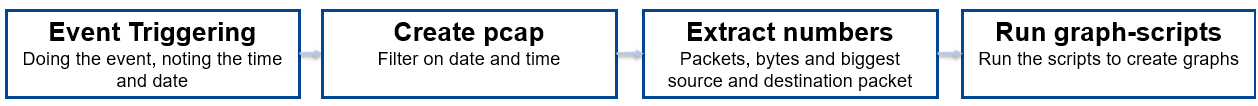
\includegraphics[width=\textwidth]{figures/GeneralProcedure.png}
    \caption{General Procedure}
    \label{fig:GeneralProcedure}
\end{figure}

To be able to run analysis on the data gathered from the different packet capturings (pcaps) and present it in an understandable way, two different programs were used; Wireshark and VsCode with pyshark. Wireshark were used to extract numbers from the pcaps and Visual Studio Code (VS Code) was used to generate graphs from the pcaps for the events. Even tough it is possible to use Wireshark to generate the same graphs as with VS Code, VS Code was selected because it is easier to generate graphs that have the same measures to compare and they are more ascetically pleasing to look at.
\\\\
When opening a pcap in Wireshark several statistics are possible to extract. By choosing the option of "Capture File Properties", total number of packets and bytes in the capture file are shown and were extracted. The numbers from each pcap were noted down and used as a value to compare both the events to each other and to the baseline. 
\\\\
In VS Code, python was used as the programming language as it includes the package pyshark which can be used towards tshark. Two scripts with a number of different if statements were used to generate the graphs depending on the users arguments passed to the script. The scripts only differs with if the user wants to display the graphs with number of packets or number of graphs on the y-axis. The code is displayed in its whole in appendix XXXX, and in pseudo code beneath in algorithm \ref{alg:GraphScript}. For each of the if statements, the same code block is included and are only shown once in algorithm \ref{alg:GraphScript}. The graphs are all generated with bytes and packets per 2 seconds, where the y-axis is defined in amount of packets or bytes and the x-axis defined as time. 

\begin{algorithm}
\caption{Script for generating graphs}\label{alg:GraphScript}
\begin{algorithmic}[1]
        \For{Each date of event} \Comment{Graph\_function start}
            \State Extract the packets from the right pcap
            \For{Each packet in pcap}
                \State Extract packet length in byte and time or add packet count to time
                \State Display graph
            \EndFor
        \EndFor \Comment{Graph\_function end}\\
    \If{Argument 2 is Outbound} \Comment{Set display filter to outbound traffic}
        \If{Argument 1 is Netatmo}
            \State Set display filter to "wlan.sa == Netatmo MAC address"
        \ElsIf{Argument 1 is Mill}
            \State Set display filter to "wlan.sa == Mill MAC address"
        \ElsIf{Argument 1 is Nedis}
            \State Set display filter to "wlan.sa == Nedis MAC address"    
        \EndIf\\
    \ElsIf{Argument 2 is Inbound} \Comment{Set display filter to inbound traffic}
        \If{Argument 1 is Netatmo}
            \State Set display filter to "wlan.da == Netatmo MAC address"
        \ElsIf{Argument 1 is Mill}
            \State Set display filter to "wlan.da == Mill MAC address"
        \ElsIf{Argument 1 is Nedis}
            \State Set display filter to "wlan.da == Nedis MAC address"  
        \EndIf\\
    \If{Argument 3 is Shower} \Comment{Event if-cases start}
        \State Set the dates from when the events occured 
        \State Graph\_function
    \ElsIf{Argument 3 is Cooking}
        \State Set the dates from when the events occured 
        \State Graph\_function
    \ElsIf{Argument 3 is Window}
        \State Set the dates from when the events occured 
        \State Graph\_function
    \ElsIf{Argument 3 is Weekend}
        \State Set the dates from when the events occured 
        \State Graph\_function
    \ElsIf{Argument 3 is Baseline}
        \State Set the dates from when the events occured 
        \State Graph\_function
    \EndIf \Comment{Event if-cases end}
\end{algorithmic}
\end{algorithm}

\begin{table}[H]
    \centering
    \caption{Overview of system arguments for scripts}
    \begin{adjustbox}{width=1\textwidth}
    \begin{tabular}{l|l|l|}
        \cline{2-3} & \textbf{Description} & \textbf{Values}\\ \hline
        \multicolumn{1}{|l|}{\textbf{Argument 1}} & Name of device & \begin{tabular}[c]{@{}l@{}}Netatmo\\ Mill\\ Nedis\end{tabular} \\ \hline
        \multicolumn{1}{|l|}{\textbf{Argument 2}} & Which packets to include & \begin{tabular}[c]{@{}l@{}}Inbound packets and bytes\\ Outbound packets and bytes\\ Inbound and outbound packets and bytes\end{tabular} \\ \hline
        \multicolumn{1}{|l|}{\textbf{Argument 3}} & Type of event & \begin{tabular}[c]{@{}l@{}}Cooking\\ Shower\\ Window\\ Weekend\\ Baseline\end{tabular} \\ \hline
        \multicolumn{1}{|l|}{\textbf{Argument 4}} & Maximum value for y-axis, in bytes or packets & "Numeric value" \\ \hline
    \end{tabular}
    \end{adjustbox}
    \label{tab:SystemArgumentsScripts}
\end{table}

To create a file for each of the events, a time filter were applied to the pcaps and then the remaining packets exported to a separate pcap that can be opened in Wireshark or make a graph out of to analyze each specific event. The time filter has the following format:

\begin{itemize}
\item \textbf{Format:} frame.time >= "Month Date, Year "Time"" && frame.time <= "Month Date, Year "Time""//
\item \textbf{Example:} frame.time >= "Jan 08, 2023 "19:30:00"" && frame.time <= "Jan 08, 2023 "20:40:00""
\end{itemize}

In this research, each event have been carried out 15 times, but to make the pages presentable and understandable to look at, only the first 12 graphs from the events are shown. The rest of the graphs follows the same pattern as the 10 first, but will be only be added in the appendix. The same applies to when comparing baseline traffic against the events. To be able to present this in an understandable way, only 7 of each category are chosen to be added to the graphical comparison. All calculations are added directly in this chapter as it is possible to do this in a presentable way without overloading the pages. For the weekend testing, all graphs are shown. 

\section{Baseline}
The capturing of baseline traffic were conducted over the course of 10 days in the same environment as the devices were when conducting the events. During the baseline, the devices have not been affected by the specific events, such as cooking, showering or window open in the same room as the devices resides. The baseline traffic will both be used to look at standard traffic from the devices and to compare this to the events in both graphs and calculations in sub chapter 5.3-5.5. The traffic from the capture file is encrypted on layer 2 (Wi-Fi) and therefore it is not possible to extract any values from the payload of the packets. This applies to all the devices.  
\subsection{Netatmo Baseline}
\textit{Figure \ref{fig:NetatmoBaselineTotalPackets}} and \textit{\ref{fig:NetatmoBaselineTotalBytes}} shows the graphs for Netatmo Home Coach from the baseline capturing from 6th of March 2023 to 15th of March 2023. 
\begin{figure} [H]
    \centering
    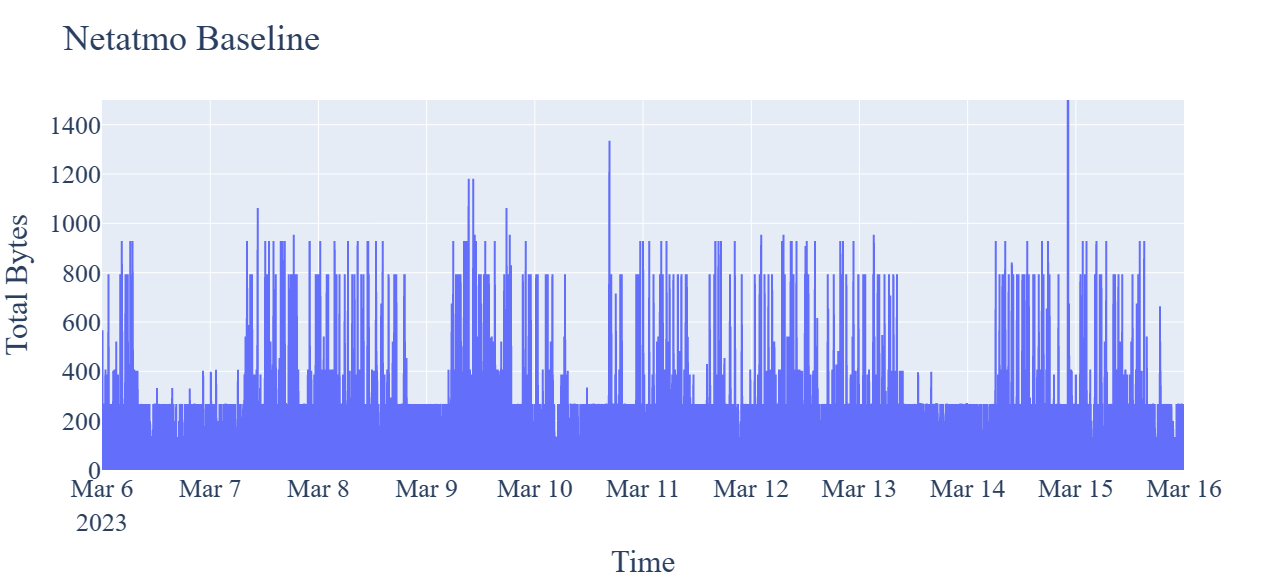
\includegraphics[scale=0.3]{figures/Netatmo_Baseline_TotalBytes.png}
    \caption{Netatmo Baseline Total Bytes}
    \label{fig:NetatmoBaselineTotalBytes}
\end{figure}

\begin{figure} [H]         
    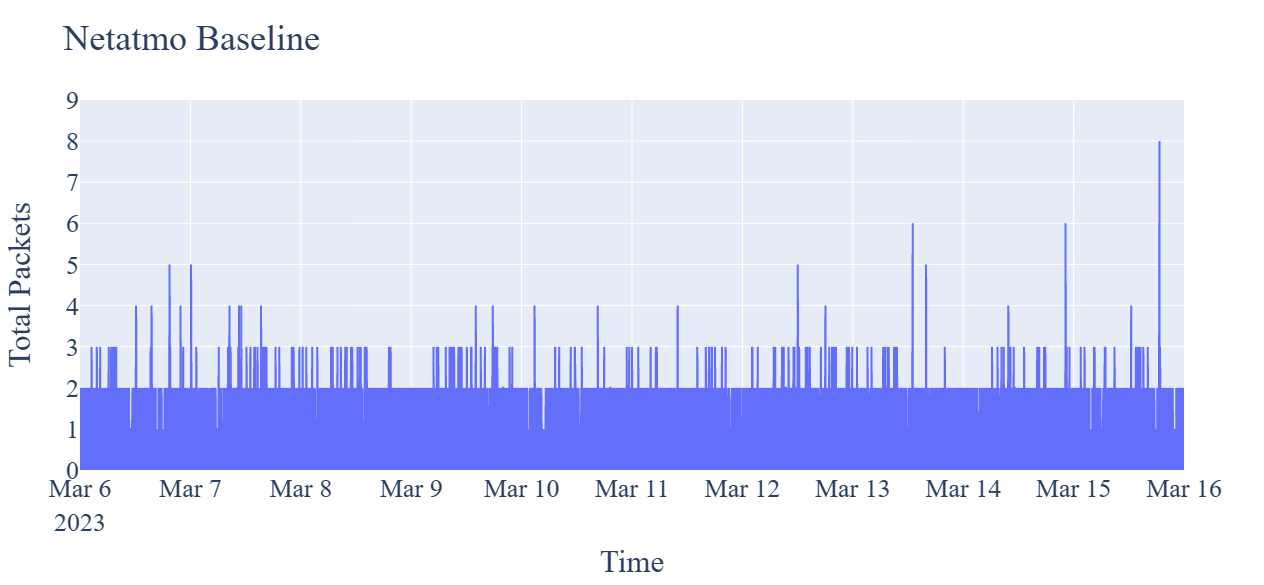
\includegraphics[scale=0.3]{figures/Netatmo_Baseline_TotalPackets.png}
    \caption{Netatmo Baseline Total Packets}
    \label{fig:NetatmoBaselineTotalPackets}
 \end{figure}

For the baseline graphs, it is possible to see that packets are sent continually at a rate of around 250 bytes per 2 seconds and 2 packets per 2 seconds. As these graphs shows the total packets and bytes sent and received, it can also be beneficial to look at what the graphs would look like if filtered on packets and bytes sent and packets and bytes received separately. 

\begin{figure}[H]
    \centering
    \begin{subfigure}[b]{0.7\textwidth}
        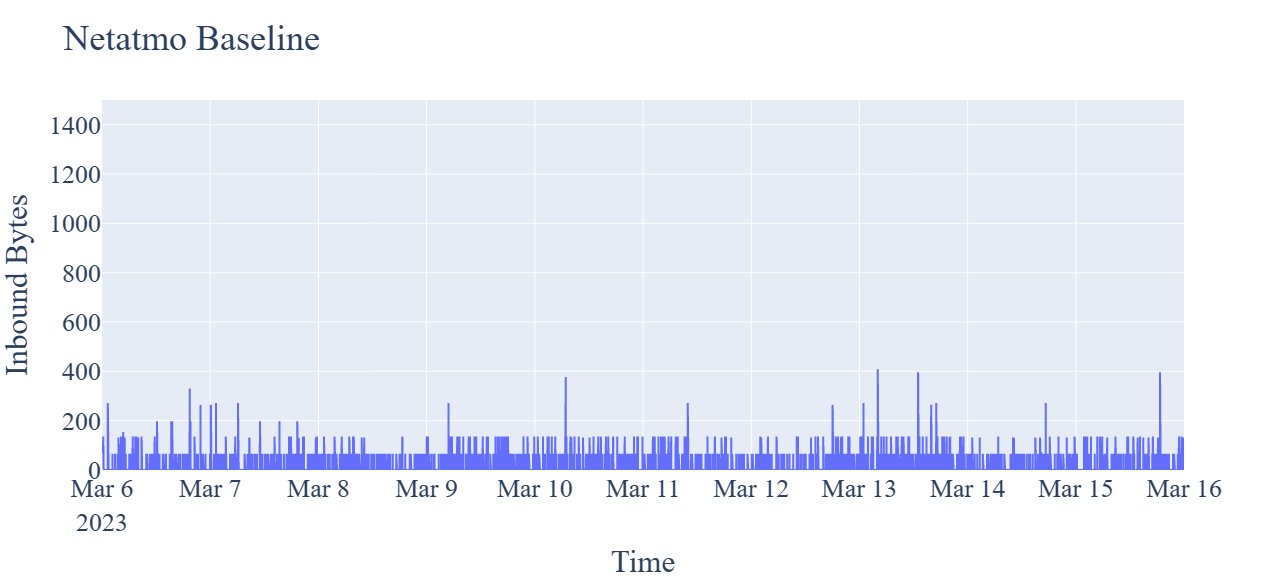
\includegraphics[width=\textwidth]{figures/Netatmo_Baseline_InboundBytes.png}
        \caption{Inbound Bytes}
        \label{fig:NetatmoBaselineInboundBytes}
    \end{subfigure}
    \begin{subfigure}[b]{0.7\textwidth}
        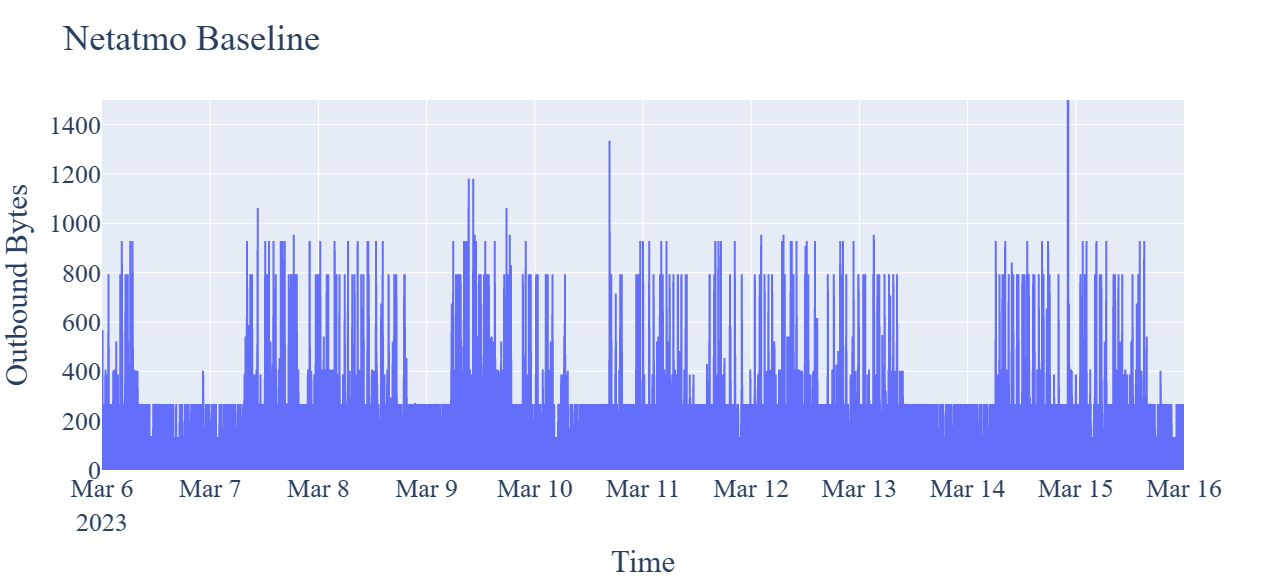
\includegraphics[width=\textwidth]{figures/Netatmo_Baseline_OutboundBytes.png}
        \caption{Outbound Bytes}
        \label{fig:NetatmoBaselineOutboundBytes}
    \end{subfigure}
    \caption{Netatmo Baseline Inbound and Outbound Bytes}
    \label{Fig:NetatmoBaselineOutandInboundBytes}
 \end{figure}

 \begin{figure}[H]
    \centering
    \begin{subfigure}[b]{0.7\textwidth}
        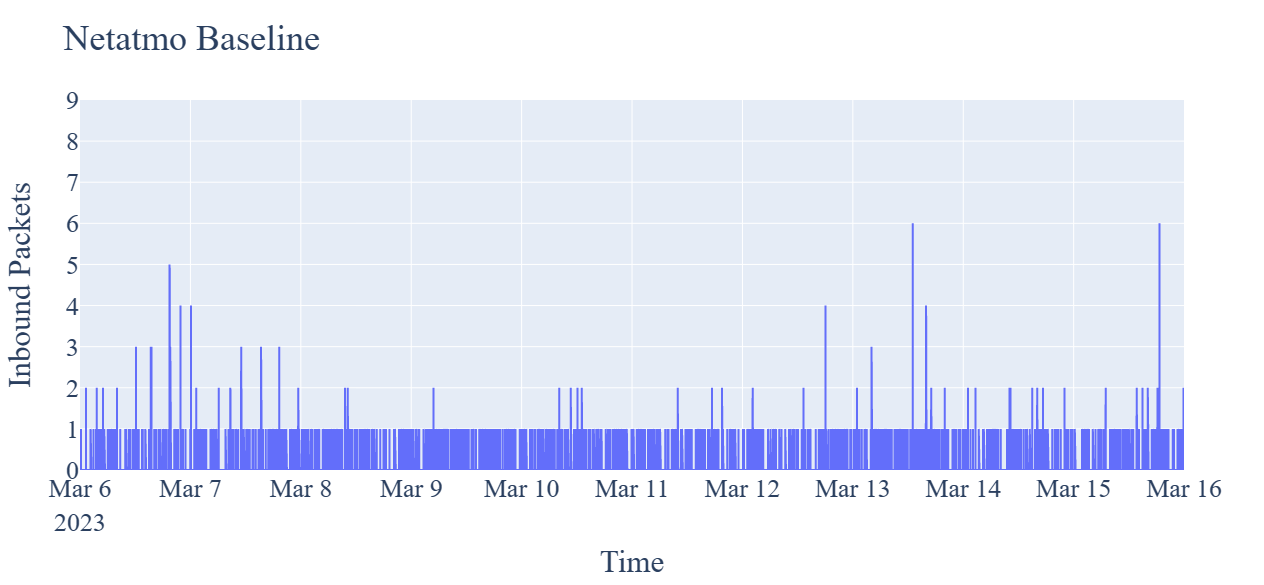
\includegraphics[width=\textwidth]{figures/Netatmo_Baseline_InboundPackets.png}
        \caption{Inbound Packets}
        \label{fig:NetatmoBaselineInboundPackets}
    \end{subfigure}
    \begin{subfigure}[b]{0.7\textwidth}
        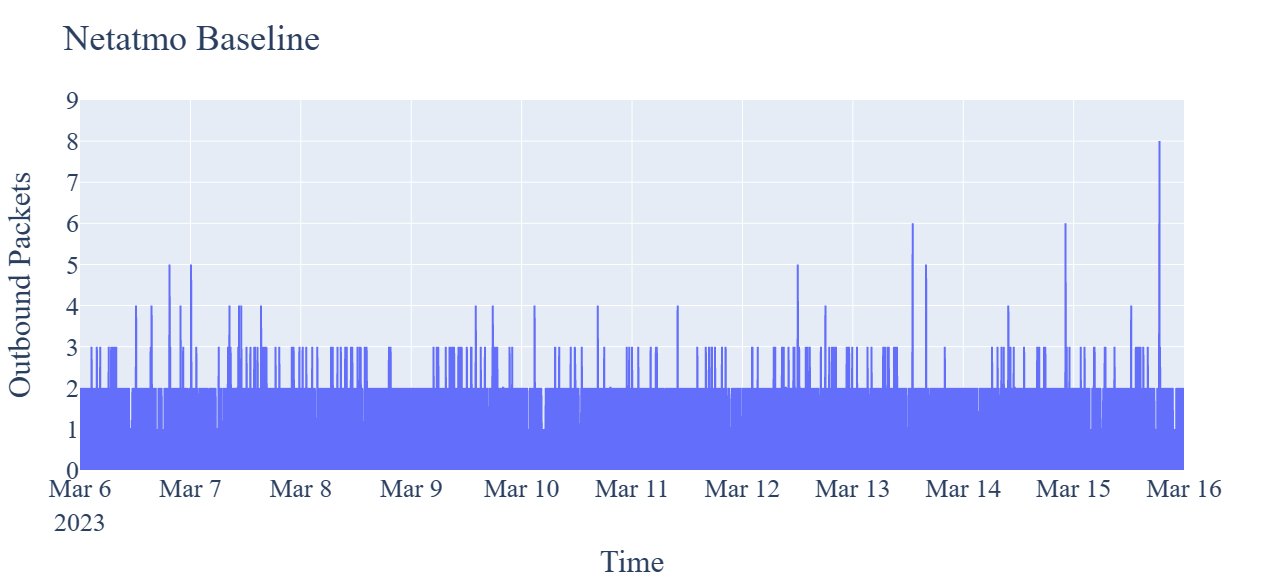
\includegraphics[width=\textwidth]{figures/Netatmo_Baseline_OutboundPackets.png}
        \caption{Outbound Packets}
        \label{fig:NetatmoBaselineOutboundPackets}
    \end{subfigure}
    \caption{Netatmo Baseline Inbound and Outbound Packets}
    \label{Fig:NetatmoBaselineOutandInboundPackets}
 \end{figure}
For the inbound and outbound bytes for Netatmo, \textit{Figure \ref{Fig:NetatmoBaselineOutandInboundBytes}}, it is clear to see that the device sends a lot more bytes than it receives. The same pattern appears in \textit{Figure \ref{Fig:NetatmoBaselineOutandInboundPackets}} for packets. Calculations made on the baseline traffic are presented in Table \ref{tab:NetatmoBaselineCalculations}. 
\begin{table}[H]
    \caption{Calculations for Netatmo Baseline Capture}
    \centering
    \begin{tabular}{ll|l|}
        \cline{3-3}                                               &                               &             \textbf{Numbers} \\ \hline
        \multicolumn{1}{|c|}{\multirow{4}{*}{\textbf{Total}}}    & Packets              & 110,735         \\ \cline{2-3} 
        \multicolumn{1}{|c|}{}                                   & Bytes                & 14,959,396       \\ \cline{2-3} 
        \multicolumn{1}{|c|}{}                                   & Average bytes/second & 17               \\ \cline{2-3} 
        \multicolumn{1}{|c|}{}                                   & Average packet size  & 135 bytes        \\ \hline
        \multicolumn{1}{|l|}{\multirow{5}{*}{\textbf{Inbound}}}  & Packets              & 1,042            \\ \cline{2-3} 
        \multicolumn{1}{|l|}{}                                   & Bytes                & 83,446           \\ \cline{2-3} 
        \multicolumn{1}{|l|}{}                                   & Average bytes/second & 0                \\ \cline{2-3} 
        \multicolumn{1}{|l|}{}                                   & Average packet size  & 80 bytes          \\ \cline{2-3} 
        \multicolumn{1}{|l|}{}                                   & Biggest packet       & 377 bytes        \\ \hline
        \multicolumn{1}{|l|}{\multirow{5}{*}{\textbf{Outbound}}} & Packets              & 109,693          \\ \cline{2-3} 
        \multicolumn{1}{|l|}{}                                   & Bytes                & 14,875,950       \\ \cline{2-3} 
        \multicolumn{1}{|l|}{}                                   & Average bytes/second & 17               \\ \cline{2-3} 
        \multicolumn{1}{|l|}{}                                   & Average packet size  & 136 bytes         \\ \cline{2-3} 
        \multicolumn{1}{|l|}{}                                   & Biggest packet       & 1,150 bytes       \\ \hline
    \end{tabular}
    \label{tab:NetatmoBaselineCalculations}
\end{table}
Comparing the inbound(Figure \ref{fig:NetatmoBaselineInboundBytes} and \ref{fig:NetatmoBaselineInboundPackets}) and outbound(Figure \ref{fig:NetatmoBaselineOutboundBytes} and \ref{fig:NetatmoBaselineOutboundPackets}) graphs with the total graphs (Figure \ref{fig:NetatmoBaselineTotalBytes} and Figures \ref{fig:NetatmoBaselineTotalPackets}), shows that the outbound graphs stands for a majority of the packets and they are very similar to the total graphs. The same is numerically shown in Table \ref{tab:NetatmoBaselineCalculations}, where over 99\% of the total packets are outbound traffic. The majority of packets sent from Netatmo are packets labeled "Data" with a size of 134 bytes, which makes up 98,3\% of the packets from the capture file. Therefore, it will be better to only display the events with graphs for total traffic to evaluate and analyze further on. 

\subsection{Mill Baseline}
\textit{Figure \ref{fig:MillBaselineTotalPackets}} and \textit{\ref{fig:MillBaselineTotalBytes}} shows the graphs for Mill from the baseline capturing from 6th of March 2023 to 15th of March 2023. 
\begin{figure} [H]
    \centering
    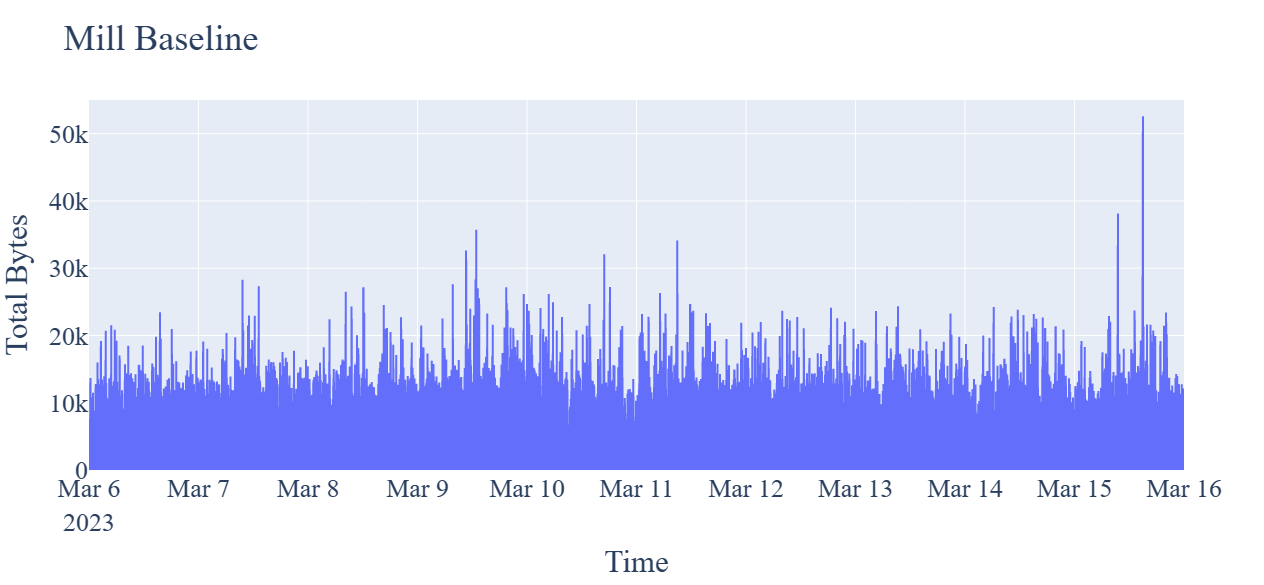
\includegraphics[scale=0.3]{figures/Mill_Baseline_TotalBytes.png}
    \caption{Mill Baseline Total Bytes}
    \label{fig:MillBaselineTotalBytes}
\end{figure}

\begin{figure} [H]
    \centering
    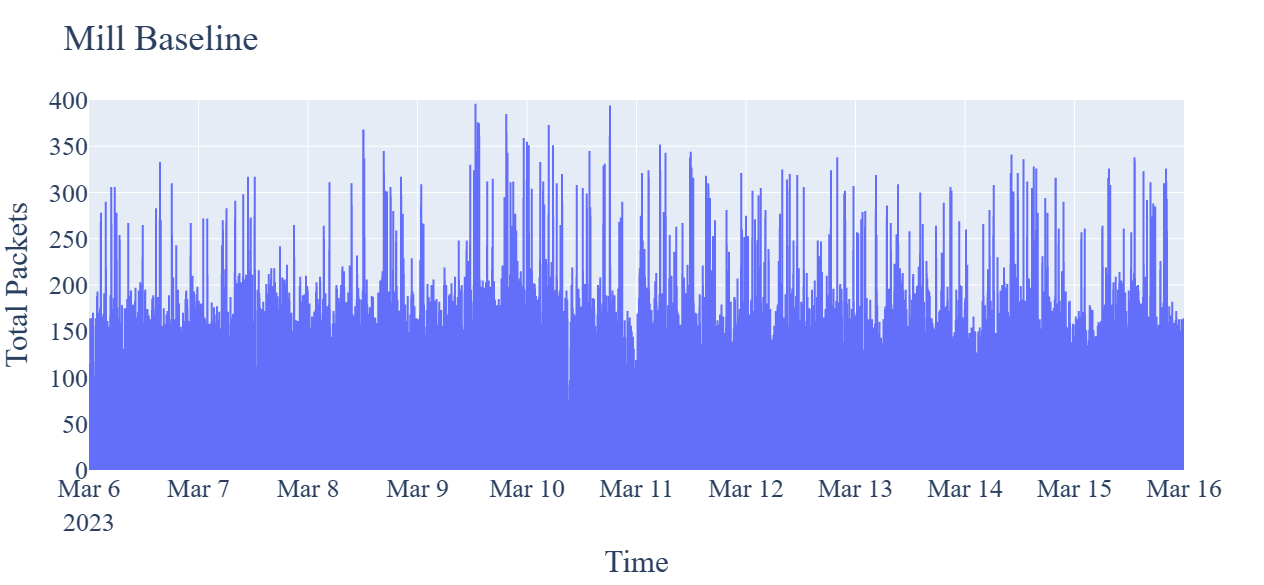
\includegraphics[scale=0.3]{figures/Mill_Baseline_TotalPackets.png}
    \caption{Mill Baseline Total Packets}
    \label{fig:MillBaselineTotalPackets}
 \end{figure}

The baseline traffic for Mill shows that the traffic varies a lot. As this device does not send live updates, but every minute, more spikes are included as it does not always send packets. It is also possible to see the spikes more clearly if the time range is smaller, this will be visible further when looking at the baseline comparison graphs for each event. 

Graphs for inbound and outbound traffic have also been made for Mill, to see the differences for the packets sent. Figure \ref{Fig:MillBaselineOutandInboundBytes} and \ref{Fig:MillBaselineOutandInboundPackets} displays the different graphs for each of the traffic directions. Numerical calculations for the baseline traffic are presented in Table \ref{tab:MillBaselineCalculations}. 

\begin{figure}[H]
    \centering
    \begin{subfigure}[b]{0.7\textwidth}
        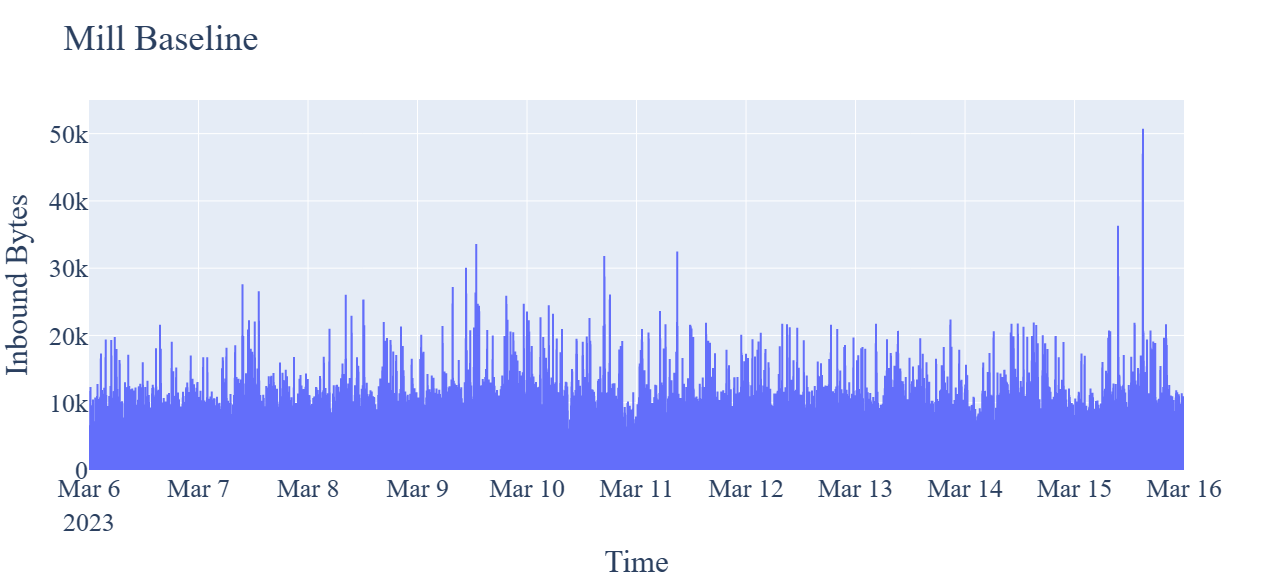
\includegraphics[width=\textwidth]{figures/Mill_Baseline_InboundBytes.png}
        \caption{Inbound Bytes}
        \label{fig:MillBaselineInboundBytes}
    \end{subfigure}
    \begin{subfigure}[b]{0.7\textwidth}
        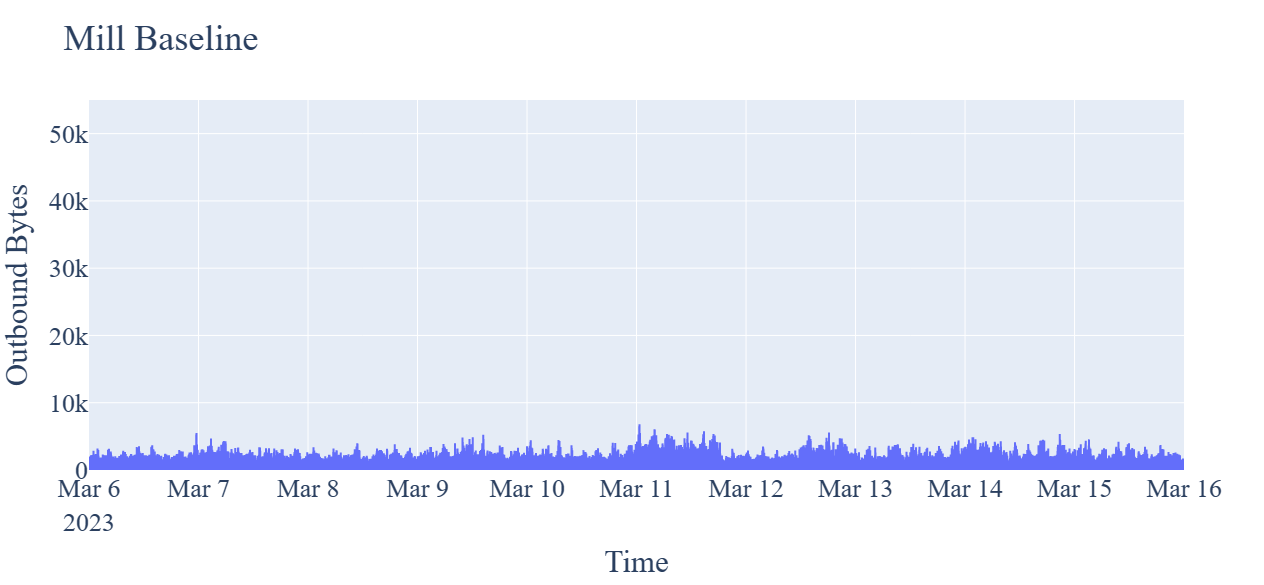
\includegraphics[width=\textwidth]{figures/Mill_Baseline_OutboundBytes.png}
        \caption{Outbound Bytes}
        \label{fig:MillBaselineOutboundBytes}
    \end{subfigure}
    \caption{Mill Baseline Inbound and Outbound Bytes}
    \label{Fig:MillBaselineOutandInboundBytes}
 \end{figure}

 \begin{figure}[H]
    \centering
    \begin{subfigure}[b]{0.7\textwidth}
        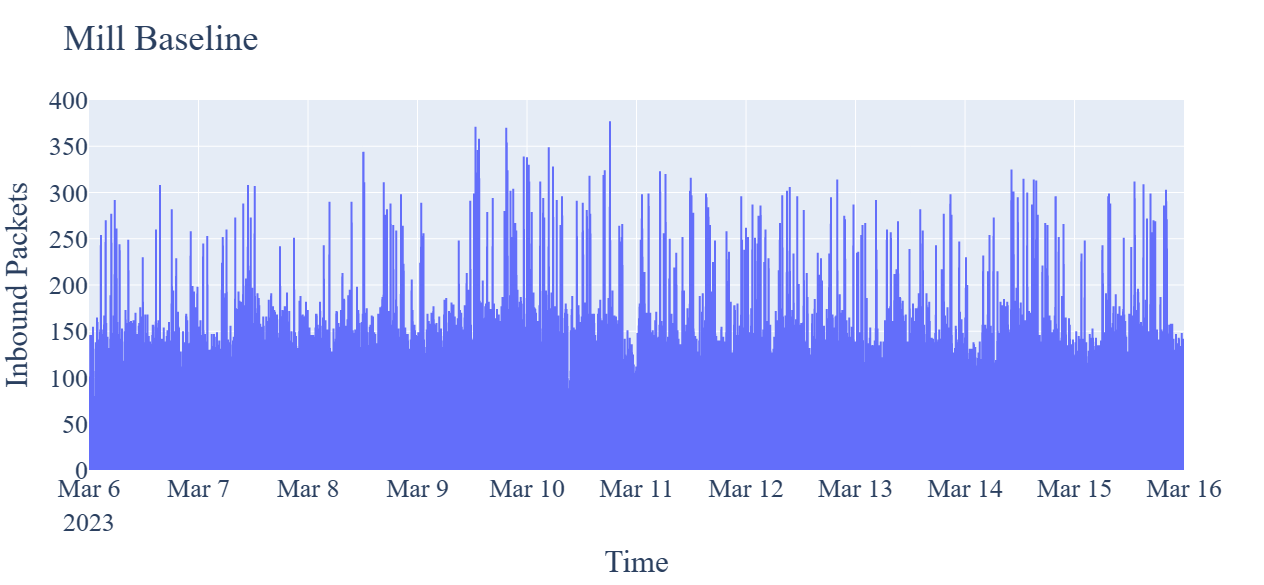
\includegraphics[width=\textwidth]{figures/Mill_Baseline_InboundPackets.png}
        \caption{Inbound Packets}
        \label{fig:MillBaselineInboundPackets}
    \end{subfigure}
    \begin{subfigure}[b]{0.7\textwidth}
        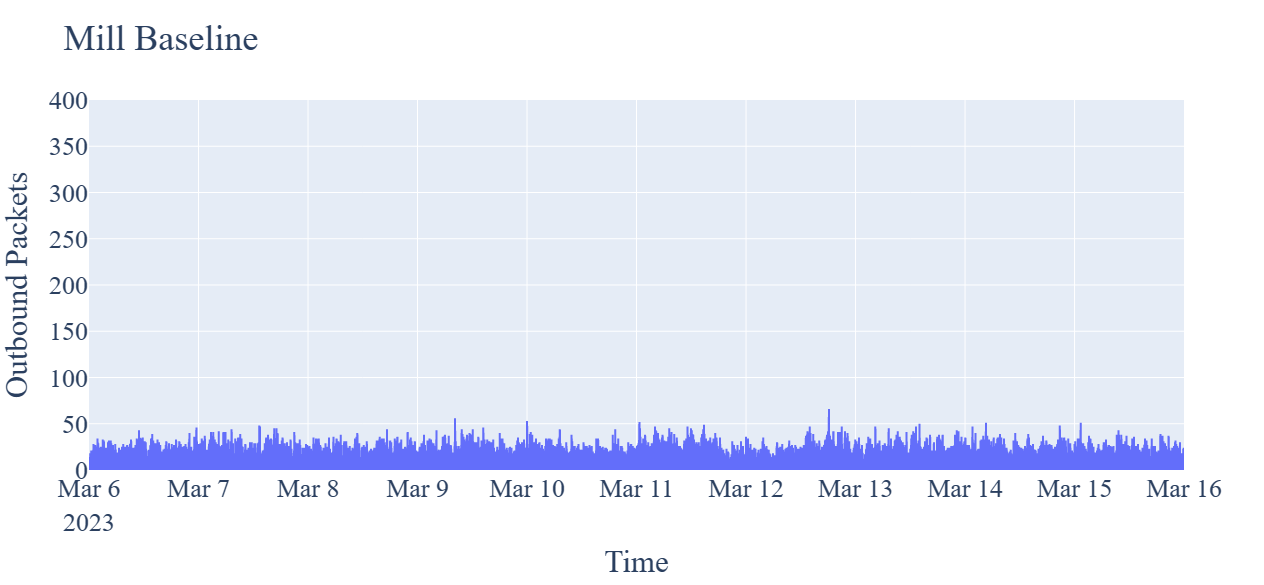
\includegraphics[width=\textwidth]{figures/Mill_Baseline_OutboundPackets.png}
        \caption{Outbound Packets}
        \label{fig:MillBaselineOutboundPackets}
    \end{subfigure}
    \caption{Mill Baseline Inbound and Outbound Packets}
    \label{Fig:MillBaselineOutandInboundPackets}
 \end{figure}

\begin{table}[H]
    \caption{Calculations for Mill Baseline Capture}
    \centering
    \begin{tabular}{ll|l|}
        \cline{3-3}                                              &                      & \textbf{Numbers} \\ \hline
        \multicolumn{1}{|c|}{\multirow{4}{*}{\textbf{Total}}}    & Packets              & 1,236,753       \\ \cline{2-3} 
        \multicolumn{1}{|c|}{}                                   & Bytes                & 129,253,290     \\ \cline{2-3} 
        \multicolumn{1}{|c|}{}                                   & Average bytes/second & 149             \\ \cline{2-3} 
        \multicolumn{1}{|c|}{}                                   & Average packet size  & 105 bytes       \\ \hline
        \multicolumn{1}{|l|}{\multirow{5}{*}{\textbf{Inbound}}}  & Packets              & 942,112         \\ \cline{2-3} 
        \multicolumn{1}{|l|}{}                                   & Bytes                & 95,458,773      \\ \cline{2-3} 
        \multicolumn{1}{|l|}{}                                   & Average bytes/second & 110             \\ \cline{2-3} 
        \multicolumn{1}{|l|}{}                                   & Average packet size  & 101 bytes       \\ \cline{2-3} 
        \multicolumn{1}{|l|}{}                                   & Biggest packet       & 1593 bytes      \\ \hline
        \multicolumn{1}{|l|}{\multirow{5}{*}{\textbf{Outbound}}} & Packets              & 294,640         \\ \cline{2-3} 
        \multicolumn{1}{|l|}{}                                   & Bytes                & 33,794,517      \\ \cline{2-3} 
        \multicolumn{1}{|l|}{}                                   & Average bytes/second & 39              \\ \cline{2-3} 
        \multicolumn{1}{|l|}{}                                   & Average packet size  & 115 bytes       \\ \cline{2-3} 
        \multicolumn{1}{|l|}{}                                   & Biggest packet       & 456 bytes       \\ \hline
    \end{tabular}
    \label{tab:MillBaselineCalculations}
\end{table}

As Figure \ref{Fig:MillBaselineOutandInboundBytes} and \ref{Fig:MillBaselineOutandInboundPackets} shows, the device receives a lot more packets and bytes than it sends off. And as the inbound graphs do not differ much from the total graphs, it will be best to proceed with the analysis in a total traffic aspect where both inbound and outbound traffic are included. This is also reflected in Table \ref{tab:MillBaselineCalculations}, which shows that 76\% of packets and 74\% of bytes are received.

\subsection{Nedis Baseline}
\textit{Figure \ref{fig:NedisBaselineTotalPackets}} and \textit{\ref{fig:NedisBaselineTotalBytes}} shows the graphs for Nedis from the baseline capturing from 6th of March 2023 to 15th of March 2023. 
\begin{figure} [H]
    \centering
    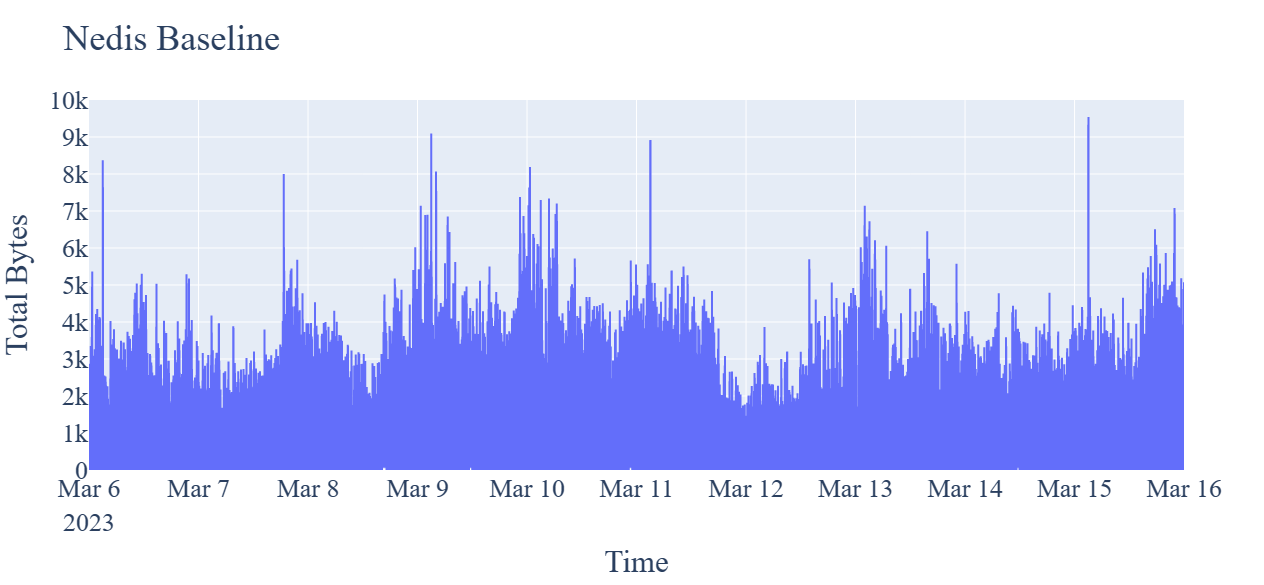
\includegraphics[scale=0.3]{figures/Nedis_Baseline_TotalBytes.png}
    \caption{Nedis Baseline Total Bytes}
    \label{fig:NedisBaselineTotalBytes}
\end{figure}

\begin{figure} [H]         
    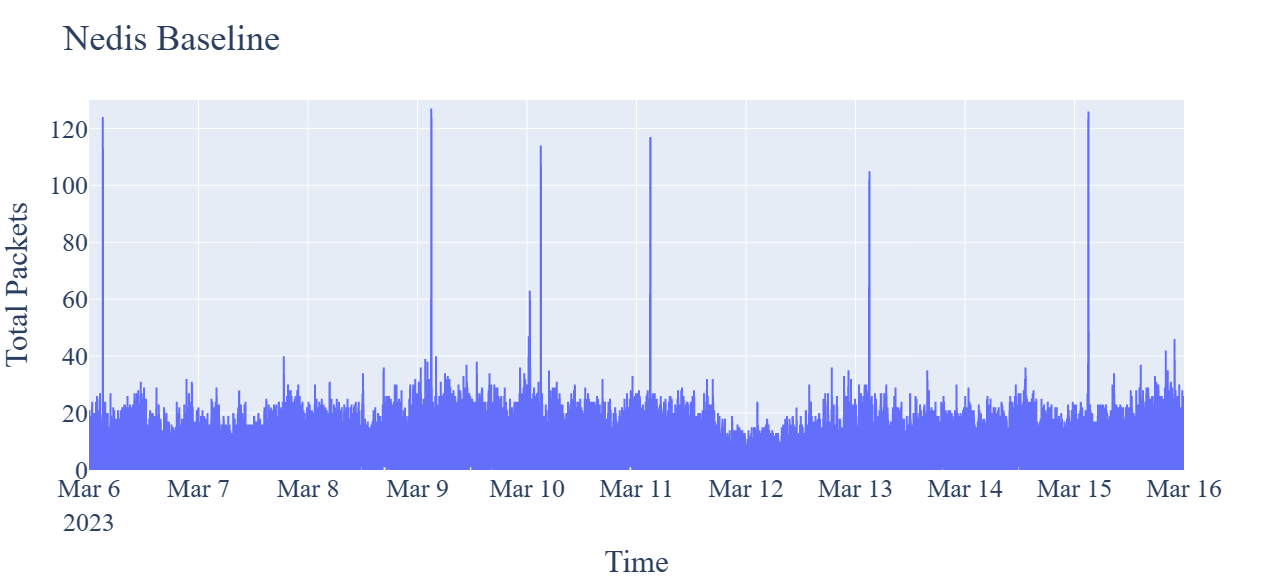
\includegraphics[scale=0.3]{figures/Nedis_Baseline_TotalPackets.png}
    \caption{Nedis Baseline Total Packets}
    \label{fig:NedisBaselineTotalPackets}
 \end{figure}

The traffic sent and received by Nedis is characterized by several spikes even though the traffic varies some. The larger spikes, which are more visible in Figure \ref{fig:NedisBaselineTotalPackets}, showing the packets, occurs almost everyday. Since traffic is encrypted, it is not possible to see what these spikes are, but for further analysis it is important to understand that normal traffic for the device, can be large spikes occurring around the same time each night the spike occurs. Even though this thesis will not go further into looking at what the spikes actually are, it can be interesting to see if they are inbound or outbound traffic. 

To look at the differences in inbound and outbound traffic for Nedis, Figure \ref{Fig:NedisBaselineOutandInboundBytes} and \ref{Fig:NedisBaselineOutandInboundPackets} are displayed. Figure \ref{fig:NedisBaselineOutboundPackets} shows that the spikes are packets which the device receives.
Even though the graphs for inbound and outbound traffic from Nedis looks more similar, the calculations presented in Table \ref{tab:NedisBaselineCalculations}, shows that 81\% of the packets and 70\% of the bytes in the baseline are traffic sent from the device. Looking at the graphs in total will therefore give the most to analyze. Another aspect of looking at the graphs in total, compared to inbound and outbound separately is that since the traffic is encrypted on the layer 2, it is not possible to know what makes the possible changes. 

\begin{figure}[H]
    \centering
    \begin{subfigure}[b]{0.7\textwidth}
        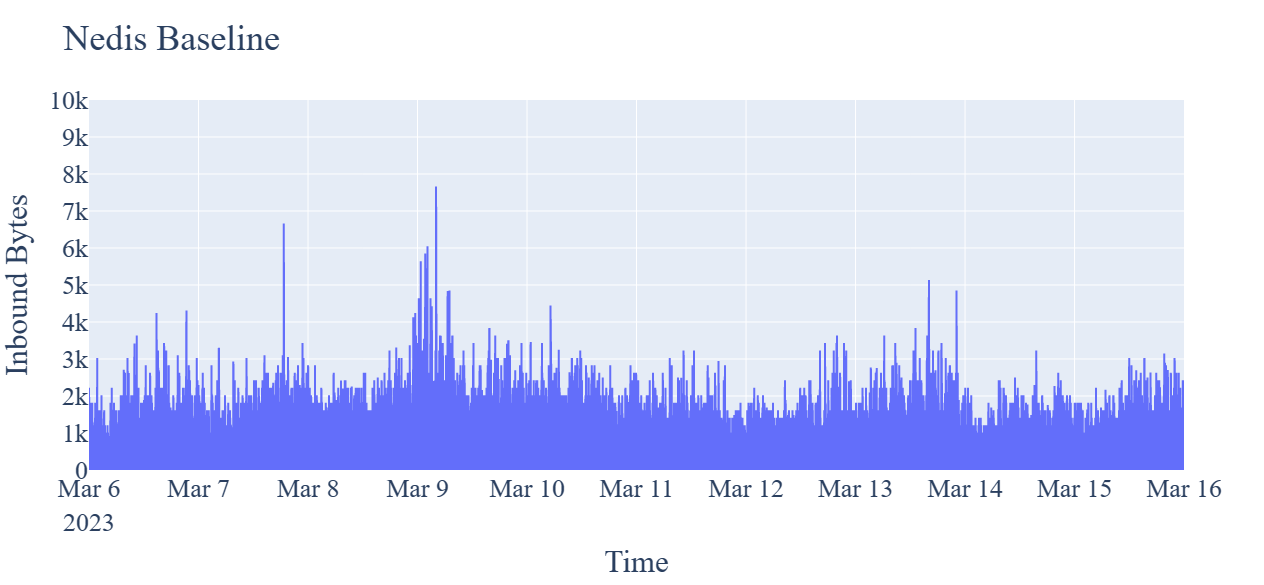
\includegraphics[width=\textwidth]{figures/Nedis_Baseline_InboundBytes.png}
        \caption{Inbound Bytes}
        \label{fig:NedisBaselineInboundBytes}
    \end{subfigure}
    \begin{subfigure}[b]{0.7\textwidth}
        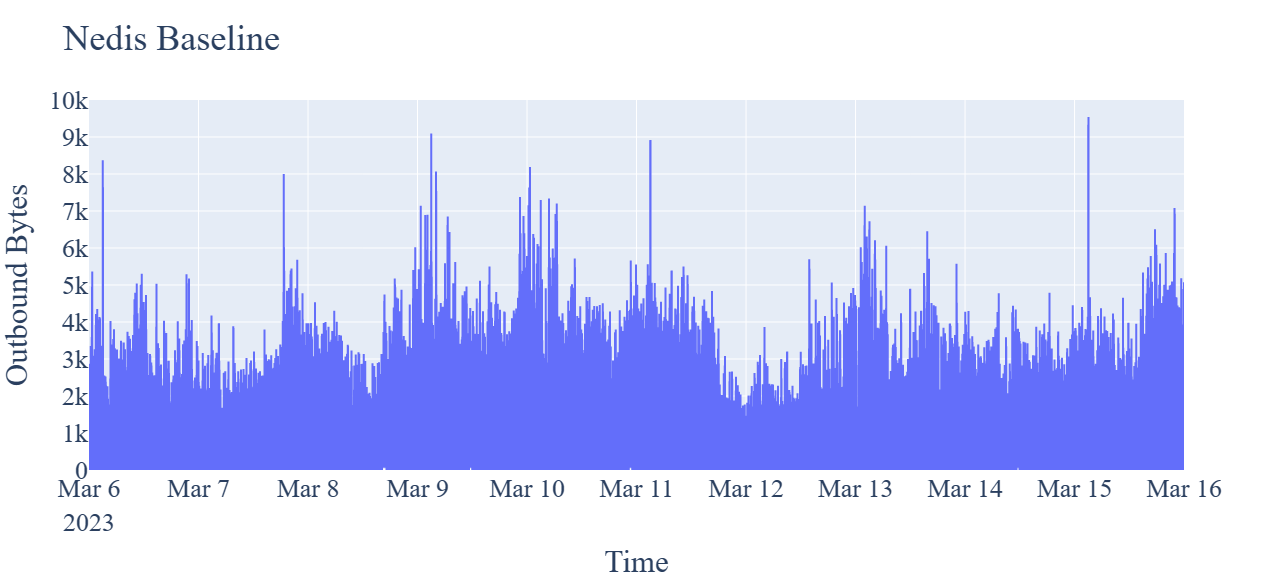
\includegraphics[width=\textwidth]{figures/Nedis_Baseline_OutboundBytes.png}
        \caption{Outbound Bytes}
        \label{fig:NedisBaselineOutboundBytes}
    \end{subfigure}
    \caption{Nedis Baseline Inbound and Outbound Bytes}
    \label{Fig:NedisBaselineOutandInboundBytes}
 \end{figure}

 \begin{figure}[H]
    \centering
    \begin{subfigure}[b]{0.7\textwidth}
        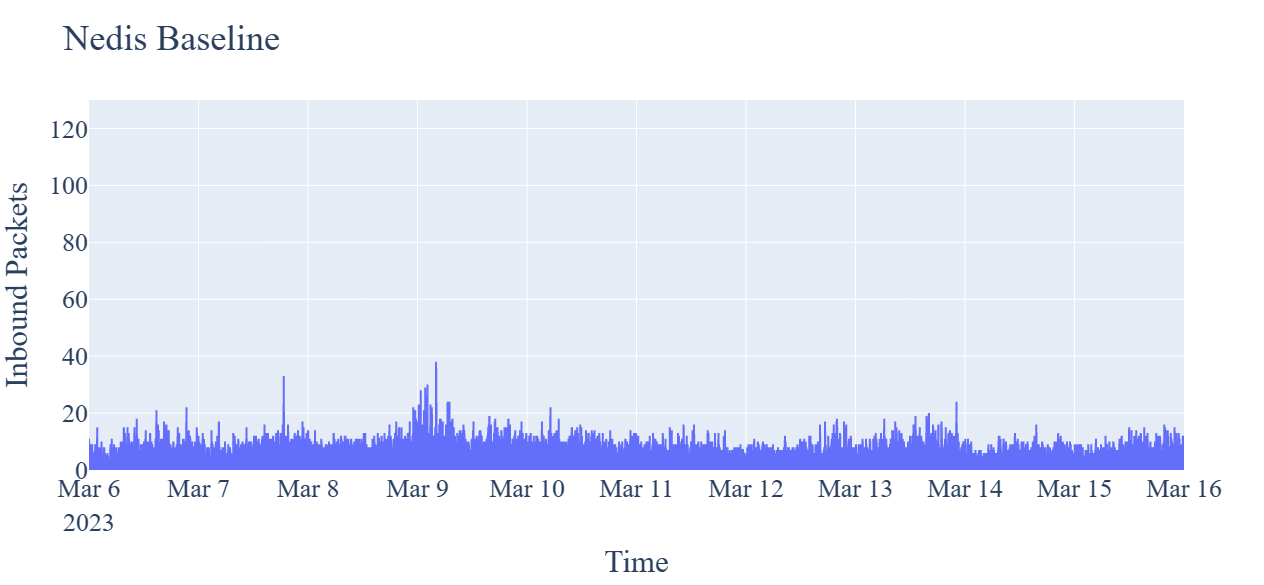
\includegraphics[width=\textwidth]{figures/Nedis_Baseline_InboundPackets.png}
        \caption{Inbound Packets}
        \label{fig:NedisBaselineInboundPackets}
    \end{subfigure}
    \begin{subfigure}[b]{0.7\textwidth}
        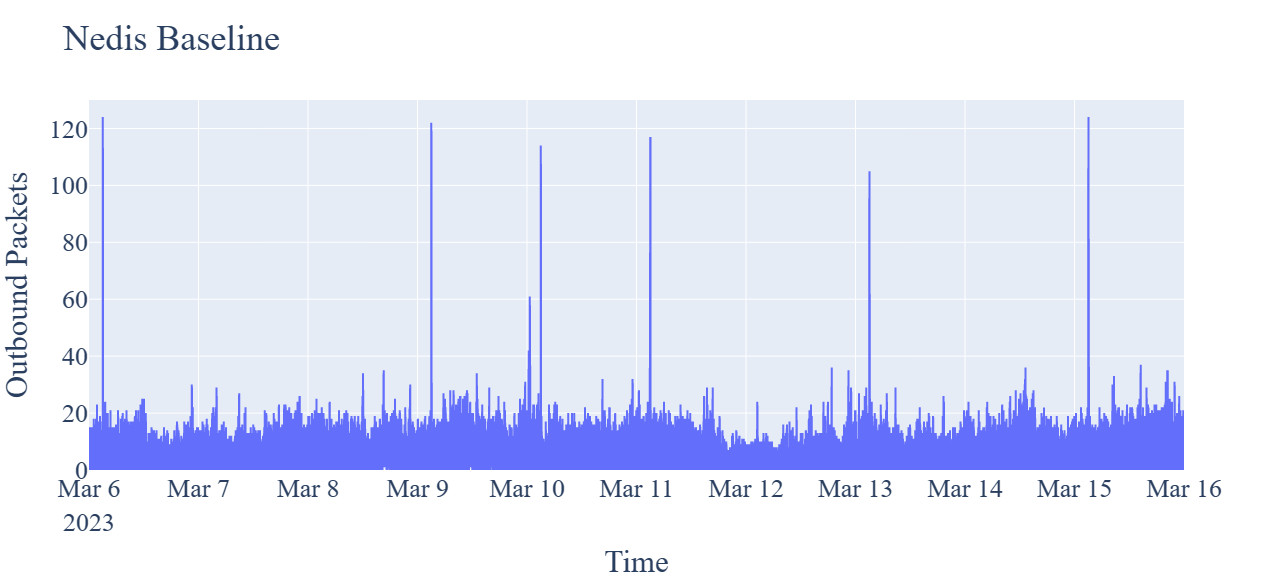
\includegraphics[width=\textwidth]{figures/Nedis_Baseline_OutboundPackets.png}
        \caption{Outbound Packets}
        \label{fig:NedisBaselineOutboundPackets}
    \end{subfigure}
    \caption{Nedis Baseline Inbound and Outbound Packets}
    \label{Fig:NedisBaselineOutandInboundPackets}
 \end{figure}
 
\begin{table}[H]
    \caption{Calculations for Nedis Baseline Capture}
    \centering
    \begin{tabular}{ll|l|}
        \cline{3-3}                                               &                               &             \textbf{Numbers} \\ \hline
        \multicolumn{1}{|c|}{\multirow{4}{*}{\textbf{Total}}}    & Packets              & 2,428,701         \\ \cline{2-3} 
        \multicolumn{1}{|c|}{}                                   & Bytes                & 295,022,494       \\ \cline{2-3} 
        \multicolumn{1}{|c|}{}                                   & Average bytes/second & 341               \\ \cline{2-3} 
        \multicolumn{1}{|c|}{}                                   & Average packet size  & 121 bytes        \\ \hline
        \multicolumn{1}{|l|}{\multirow{5}{*}{\textbf{Inbound}}}  & Packets              & 451,495           \\ \cline{2-3} 
        \multicolumn{1}{|l|}{}                                   & Bytes                & 88,595,049        \\ \cline{2-3} 
        \multicolumn{1}{|l|}{}                                   & Average bytes/second & 102                \\ \cline{2-3} 
        \multicolumn{1}{|l|}{}                                   & Average packet size  & 196 bytes         \\ \cline{2-3} 
        \multicolumn{1}{|l|}{}                                   & Biggest packet       & 522 bytes        \\ \hline
        \multicolumn{1}{|l|}{\multirow{5}{*}{\textbf{Outbound}}} & Packets              & 1,977,206         \\ \cline{2-3} 
        \multicolumn{1}{|l|}{}                                   & Bytes                & 206,427,445      \\ \cline{2-3} 
        \multicolumn{1}{|l|}{}                                   & Average bytes/second & 238               \\ \cline{2-3} 
        \multicolumn{1}{|l|}{}                                   & Average packet size  & 104 bytes         \\ \cline{2-3} 
        \multicolumn{1}{|l|}{}                                   & Biggest packet       & 485 bytes       \\ \hline
    \end{tabular}
    \label{tab:NedisBaselineCalculations}
\end{table} 


\section{Test Case 1: Cooking}
This chapter presents the results and analysis conducted on Test Case 1: Cooking. The first subsection will present general information applicable to all the devices, and the following subsections will present the result and analysis for each of the devices separately. 
\subsection{General}
The cooking events are 10 in total and are presented in Table \ref{tab:CookingDates}. Every device has the same dates for this event. 
\begin{table}[!hbtp]
    \centering
    \caption{Date and time for Test Case 1: Cooking Events}
    \begin{adjustbox}{width=1\textwidth}
            \begin{tabular}{l|l|l|l|l|l|l|l|l|l|l|}
            \cline{2-11} & 08.01 & 09.01 & 11.01 & 16.01 & 18.01 & 19.01 & 25.01 & 30.01 & 31.01 & 01.02 \\
            \hline
            \multicolumn{1}{|l|}{Started event}  & 15:58 & 15:59 & 16:05 & 16:02 & 16:04 & 16:01 & 16:02 & 16:01 & 16:01 & 16:02 \\ 
            \hline
            \multicolumn{1}{|l|}{Finished event} & 16:22 & 16:21 & 16:37 & 16:25 & 16:25 & 16:18 & 16:13 & 16:19 & 16:21 & 16:22 \\ \hline
            \end{tabular}
    \end{adjustbox}
    \label{tab:CookingDates}
\end{table}
\FloatBarrier

To be able to look even further into differences from when the devices are in an environment when an event is ongoing and when it is in the same environment, but without any event ongoing, graphs and calculations from the baseline traffic are used to compare. To choose a time for the baseline traffic, the values in Table \ref{tab:CookingDates} are used. To have the same amount of time on each event the earliest start time and the latest finish time are used as filtering values for each of the pcaps from capturing the cooking event. The values were then added 30 minutes before and after and used as a the start and finish time for the events, while the actual event time given by Table \ref{tab:CookingDates} are marked red on the graphs. This gives the following values to use for further analysis:

\begin{itemize}
    \item Earliest Event Start: 15:58
    \item Latest Event Finished: 16:37
    \item Packet Capture Files Start: 15:28
    \item Packet Capture Files End: 17:07
\end{itemize}

This gives the following filters added to create the pcaps for each event:

\begin{itemize}
    \item frame.time >= "Month Date, Year 15:28:00" && frame.time <= "Month Date, Year 17:07:00"
\end{itemize}

\newpage
\subsection{Netatmo}
Table \ref{tab:NetatmoCookingCalculations} presents calculations from all these events and Table \ref{tab:NetatmoBaselineCookingCalculations} presents the calculations from all the corresponding baseline pcaps. Table \ref{tab:NetatmoComparingBaselineAndCookingCalculations} compares the average and standard deviation (std deviation) values from the events to the baseline. Figure \ref{fig:NetatmoCookingCalculations} presents a graphical overview of the packets and bytes from Table \ref{tab:NetatmoCookingCalculations} including average values. The graphs in Figure \ref{fig:NetatmoCookingBytes1}, \ref{fig:NetatmoCookingBytes2}, \ref{fig:NetatmoCookingPackets1} and \ref{fig:NetatmoCookingPackets2} shows both bytes and packets for the cooking events in comparison with the baseline captures. The actual events are placed on the left side of the figure and are framed in red, the baseline graphs are placed on the right side of the figure and are marked in blue. The area marked red on the event graphs are when the event was ongoing, and not included in the baseline graphs as no event was ongoing and is only used for comparison. 

\begin{table}[H]
    \centering
    \caption{Netatmo Cooking Calculations}
    \begin{tabular}{|l|l|l|l|l|l|}
    \hline
        \textbf{Event dates} & \textbf{Packets} & \textbf{Bytes} & \textbf{Biggest packet} \\ \hline
        08.jan & 901 & 123,630 & 407 bytes\\ \hline
        09.jan & 703 & 97,019 & 407 bytes \\ \hline
        11.jan & 847 & 114,473 & 407 bytes\\ \hline
        16.jan & 1,082 & 146,001 & 407 bytes\\ \hline
        18.jan & 948 & 129,907 & 407 bytes\\ \hline
        19.jan & 828 & 111,629 & 407 bytes \\ \hline
        25.jan & 430 & 58,926 & 407 bytes \\ \hline
        30.jan & 815 & 110,838 & 407 bytes \\ \hline
        31.jan & 864 & 115,302 & 136 bytes \\ \hline
        01.feb & 805 & 109,050 & 407 bytes \\ \hline
    \end{tabular}
    \label{tab:NetatmoCookingCalculations}
\end{table}

\begin{table}[!ht]
    \centering
    \caption{Netatmo Baseline Cooking Calculations}
    \begin{tabular}{|l|l|l|l|}
    \hline
        \textbf{Baseline} & \textbf{Packets} & \textbf{Bytes} & \textbf{Biggest packet} \\ \hline
        06.mar & 584 & 77,780 & 134 bytes\\ \hline
        07.mar & 972 & 132,406 & 407 bytes\\ \hline
        08.mar & 697 & 94,730 & 407 bytes \\ \hline
        09.mar & 868 & 117,020 & 407 bytes \\ \hline
        10.mar & 825 & 111,863 & 407 bytes \\ \hline
        11.mar & 745 & 101,534 & 407 bytes \\ \hline
        12.mar & 626 & 84,987 & 407 bytes \\ \hline
        13.mar & 764 & 101,772 & 136 bytes \\ \hline
        14.mar & 750 & 102,396 & 407 bytes \\ \hline
        15.mar & 812 & 108,703 & 407 bytes \\ \hline
    \end{tabular}
    \label{tab:NetatmoBaselineCookingCalculations}
\end{table}

\begin{table}[H]
    \centering
    \caption{Comparing Cooking and Baseline Calculations for Netatmo}
    \begin{tabular}{c|l|l|l|l|}
        \cline{2-5}
        \multicolumn{1}{l|}{}                                              & \textbf{Type} & \textbf{Packets} & \textbf{Bytes} & \textbf{Biggest packet} \\ \hline
        \multicolumn{1}{|c|}{\multirow{2}{*}{\textbf{Average}}}            & Event         & 822              & 111,678        & 380 bytes               \\ \cline{2-5} 
        \multicolumn{1}{|c|}{}                                             & Baseline      & 764              & 103,319        & 353 bytes                \\ \hline
        \multicolumn{1}{|c|}{\multirow{2}{*}{\textbf{Standard deviation}}} & Event         & 170              & 22,802         & 86 bytes                 \\ \cline{2-5} 
        \multicolumn{1}{|c|}{}                                             & Baseline      & 114              & 15,650         & 115 bytes               \\ \hline          
    \end{tabular}
    \label{tab:NetatmoComparingBaselineAndCookingCalculations}
\end{table}

\begin{figure}[H]
    \centering
    \begin{subfigure}{1\textwidth}
       \centering
       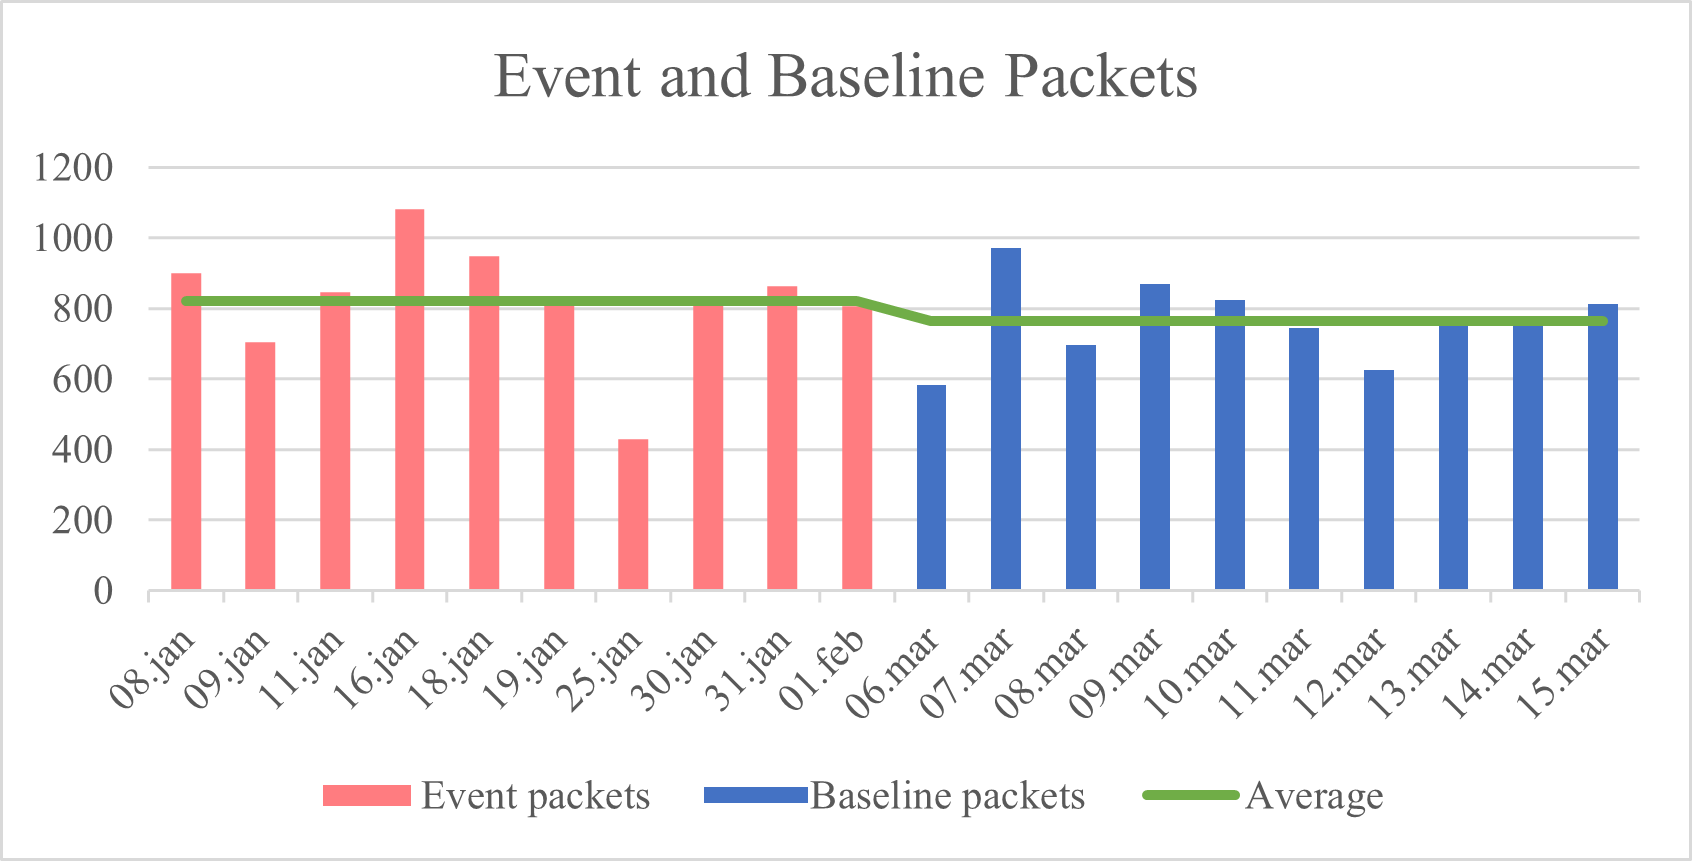
\includegraphics[width=1\hsize]{figures/Netatmo_Cooking_Calculations_Packets.png} 
    \end{subfigure}
    \begin{subfigure}{1\textwidth}
        \centering
        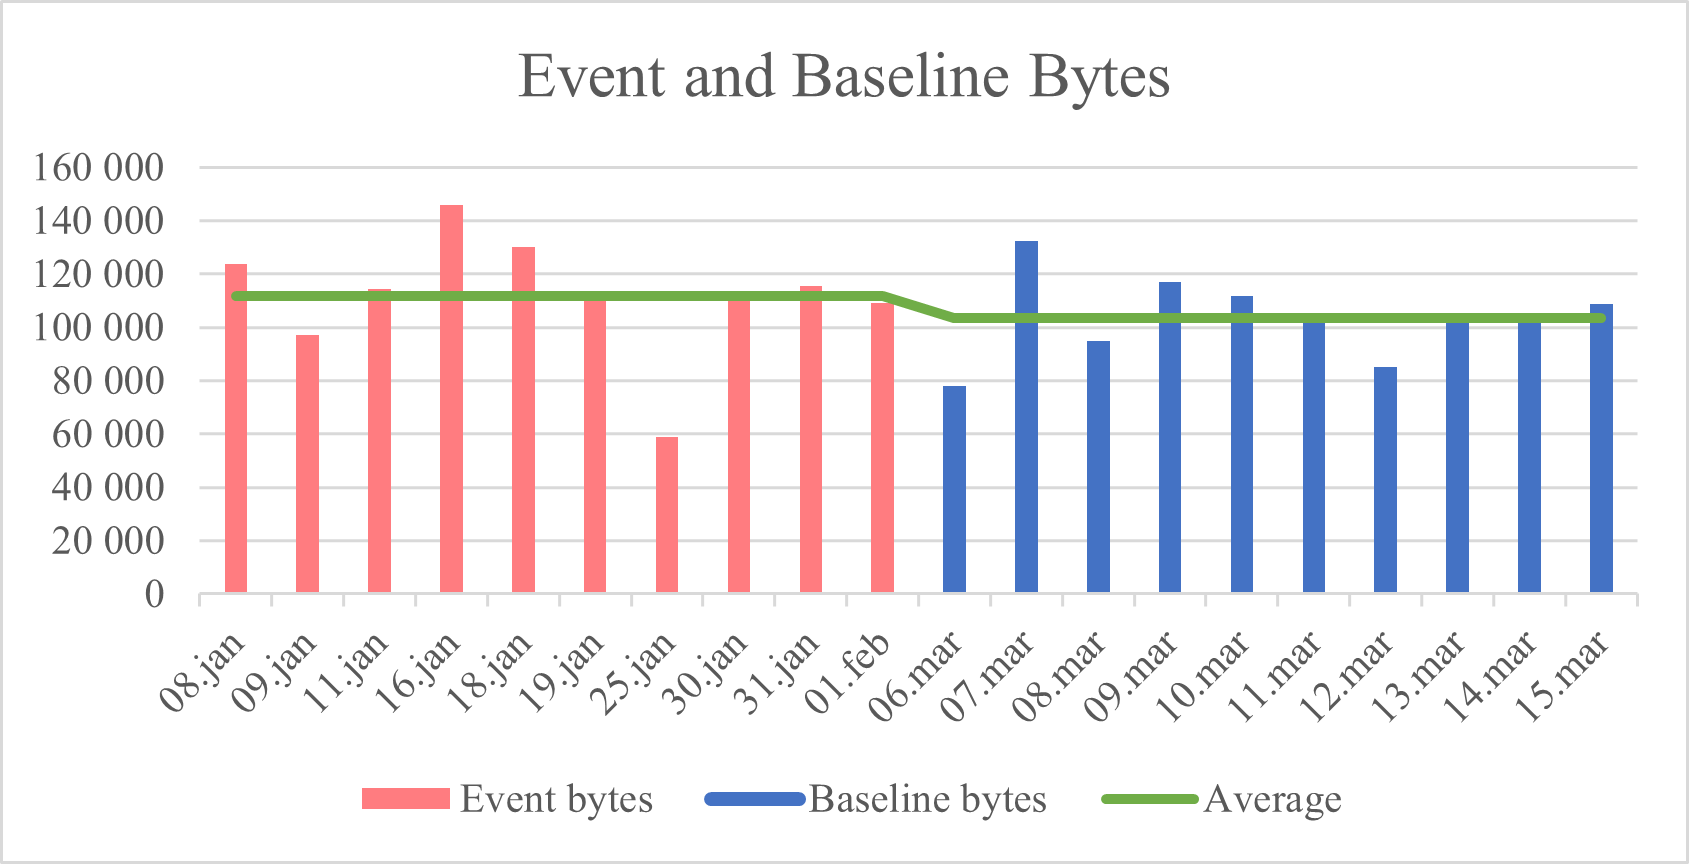
\includegraphics[width=1\hsize]{figures/Netatmo_Cooking_Calculations_Bytes.png} 
    \end{subfigure}
    \caption{Netatmo: Graphical presentation of cooking calculations with packets and bytes, including average value extracted from Table \ref{tab:NetatmoCookingCalculations}}
    \label{fig:NetatmoCookingCalculations}
\end{figure}

\begin{figure}[H]
    \begin{subfigure}[b]{0.47\textwidth}
        \centering
        \tcbincludegraphics[size=fbox,width=1.1\hsize,colframe=red]{figures/Netatmo_Cooking_Packets_08.01.png}
    \end{subfigure}
    \begin{subfigure}[b]{0.47\textwidth}
        \centering
        \tcbincludegraphics[size=fbox,width=1.1\hsize, colframe=blue]{figures/Netatmo_Cooking_Baseline_Packets_06.03.png}
    \end{subfigure}
    \begin{subfigure}[b]{0.47\textwidth}
        \centering
        \tcbincludegraphics[size=fbox,width=1.1\hsize,colframe=red]{figures/Netatmo_Cooking_Packets_09.01.png}
    \end{subfigure}
    \begin{subfigure}[b]{0.47\textwidth}
        \centering
        \tcbincludegraphics[size=fbox,width=1.1\hsize,colframe=blue]{figures/Netatmo_Cooking_Baseline_Packets_07.03.png}
    \end{subfigure}
    \begin{subfigure}[b]{0.47\textwidth}
        \centering
        \tcbincludegraphics[size=fbox,width=1.1\hsize,colframe=red]{figures/Netatmo_Cooking_Packets_11.01.png}
    \end{subfigure}
    \begin{subfigure}[b]{0.47\textwidth}
        \centering
        \tcbincludegraphics[size=fbox,width=1.1\hsize,colframe=blue]{figures/Netatmo_Cooking_Baseline_Packets_08.03.png}
    \end{subfigure}
    \begin{subfigure}[b]{0.47\textwidth}
        \centering
        \tcbincludegraphics[size=fbox,width=1.1\hsize,colframe=red]{figures/Netatmo_Cooking_Packets_16.01.png}
    \end{subfigure}
    \begin{subfigure}[b]{0.47\textwidth}
        \centering
        \tcbincludegraphics[size=fbox,width=1.1\hsize,colframe=blue]{figures/Netatmo_Cooking_Baseline_Packets_09.03.png}
    \end{subfigure}
    \begin{subfigure}[b]{0.47\textwidth}
        \centering
        \tcbincludegraphics[size=fbox,width=1.1\hsize,colframe=red]{figures/Netatmo_Cooking_Packets_18.01.png}
    \end{subfigure}
    \begin{subfigure}[b]{0.47\textwidth}
        \centering
        \tcbincludegraphics[size=fbox,width=1.1\hsize,colframe=blue]{figures/Netatmo_Cooking_Baseline_Packets_10.03.png}
    \end{subfigure}
        \begin{subfigure}[b]{0.47\textwidth}
        \centering
        \tcbincludegraphics[size=fbox,width=1.1\hsize,colframe=red]{figures/Netatmo_Cooking_Packets_19.01.png}
    \end{subfigure}
    \begin{subfigure}[b]{0.47\textwidth}
        \centering
        \tcbincludegraphics[size=fbox,width=1.1\hsize,colframe=blue]{figures/Netatmo_Cooking_Baseline_Packets_11.03.png}
    \end{subfigure}
    \begin{subfigure}[b]{0.47\textwidth}
        \centering
        \tcbincludegraphics[size=fbox,width=1.1\hsize,colframe=red]{figures/Netatmo_Cooking_Packets_25.01.png}
    \end{subfigure}
    \hspace{0.6cm}
    \begin{subfigure}[b]{0.47\textwidth}
    \centering
        \tcbincludegraphics[size=fbox,width=1.1\hsize,colframe=blue]{figures/Netatmo_Cooking_Baseline_Packets_12.03.png}
        \end{subfigure}
    \caption{Netatmo: Graphs from cooking events shown in packets with events in red and baseline in blue}
    \label{fig:NetatmoCookingPackets1}
\end{figure}

\begin{figure}[H]
    \begin{subfigure}[b]{0.45\textwidth}
        \centering
        \tcbincludegraphics[size=fbox,width=1.1\hsize,colframe=red]{figures/Netatmo_Cooking_Packets_30.01.png}
    \end{subfigure}
    \begin{subfigure}[b]{0.45\textwidth}
        \centering
        \tcbincludegraphics[size=fbox,width=1.1\hsize, colframe=blue]{figures/Netatmo_Cooking_Baseline_Packets_13.03.png}
    \end{subfigure}
    \begin{subfigure}[b]{0.45\textwidth}
        \centering
        \tcbincludegraphics[size=fbox,width=1.1\hsize,colframe=red]{figures/Netatmo_Cooking_Packets_31.01.png}
    \end{subfigure}
    \begin{subfigure}[b]{0.45\textwidth}
        \centering
        \tcbincludegraphics[size=fbox,width=1.1\hsize,colframe=blue]{figures/Netatmo_Cooking_Baseline_Packets_14.03.png}
    \end{subfigure}
    \begin{subfigure}[b]{0.45\textwidth}
        \centering
        \tcbincludegraphics[size=fbox,width=1.1\hsize,colframe=red]{figures/Netatmo_Cooking_Packets_01.02.png}
    \end{subfigure}
    \hspace{1.1cm}
    \begin{subfigure}[b]{0.45\textwidth}
        \centering
        \tcbincludegraphics[size=fbox,width=1.1\hsize,colframe=blue]{figures/Netatmo_Cooking_Baseline_Packets_15.03.png}
    \end{subfigure}
    \caption{Netatmo: Continuing from Figure \ref{fig:NetatmoCookingPackets1}}
    \label{fig:NetatmoCookingPackets2}
\end{figure}

\begin{figure}[H]
    \begin{subfigure}[b]{0.45\textwidth}
        \centering
        \tcbincludegraphics[size=fbox,width=1.1\hsize,colframe=red]{figures/Netatmo_Cooking_Bytes_30.01.png}
    \end{subfigure}
    \begin{subfigure}[b]{0.45\textwidth}
        \centering
        \tcbincludegraphics[size=fbox,width=1.1\hsize, colframe=blue]{figures/Netatmo_Cooking_Baseline_Bytes_13.03.png}
    \end{subfigure}
    \begin{subfigure}[b]{0.45\textwidth}
        \centering
        \tcbincludegraphics[size=fbox,width=1.1\hsize,colframe=red]{figures/Netatmo_Cooking_Bytes_31.01.png}
    \end{subfigure}
    \begin{subfigure}[b]{0.45\textwidth}
        \centering
        \tcbincludegraphics[size=fbox,width=1.1\hsize,colframe=blue]{figures/Netatmo_Cooking_Baseline_Bytes_14.03.png}
    \end{subfigure}
    \begin{subfigure}[b]{0.45\textwidth}
        \centering
        \tcbincludegraphics[size=fbox,width=1.1\hsize,colframe=red]{figures/Netatmo_Cooking_Bytes_01.02.png}
    \end{subfigure}
    \hspace{1.1cm}
    \begin{subfigure}[b]{0.45\textwidth}
        \centering
        \tcbincludegraphics[size=fbox,width=1.1\hsize,colframe=blue]{figures/Netatmo_Cooking_Baseline_Bytes_15.03.png}
    \end{subfigure}
    \caption{Netatmo: First graphs from Figure \ref{fig:NetatmoCookingBytes2}}
    \label{fig:NetatmoCookingBytes1}
\end{figure}

\begin{figure}[H]
    \begin{subfigure}[b]{0.47\textwidth}
        \centering
        \tcbincludegraphics[size=fbox,width=1.1\hsize,colframe=red]{figures/Netatmo_Cooking_Bytes_08.01.png}
    \end{subfigure}
    \begin{subfigure}[b]{0.47\textwidth}
        \centering
        \tcbincludegraphics[size=fbox,width=1.1\hsize,colframe=blue]{figures/Netatmo_Cooking_Baseline_Bytes_06.03.png}
    \end{subfigure}
    \begin{subfigure}[b]{0.47\textwidth}
        \centering
        \tcbincludegraphics[size=fbox,width=1.1\hsize,colframe=red]{figures/Netatmo_Cooking_Bytes_09.01.png}
    \end{subfigure}
    \begin{subfigure}[b]{0.47\textwidth}
        \centering
        \tcbincludegraphics[size=fbox,width=1.1\hsize,colframe=blue]{figures/Netatmo_Cooking_Baseline_Bytes_07.03.png}
    \end{subfigure}
    \begin{subfigure}[b]{0.47\textwidth}
        \centering
        \tcbincludegraphics[size=fbox,width=1.1\hsize,colframe=red]{figures/Netatmo_Cooking_Bytes_11.01.png}
    \end{subfigure}
    \begin{subfigure}[b]{0.47\textwidth}
        \centering
        \tcbincludegraphics[size=fbox,width=1.1\hsize,colframe=blue]{figures/Netatmo_Cooking_Baseline_Bytes_08.03.png}
    \end{subfigure}
    \begin{subfigure}[b]{0.47\textwidth}
        \centering
        \tcbincludegraphics[size=fbox,width=1.1\hsize,colframe=red]{figures/Netatmo_Cooking_Bytes_16.01.png}
    \end{subfigure}
    \begin{subfigure}[b]{0.47\textwidth}
        \centering
        \tcbincludegraphics[size=fbox,width=1.1\hsize,colframe=blue]{figures/Netatmo_Cooking_Baseline_Bytes_09.03.png}
    \end{subfigure}
    \begin{subfigure}[b]{0.47\textwidth}
        \centering
        \tcbincludegraphics[size=fbox,width=1.1\hsize,colframe=red]{figures/Netatmo_Cooking_Bytes_18.01.png}
    \end{subfigure}
    \begin{subfigure}[b]{0.47\textwidth}
        \centering
        \tcbincludegraphics[size=fbox,width=1.1\hsize,colframe=blue]{figures/Netatmo_Cooking_Baseline_Bytes_10.03.png}
    \end{subfigure}
        \begin{subfigure}[b]{0.47\textwidth}
        \centering
        \tcbincludegraphics[size=fbox,width=1.1\hsize,colframe=red]{figures/Netatmo_Cooking_Bytes_19.01.png}
    \end{subfigure}
    \begin{subfigure}[b]{0.47\textwidth}
        \centering
        \tcbincludegraphics[size=fbox,width=1.1\hsize,colframe=blue]{figures/Netatmo_Cooking_Baseline_Bytes_11.03.png}
    \end{subfigure}
    \begin{subfigure}[b]{0.47\textwidth}
        \centering
        \tcbincludegraphics[size=fbox,width=1.1\hsize,colframe=red]{figures/Netatmo_Cooking_Bytes_25.01.png}
    \end{subfigure}
    \hspace{0.6cm}
    \begin{subfigure}[b]{0.47\textwidth}
    \centering
        \tcbincludegraphics[size=fbox,width=1.1\hsize,colframe=blue]{figures/Netatmo_Cooking_Baseline_Bytes_12.03.png}
        \end{subfigure}
    \caption{Netatmo: Graphs from cooking events shown in bytes with events in red and baseline in blue}
    \label{fig:NetatmoCookingBytes2}
\end{figure}

Table \ref{tab:NetatmoCookingCalculations} shows that the calculations varies a lot for each event. Packets varies from 403 to 1,082 and bytes from 58,926 to 146,001. Compared to the baseline calculations, which also varies with 584 packets as the smallest number to 972 to the highest amount of packets during the time. For bytes it varies from 77,780 to 132,406 bytes. The biggest packets from both the events and the baseline is mainly 407 bytes, with a few exceptions for both. The average values for both packets and bytes are similar to each other for the events and baseline. The average value for biggest packet are almost the same as the values for each day are almost the same as shown in Table in \ref{tab:NetatmoCookingCalculations} and \ref{tab:NetatmoBaselineCookingCalculations}. The standard deviation for all categories are a bit higher for the events than the baseline. Overall, the graphs in Figure \ref{fig:NetatmoCookingCalculations} shows that the calculation of the traffic from the events, do not differ significantly from the baseline standard traffic.
\\\\
The same result is further confirmed in the graphs in Figure \ref{fig:NetatmoCookingPackets1} and \ref{fig:NetatmoCookingPackets2} for packets and \ref{fig:NetatmoCookingBytes1} and \ref{fig:NetatmoCookingBytes2} for bytes. The graphs for events in red do not follow a specific pattern compared to the baseline traffic in blue. 

\newpage
\subsection{Mill Sense}
The results from the cooking events for Mill are presented with both numerical values in tables and graphs and in figures where traffic pattern can be analyzed. Table \ref{tab:MillCookingCalculations} presents the calculations from the event traffic with packets, bytes and biggest packet. The same calculations have been made on the baseline traffic. in Table \ref{tab:MillBaselineCookingCalculations}. Table \ref{tab:MillComparingBaselineAndCookingCalculations} compares the average and standard deviation values for the event and baseline traffic. The calculations from these three tables are graphically presented in Figure \ref{fig:MillCookingCalculations} where packets and bytes from the event and baseline traffic are included with the average value for each of them. The traffic pattern of the events and baseline are presented in Figure \ref{fig:MillCookingPackets1} and \ref{fig:MillCookingPackets2} for packets and in Figure \ref{fig:MillCookingBytes1} and \ref{fig:MillCookingBytes2} for bytes. In these figures, all graphs have the same minimum and maximum values on the y- and x-axis to be comparable. The graphs created from the different events are placed on the left side of the figure and marked in red, while the baseline is placed on the right side of the figure and marked in blue. 

\begin{table}[H]
    \centering
    \caption{Mill Cooking Calculations}
    \begin{tabular}{|l|l|l|l|l|l|}
    \hline
        \textbf{Events} & \textbf{Packets} & \textbf{Bytes} & \textbf{Biggest packet} \\ \hline
        08.jan & 8,875  & 1,097,786 & 456 bytes   \\ \hline
        09.jan & 7,948  & 1,057,936 & 456 bytes   \\ \hline
        11.jan & 10,222 & 1,310,644 & 456 bytes   \\ \hline
        16.jan & 10,014 & 1,358,615 & 1,353 bytes \\ \hline
        18.jan & 9,185  & 1,137,586 & 456 bytes   \\ \hline
        19.jan & 8,306  & 1,062,743 & 1,593 bytes \\ \hline
        25.jan & 8,246  & 1,033,976 & 1,583 bytes \\ \hline
        30.jan & 11,826 & 1,357,595 & 1,343 bytes  \\ \hline
        31.jan & 10,464 & 1,205,006 & 456 bytes \\ \hline
        01.feb & 10,124 & 1,219,206 & 456 bytes \\ \hline
    \end{tabular}
    \label{tab:MillCookingCalculations}
\end{table}

\begin{table}[H]
    \centering
    \caption{Mill Baseline Cooking Calculations}
    \begin{tabular}{|l|l|l|l|l|l|}
    \hline
        \textbf{Baseline} & \textbf{Packets} & \textbf{Bytes} & \textbf{Biggest packet} \\ \hline
        06.mar & 8,808  & 835,070   & 426 bytes \\ \hline
        07.mar & 9,310  & 940,428   & 1,353 bytes \\ \hline
        08.mar & 8,930  & 904,598   & 1,343 bytes \\ \hline
        09.mar & 10,675 & 1,046,076 & 456 bytes \\ \hline
        10.mar & 6,989  & 774,986   & 1,573 bytes \\ \hline
        11.mar & 9,983  & 1,107,006 & 1,273 bytes \\ \hline
        12.mar & 10,740 & 1,033,467 & 456 bytes \\ \hline
        13.mar & 8,134  & 826,038   & 426 bytes \\ \hline
        14.mar & 9,090  & 969,576   & 1,573 bytes \\ \hline
        15.mar & 6,539  & 740,761   & 429 bytes \\ \hline
    \end{tabular}
    \label{tab:MillBaselineCookingCalculations}
\end{table}

\begin{table}[H]
    \centering
    \caption{Comparing Cooking and Baseline Calculations for Mill}
    \begin{tabular}{c|l|l|l|l|}
        \cline{2-5}
        \multicolumn{1}{l|}{}                                              & \textbf{Type} & \textbf{Packets} & \textbf{Bytes} & \textbf{Biggest packet} \\ \hline
        \multicolumn{1}{|c|}{\multirow{2}{*}{\textbf{Average}}}            & Event         & 9,521              & 1,184,109       & 861 bytes               \\ \cline{2-5} 
        \multicolumn{1}{|c|}{}                                             & Baseline      & 8,920              & 917,801         & 931 bytes                \\ \hline
        \multicolumn{1}{|c|}{\multirow{2}{*}{\textbf{Standard deviation}}} & Event         & 1,221              & 125,182         & 529 bytes                 \\ \cline{2-5} 
        \multicolumn{1}{|c|}{}                                             & Baseline      & 1,404               & 122,928       &  527 bytes               \\ \hline          
    \end{tabular}
    \label{tab:MillComparingBaselineAndCookingCalculations}
\end{table}

\begin{figure}[H]
    \centering
    \begin{subfigure}{1\textwidth}
        \centering
        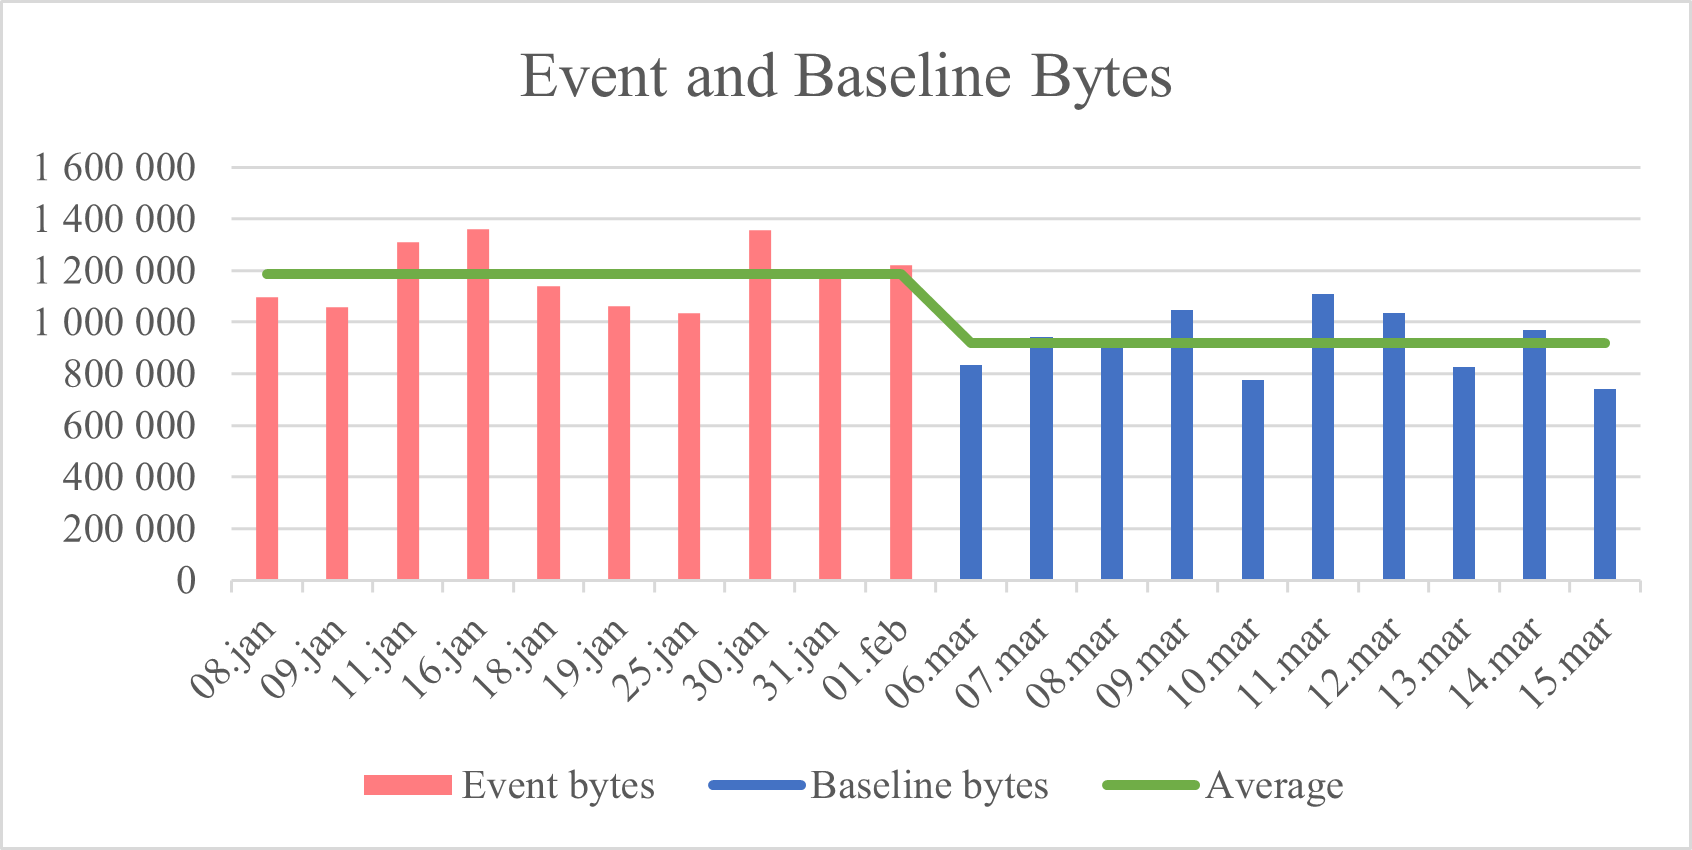
\includegraphics[width=1\hsize]{figures/Mill_Cooking_Calculations_Bytes.png} 
    \end{subfigure}
    \begin{subfigure}{1\textwidth}
        \centering
        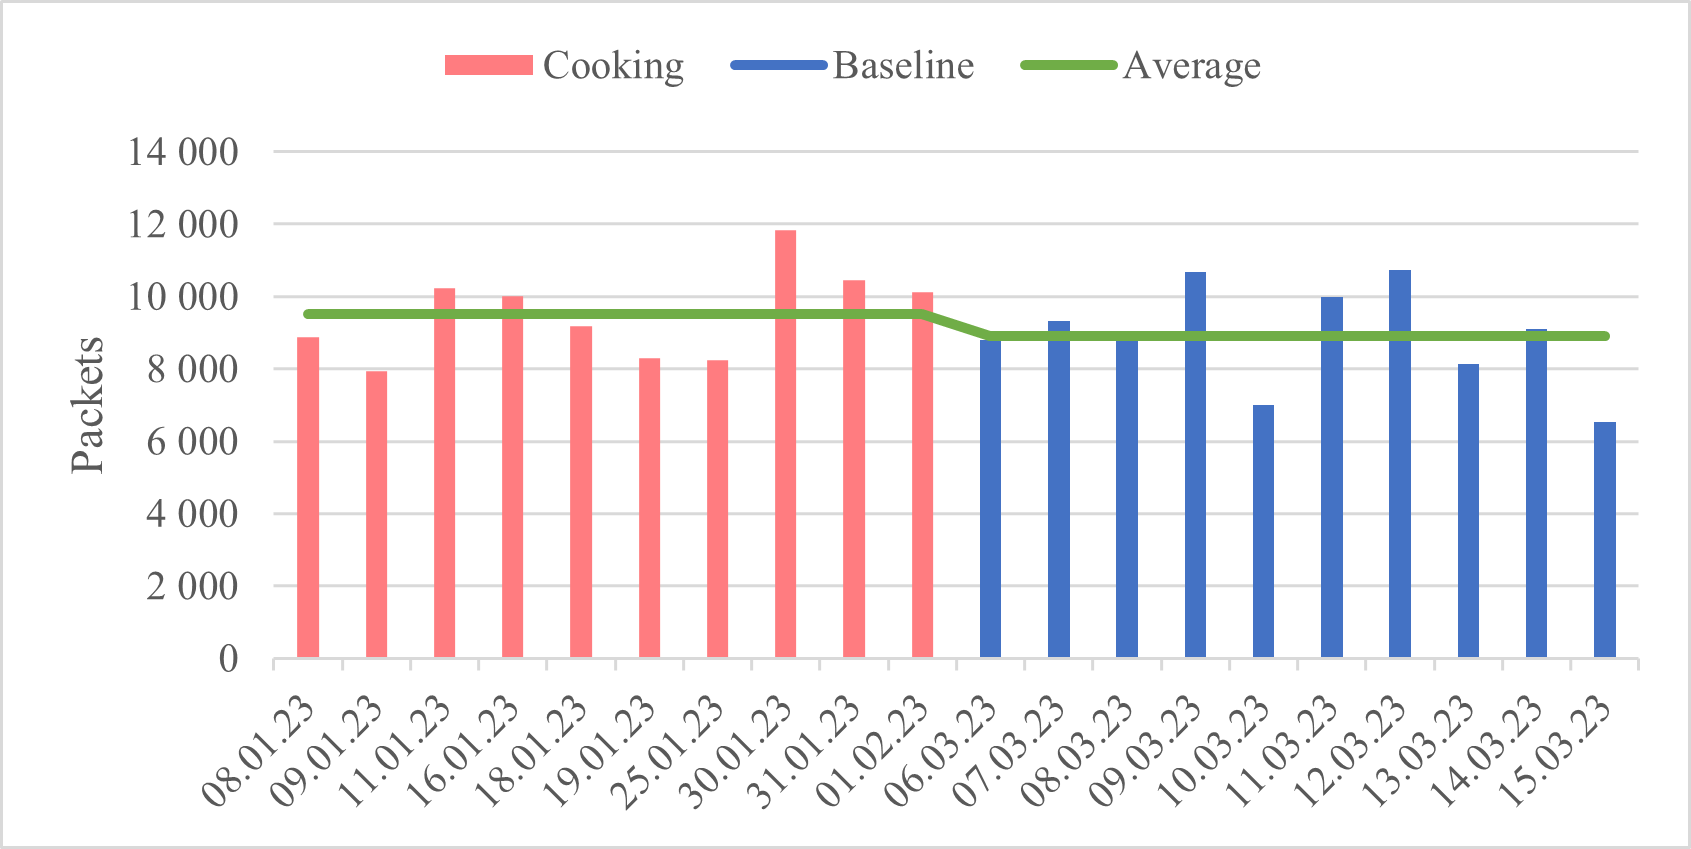
\includegraphics[width=1\hsize]{figures/Mill_Cooking_Calculations_Packets.png} 
    \end{subfigure}
    \caption{Cooking Calculations for Mill}
    \label{fig:MillCookingCalculations}
\end{figure}

\begin{figure}[H]
    \begin{subfigure}[b]{0.47\textwidth}
        \centering
        \tcbincludegraphics[size=fbox,width=1.1\hsize,colframe=red]{figures/Mill_Cooking_Packets_08.01.png}
    \end{subfigure}
    \begin{subfigure}[b]{0.47\textwidth}
        \centering
        \tcbincludegraphics[size=fbox,width=1.1\hsize, colframe=blue]{figures/Mill_Cooking_Baseline_Packets_06.03.png}
    \end{subfigure}
    \begin{subfigure}[b]{0.47\textwidth}
        \centering
        \tcbincludegraphics[size=fbox,width=1.1\hsize,colframe=red]{figures/Mill_Cooking_Packets_09.01.png}
    \end{subfigure}
    \begin{subfigure}[b]{0.47\textwidth}
        \centering
        \tcbincludegraphics[size=fbox,width=1.1\hsize,colframe=blue]{figures/Mill_Cooking_Baseline_Packets_07.03.png}
    \end{subfigure}
    \begin{subfigure}[b]{0.47\textwidth}
        \centering
        \tcbincludegraphics[size=fbox,width=1.1\hsize,colframe=red]{figures/Mill_Cooking_Packets_11.01.png}
    \end{subfigure}
    \begin{subfigure}[b]{0.47\textwidth}
        \centering
        \tcbincludegraphics[size=fbox,width=1.1\hsize,colframe=blue]{figures/Mill_Cooking_Baseline_Packets_08.03.png}
    \end{subfigure}
    \begin{subfigure}[b]{0.47\textwidth}
        \centering
        \tcbincludegraphics[size=fbox,width=1.1\hsize,colframe=red]{figures/Mill_Cooking_Packets_16.01.png}
    \end{subfigure}
    \begin{subfigure}[b]{0.47\textwidth}
        \centering
        \tcbincludegraphics[size=fbox,width=1.1\hsize,colframe=blue]{figures/Mill_Cooking_Baseline_Packets_09.03.png}
    \end{subfigure}
    \begin{subfigure}[b]{0.47\textwidth}
        \centering
        \tcbincludegraphics[size=fbox,width=1.1\hsize,colframe=red]{figures/Mill_Cooking_Packets_18.01.png}
    \end{subfigure}
    \begin{subfigure}[b]{0.47\textwidth}
        \centering
        \tcbincludegraphics[size=fbox,width=1.1\hsize,colframe=blue]{figures/Mill_Cooking_Baseline_Packets_10.03.png}
    \end{subfigure}
        \begin{subfigure}[b]{0.47\textwidth}
        \centering
        \tcbincludegraphics[size=fbox,width=1.1\hsize,colframe=red]{figures/Mill_Cooking_Packets_19.01.png}
    \end{subfigure}
    \begin{subfigure}[b]{0.47\textwidth}
        \centering
        \tcbincludegraphics[size=fbox,width=1.1\hsize,colframe=blue]{figures/Mill_Cooking_Baseline_Packets_11.03.png}
    \end{subfigure}
    \begin{subfigure}[b]{0.47\textwidth}
        \centering
        \tcbincludegraphics[size=fbox,width=1.1\hsize,colframe=red]{figures/Mill_Cooking_Packets_25.01.png}
    \end{subfigure}
    \hspace{0.6cm}
    \begin{subfigure}[b]{0.47\textwidth}
    \centering
        \tcbincludegraphics[size=fbox,width=1.1\hsize,colframe=blue]{figures/Mill_Cooking_Baseline_Packets_12.03.png}
        \end{subfigure}
    \caption{Mill: Graphs from cooking events shown in packets with events in red and baseline in blue}
    \label{fig:MillCookingPackets1}
\end{figure}

\begin{figure}[H]
    \begin{subfigure}[b]{0.45\textwidth}
        \centering
        \tcbincludegraphics[size=fbox,width=1.1\hsize,colframe=red]{figures/Mill_Cooking_Packets_30.01.png}
    \end{subfigure}
    \begin{subfigure}[b]{0.45\textwidth}
        \centering
        \tcbincludegraphics[size=fbox,width=1.1\hsize, colframe=blue]{figures/Mill_Cooking_Baseline_Packets_13.03.png}
    \end{subfigure}
    \begin{subfigure}[b]{0.45\textwidth}
        \centering
        \tcbincludegraphics[size=fbox,width=1.1\hsize,colframe=red]{figures/Mill_Cooking_Packets_31.01.png}
    \end{subfigure}
    \begin{subfigure}[b]{0.45\textwidth}
        \centering
        \tcbincludegraphics[size=fbox,width=1.1\hsize,colframe=blue]{figures/Mill_Cooking_Baseline_Packets_14.03.png}
    \end{subfigure}
    \begin{subfigure}[b]{0.45\textwidth}
        \centering
        \tcbincludegraphics[size=fbox,width=1.1\hsize,colframe=red]{figures/Mill_Cooking_Packets_01.02.png}
    \end{subfigure}
    \hspace{1.1cm}
    \begin{subfigure}[b]{0.45\textwidth}
        \centering
        \tcbincludegraphics[size=fbox,width=1.1\hsize,colframe=blue]{figures/Mill_Cooking_Baseline_Packets_15.03.png}
    \end{subfigure}
    \caption{Mill: Continuing from Figure \ref{fig:MillCookingPackets1}}
    \label{fig:MillCookingPackets2}
\end{figure}

\begin{figure}[H]
    \begin{subfigure}[b]{0.45\textwidth}
        \centering
        \tcbincludegraphics[size=fbox,width=1.1\hsize,colframe=red]{figures/Mill_Cooking_Bytes_30.01.png}
    \end{subfigure}
    \begin{subfigure}[b]{0.45\textwidth}
        \centering
        \tcbincludegraphics[size=fbox,width=1.1\hsize, colframe=blue]{figures/Mill_Cooking_Baseline_Bytes_13.03.png}
    \end{subfigure}
    \begin{subfigure}[b]{0.45\textwidth}
        \centering
        \tcbincludegraphics[size=fbox,width=1.1\hsize,colframe=red]{figures/Mill_Cooking_Bytes_31.01.png}
    \end{subfigure}
    \begin{subfigure}[b]{0.45\textwidth}
        \centering
        \tcbincludegraphics[size=fbox,width=1.1\hsize,colframe=blue]{figures/Mill_Cooking_Baseline_Bytes_14.03.png}
    \end{subfigure}
    \begin{subfigure}[b]{0.45\textwidth}
        \centering
        \tcbincludegraphics[size=fbox,width=1.1\hsize,colframe=red]{figures/Mill_Cooking_Bytes_01.02.png}
    \end{subfigure}
    \hspace{1.1cm}
    \begin{subfigure}[b]{0.45\textwidth}
        \centering
        \tcbincludegraphics[size=fbox,width=1.1\hsize,colframe=blue]{figures/Mill_Cooking_Baseline_Bytes_15.03.png}
    \end{subfigure}
    \caption{Mill: First graphs from Figure \ref{fig:MillCookingBytes2}}
    \label{fig:MillCookingBytes1}
\end{figure}

\begin{figure}[H]
    \begin{subfigure}[b]{0.47\textwidth}
        \centering
        \tcbincludegraphics[size=fbox,width=1.1\hsize,colframe=red]{figures/Mill_Cooking_Bytes_08.01.png}
    \end{subfigure}
    \begin{subfigure}[b]{0.47\textwidth}
        \centering
        \tcbincludegraphics[size=fbox,width=1.1\hsize,colframe=blue]{figures/Mill_Cooking_Baseline_Bytes_06.03.png}
    \end{subfigure}
    \begin{subfigure}[b]{0.47\textwidth}
        \centering
        \tcbincludegraphics[size=fbox,width=1.1\hsize,colframe=red]{figures/Mill_Cooking_Bytes_09.01.png}
    \end{subfigure}
    \begin{subfigure}[b]{0.47\textwidth}
        \centering
        \tcbincludegraphics[size=fbox,width=1.1\hsize,colframe=blue]{figures/Mill_Cooking_Baseline_Bytes_07.03.png}
    \end{subfigure}
    \begin{subfigure}[b]{0.47\textwidth}
        \centering
        \tcbincludegraphics[size=fbox,width=1.1\hsize,colframe=red]{figures/Mill_Cooking_Bytes_11.01.png}
    \end{subfigure}
    \begin{subfigure}[b]{0.47\textwidth}
        \centering
        \tcbincludegraphics[size=fbox,width=1.1\hsize,colframe=blue]{figures/Mill_Cooking_Baseline_Bytes_08.03.png}
    \end{subfigure}
    \begin{subfigure}[b]{0.47\textwidth}
        \centering
        \tcbincludegraphics[size=fbox,width=1.1\hsize,colframe=red]{figures/Mill_Cooking_Bytes_16.01.png}
    \end{subfigure}
    \begin{subfigure}[b]{0.47\textwidth}
        \centering
        \tcbincludegraphics[size=fbox,width=1.1\hsize,colframe=blue]{figures/Mill_Cooking_Baseline_Bytes_09.03.png}
    \end{subfigure}
    \begin{subfigure}[b]{0.47\textwidth}
        \centering
        \tcbincludegraphics[size=fbox,width=1.1\hsize,colframe=red]{figures/Mill_Cooking_Bytes_18.01.png}
    \end{subfigure}
    \begin{subfigure}[b]{0.47\textwidth}
        \centering
        \tcbincludegraphics[size=fbox,width=1.1\hsize,colframe=blue]{figures/Mill_Cooking_Baseline_Bytes_10.03.png}
    \end{subfigure}
        \begin{subfigure}[b]{0.47\textwidth}
        \centering
        \tcbincludegraphics[size=fbox,width=1.1\hsize,colframe=red]{figures/Mill_Cooking_Bytes_19.01.png}
    \end{subfigure}
    \begin{subfigure}[b]{0.47\textwidth}
        \centering
        \tcbincludegraphics[size=fbox,width=1.1\hsize,colframe=blue]{figures/Mill_Cooking_Baseline_Bytes_11.03.png}
    \end{subfigure}
    \begin{subfigure}[b]{0.47\textwidth}
        \centering
        \tcbincludegraphics[size=fbox,width=1.1\hsize,colframe=red]{figures/Mill_Cooking_Bytes_25.01.png}
    \end{subfigure}
    \hspace{0.6cm}
    \begin{subfigure}[b]{0.47\textwidth}
    \centering
        \tcbincludegraphics[size=fbox,width=1.1\hsize,colframe=blue]{figures/Mill_Cooking_Baseline_Bytes_12.03.png}
        \end{subfigure}
    \caption{Mill: Graphs from cooking events shown in bytes with events in red and baseline in blue}
    \label{fig:MillCookingBytes2}
\end{figure}

Comparing Table \ref{tab:MillCookingCalculations} and \ref{tab:MillBaselineCookingCalculations} shows that the amount of packets sent to and from the device is around the same amount and not a significant difference between the two. The average values for packets in Table \ref{tab:MillComparingBaselineAndCookingCalculations} also shows that the values are similar to each other. For bytes, the calculations shows that when an event is ongoing, the overall values are higher than for standard baseline traffic. The comparison in Table \ref{tab:MillComparingBaselineAndCookingCalculations} shows that the average value for events are 266,308 bytes higher. The same is presented in Figure \ref{fig:MillCookingCalculations} where there are a bigger difference in bytes than packets in events and baseline traffic. For biggest packet sent, the same pattern is visible in both Table \ref{tab:MillCookingCalculations} and \ref{tab:MillBaselineCookingCalculations} where the packet sizes varies from around 450 bytes to 1,550 bytes for events and baseline traffic over the same time. 
\\\\
The graphs in Figure \ref{fig:MillCookingPackets1} and \ref{fig:MillCookingPackets2} for packets and Figure \ref{fig:MillCookingBytes1} and \ref{fig:MillCookingBytes2} for bytes does not show a significant change in traffic pattern from when an event is ongoing in the graphs marked in red and the standard traffic pattern from the baseline in the graphs marked in blue. The variations the calculations gave in bytes from the events and baseline is not very visible in the graphs as they both vary a lot. However, knowing that more bytes are sent during the events, it is possible to see that more of the event graphs have higher spikes than the baseline, but this is not applicable for all events. 

\newpage
\subsection{Nedis}
In Test Case 1: Cooking for the device Nedis, tables with numerical calculations are presented together with graphs of the traffic flow. In Table \ref{tab:NedisCookingCalculations} the total amount of packets and bytes including the biggest packet during the event are presented for each of the 10 cooking events. Table \ref{tab:NedisBaselineCookingCalculations} the same values are presented, but in regards of the baseline days. Table \ref{tab:NedisComparingBaselineAndCookingCalculations} compares the average values and standard deviation from the events and baseline for packets, bytes and biggest packet. Figure \ref{fig:NedisCookingCalculations} presents the calculations from Table \ref{tab:NedisCookingCalculations}, \ref{tab:NedisBaselineCookingCalculations} and \ref{tab:NedisComparingBaselineAndCookingCalculations} with packets and bytes together with the average value for both the event and baseline traffic to easier compare it. The graphical presentation of the traffic patterns during event are presented in Figure \ref{fig:NedisCookingPackets1} and \ref{fig:NedisCookingPackets2} for packets and in Figure \ref{fig:NedisCookingBytes1} and \ref{fig:NedisCookingBytes2} for bytes. In these figures, the corresponding graphs from the baseline traffic is also included to look for traffic changes during the events. In these figures, the graphs for events are placed on the left side of the figure and marked in red, while the baseline graphs are placed on the right side and marked in blue.    

\begin{table}[H]
\centering
\caption{Nedis Cooking Calculations}
\label{tab:NedisCookingCalculations}
    \begin{tabular}{|l|l|l|l|}
        \hline
        \textbf{Events}    & \textbf{Packets} & \textbf{Bytes}     & \textbf{Biggest packet} \\ \hline
        08.jan             & 24,494           & 3,318,519          & 485 bytes               \\ \hline
        09.jan             & 26,787           & 3,870,361          & 424 bytes               \\ \hline
        11.jan             & 24,381           & 3,550,947          & 424 bytes               \\ \hline
        16.jan             & 26,035           & 3,895,071          & 485 bytes               \\ \hline
        18.jan             & 25,398           & 3,233,845          & 424 bytes               \\ \hline
        19.jan             & 20,857           & 3,242,594          & 424 bytes               \\ \hline
        25.jan             & 24,233           & 3,095,693          & 424 bytes               \\ \hline
        30.jan             & 24,867           & 3,257,812          & 424 bytes               \\ \hline
        31.jan             & 23,882           & 3,179,117          & 424 bytes               \\ \hline
        01.feb             & 25,397           & 3,477,014          & 424 bytes               \\ \hline
    \end{tabular}
\end{table}

\begin{table}[H]
    \centering
    \caption{Nedis Baseline Cooking Calculations}
    \begin{tabular}{|l|l|l|l|l|l|}
    \hline
        \textbf{Baseline} & \textbf{Packets} & \textbf{Bytes} & \textbf{Biggest packet} \\ \hline
        06.mar & 13,014 & 1,413,457 & 421 bytes \\ \hline
        07.mar & 18,634 & 2,001,978 & 421 bytes \\ \hline
        08.mar & 18,643 & 2,019,872 & 421 bytes \\ \hline
        09.mar & 21,885 & 2,606,363 & 424 bytes \\ \hline
        10.mar & 17,956 & 2,326,898 & 424 bytes \\ \hline
        11.mar & 18,380 & 2,126,816 & 485 bytes \\ \hline
        12.mar & 10,728 & 1,312,915 & 421 bytes \\ \hline
        13.mar & 15,815 & 1,968,872 & 424 bytes \\ \hline
        14.mar & 15,926 & 1,878,449 & 341 bytes \\ \hline
        15.mar & 19,260 & 2,524,793 & 458 bytes \\ \hline
    \end{tabular}
    \label{tab:NedisBaselineCookingCalculations}
\end{table}

\begin{table}[H]
    \centering
    \caption{Comparing Cooking and Baseline Calculations for Nedis}
    \begin{tabular}{c|l|l|l|l|}
        \cline{2-5}
        \multicolumn{1}{l|}{}                                              & \textbf{Type} & \textbf{Packets} & \textbf{Bytes} & \textbf{Biggest packet} \\ \hline
        \multicolumn{1}{|c|}{\multirow{2}{*}{\textbf{Average}}}            & Event         & 24,633             & 3,412,097       & 436 bytes               \\ \cline{2-5} 
        \multicolumn{1}{|c|}{}                                             & Baseline      & 17,024             & 2,018,041       & 424 bytes                \\ \hline
        \multicolumn{1}{|c|}{\multirow{2}{*}{\textbf{Standard deviation}}} & Event         & 1,595              & 281,705         & 26 bytes                 \\ \cline{2-5} 
        \multicolumn{1}{|c|}{}                                             & Baseline      & 3,248              & 420,982         & 36 bytes               \\ \hline          
    \end{tabular}
    \label{tab:NedisComparingBaselineAndCookingCalculations}
\end{table}

\begin{figure}[H]
    \centering
    \begin{subfigure}{1\textwidth}
        \centering
        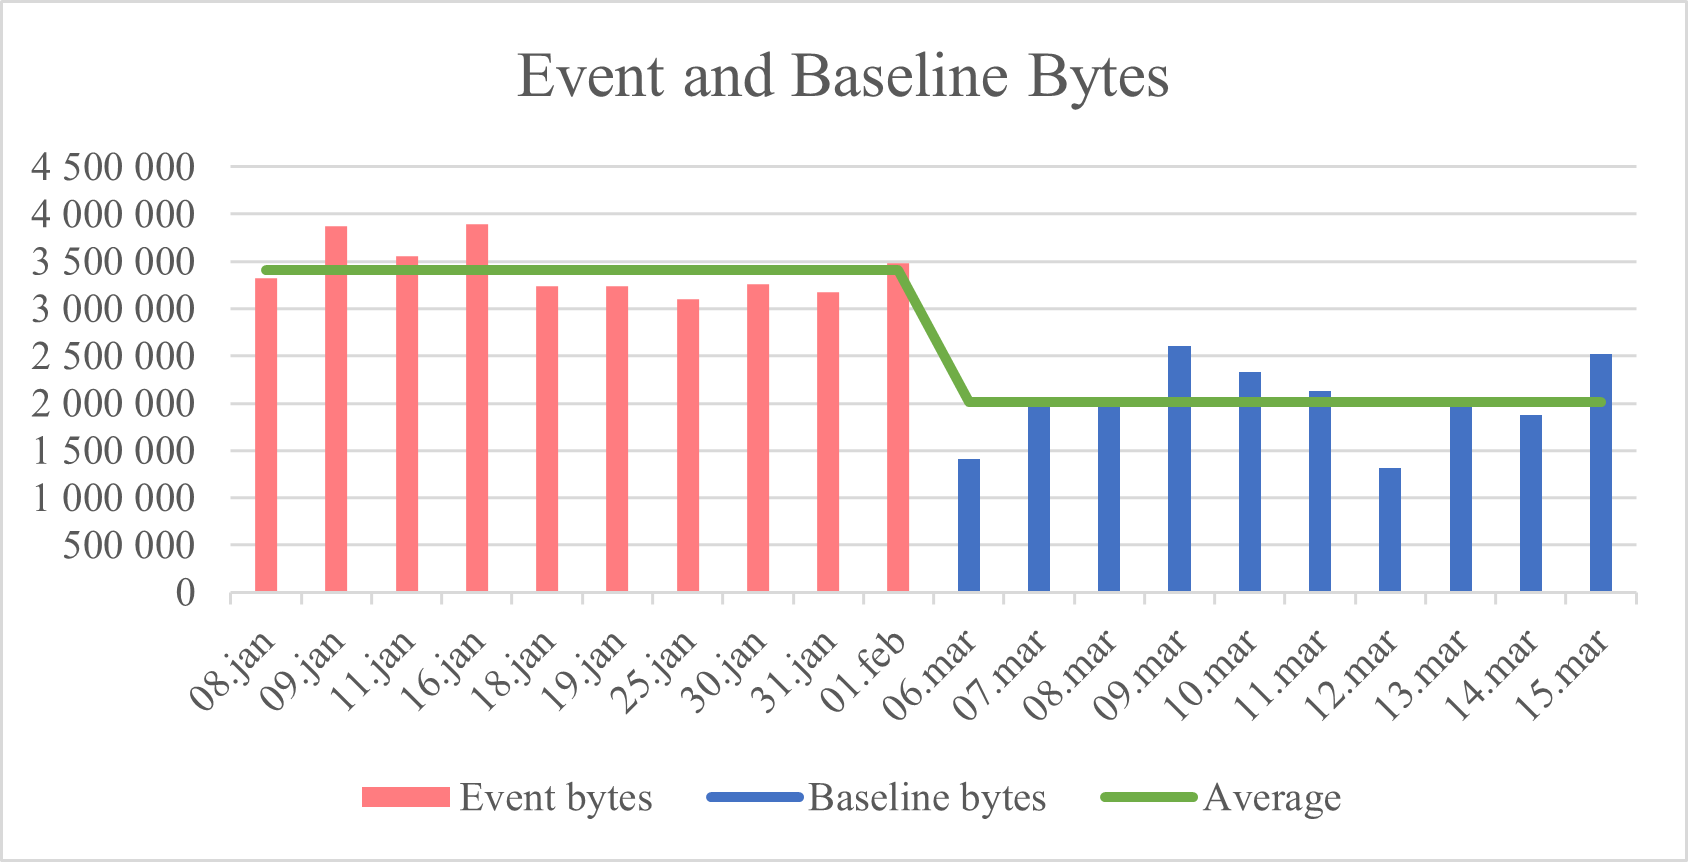
\includegraphics[width=1\hsize]{figures/Nedis_Cooking_Calculations_Bytes.png} 
    \end{subfigure}
    \begin{subfigure}{1\textwidth}
        \centering
        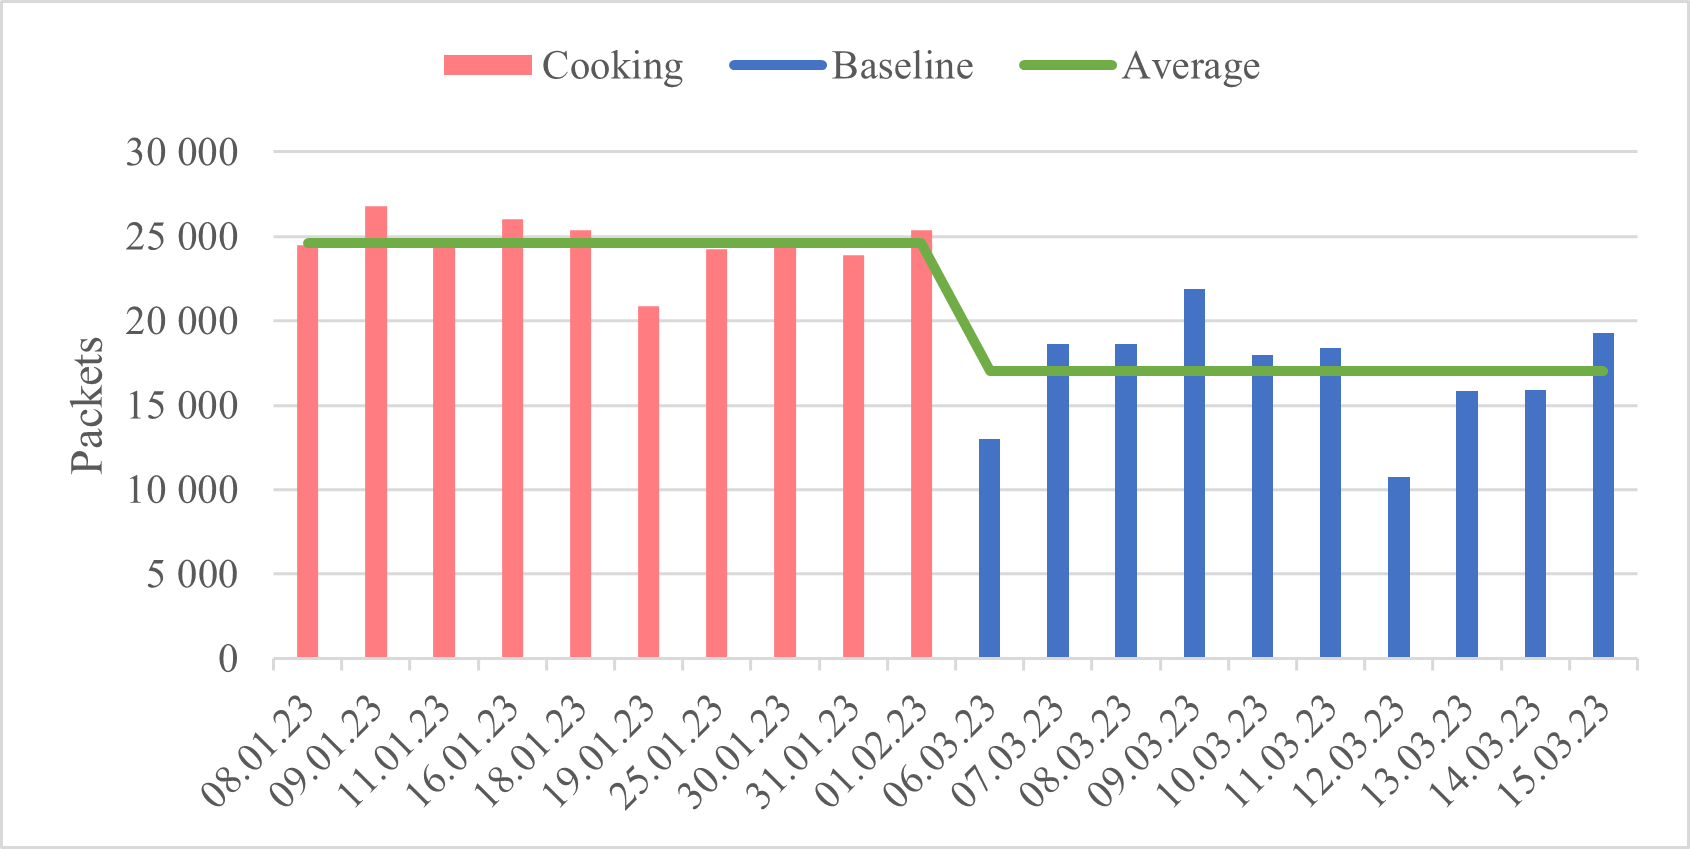
\includegraphics[width=1\hsize]{figures/Nedis_Cooking_Calculations_Packets.png} 
    \end{subfigure}
    \caption{Cooking Calculations for Nedis}
    \label{fig:NedisCookingCalculations}
\end{figure}

\begin{figure}[H]
    \begin{subfigure}[b]{0.47\textwidth}
        \centering
        \tcbincludegraphics[size=fbox,width=1.1\hsize,colframe=red]{figures/Nedis_Cooking_Packets_08.01.png}
    \end{subfigure}
    \begin{subfigure}[b]{0.47\textwidth}
        \centering
        \tcbincludegraphics[size=fbox,width=1.1\hsize, colframe=blue]{figures/Nedis_Cooking_Baseline_Packets_06.03.png}
    \end{subfigure}
    \begin{subfigure}[b]{0.47\textwidth}
        \centering
        \tcbincludegraphics[size=fbox,width=1.1\hsize,colframe=red]{figures/Nedis_Cooking_Packets_09.01.png}
    \end{subfigure}
    \begin{subfigure}[b]{0.47\textwidth}
        \centering
        \tcbincludegraphics[size=fbox,width=1.1\hsize,colframe=blue]{figures/Nedis_Cooking_Baseline_Packets_07.03.png}
    \end{subfigure}
    \begin{subfigure}[b]{0.47\textwidth}
        \centering
        \tcbincludegraphics[size=fbox,width=1.1\hsize,colframe=red]{figures/Nedis_Cooking_Packets_11.01.png}
    \end{subfigure}
    \begin{subfigure}[b]{0.47\textwidth}
        \centering
        \tcbincludegraphics[size=fbox,width=1.1\hsize,colframe=blue]{figures/Nedis_Cooking_Baseline_Packets_08.03.png}
    \end{subfigure}
    \begin{subfigure}[b]{0.47\textwidth}
        \centering
        \tcbincludegraphics[size=fbox,width=1.1\hsize,colframe=red]{figures/Nedis_Cooking_Packets_16.01.png}
    \end{subfigure}
    \begin{subfigure}[b]{0.47\textwidth}
        \centering
        \tcbincludegraphics[size=fbox,width=1.1\hsize,colframe=blue]{figures/Nedis_Cooking_Baseline_Packets_09.03.png}
    \end{subfigure}
    \begin{subfigure}[b]{0.47\textwidth}
        \centering
        \tcbincludegraphics[size=fbox,width=1.1\hsize,colframe=red]{figures/Nedis_Cooking_Packets_18.01.png}
    \end{subfigure}
    \begin{subfigure}[b]{0.47\textwidth}
        \centering
        \tcbincludegraphics[size=fbox,width=1.1\hsize,colframe=blue]{figures/Nedis_Cooking_Baseline_Packets_10.03.png}
    \end{subfigure}
        \begin{subfigure}[b]{0.47\textwidth}
        \centering
        \tcbincludegraphics[size=fbox,width=1.1\hsize,colframe=red]{figures/Nedis_Cooking_Packets_19.01.png}
    \end{subfigure}
    \begin{subfigure}[b]{0.47\textwidth}
        \centering
        \tcbincludegraphics[size=fbox,width=1.1\hsize,colframe=blue]{figures/Nedis_Cooking_Baseline_Packets_11.03.png}
    \end{subfigure}
    \begin{subfigure}[b]{0.47\textwidth}
        \centering
        \tcbincludegraphics[size=fbox,width=1.1\hsize,colframe=red]{figures/Nedis_Cooking_Packets_25.01.png}
    \end{subfigure}
    \hspace{0.6cm}
    \begin{subfigure}[b]{0.47\textwidth}
    \centering
        \tcbincludegraphics[size=fbox,width=1.1\hsize,colframe=blue]{figures/Nedis_Cooking_Baseline_Packets_12.03.png}
        \end{subfigure}
    \caption{Nedis: Graphs from cooking events shown in packets with events in red and baseline in blue}
    \label{fig:NedisCookingPackets1}
\end{figure}

\begin{figure}[H]
    \begin{subfigure}[b]{0.45\textwidth}
        \centering
        \tcbincludegraphics[size=fbox,width=1.1\hsize,colframe=red]{figures/Nedis_Cooking_Packets_30.01.png}
    \end{subfigure}
    \begin{subfigure}[b]{0.45\textwidth}
        \centering
        \tcbincludegraphics[size=fbox,width=1.1\hsize, colframe=blue]{figures/Nedis_Cooking_Baseline_Packets_13.03.png}
    \end{subfigure}
    \begin{subfigure}[b]{0.45\textwidth}
        \centering
        \tcbincludegraphics[size=fbox,width=1.1\hsize,colframe=red]{figures/Nedis_Cooking_Packets_31.01.png}
    \end{subfigure}
    \begin{subfigure}[b]{0.45\textwidth}
        \centering
        \tcbincludegraphics[size=fbox,width=1.1\hsize,colframe=blue]{figures/Nedis_Cooking_Baseline_Packets_14.03.png}
    \end{subfigure}
    \begin{subfigure}[b]{0.45\textwidth}
        \centering
        \tcbincludegraphics[size=fbox,width=1.1\hsize,colframe=red]{figures/Nedis_Cooking_Packets_01.02.png}
    \end{subfigure}
    \hspace{1.1cm}
    \begin{subfigure}[b]{0.45\textwidth}
        \centering
        \tcbincludegraphics[size=fbox,width=1.1\hsize,colframe=blue]{figures/Nedis_Cooking_Baseline_Packets_15.03.png}
    \end{subfigure}
    \caption{Nedis: Continuing from Figure \ref{fig:NedisCookingPackets1}}
    \label{fig:NedisCookingPackets2}
\end{figure}

\begin{figure}[H]
    \begin{subfigure}[b]{0.45\textwidth}
        \centering
        \tcbincludegraphics[size=fbox,width=1.1\hsize,colframe=red]{figures/Nedis_Cooking_Bytes_30.01.png}
    \end{subfigure}
    \begin{subfigure}[b]{0.45\textwidth}
        \centering
        \tcbincludegraphics[size=fbox,width=1.1\hsize, colframe=blue]{figures/Nedis_Cooking_Baseline_Bytes_13.03.png}
    \end{subfigure}
    \begin{subfigure}[b]{0.45\textwidth}
        \centering
        \tcbincludegraphics[size=fbox,width=1.1\hsize,colframe=red]{figures/Nedis_Cooking_Bytes_31.01.png}
    \end{subfigure}
    \begin{subfigure}[b]{0.45\textwidth}
        \centering
        \tcbincludegraphics[size=fbox,width=1.1\hsize,colframe=blue]{figures/Nedis_Cooking_Baseline_Bytes_14.03.png}
    \end{subfigure}
    \begin{subfigure}[b]{0.45\textwidth}
        \centering
        \tcbincludegraphics[size=fbox,width=1.1\hsize,colframe=red]{figures/Nedis_Cooking_Bytes_01.02.png}
    \end{subfigure}
    \hspace{1.1cm}
    \begin{subfigure}[b]{0.45\textwidth}
        \centering
        \tcbincludegraphics[size=fbox,width=1.1\hsize,colframe=blue]{figures/Nedis_Cooking_Baseline_Bytes_15.03.png}
    \end{subfigure}
    \caption{Nedis: First graphs from Figure \ref{fig:NedisCookingBytes2}}
    \label{fig:NedisCookingBytes1}
\end{figure}

\begin{figure}[H]
    \begin{subfigure}[b]{0.47\textwidth}
        \centering
        \tcbincludegraphics[size=fbox,width=1.1\hsize,colframe=red]{figures/Nedis_Cooking_Bytes_08.01.png}
    \end{subfigure}
    \begin{subfigure}[b]{0.47\textwidth}
        \centering
        \tcbincludegraphics[size=fbox,width=1.1\hsize,colframe=blue]{figures/Nedis_Cooking_Baseline_Bytes_06.03.png}
    \end{subfigure}
    \begin{subfigure}[b]{0.47\textwidth}
        \centering
        \tcbincludegraphics[size=fbox,width=1.1\hsize,colframe=red]{figures/Nedis_Cooking_Bytes_09.01.png}
    \end{subfigure}
    \begin{subfigure}[b]{0.47\textwidth}
        \centering
        \tcbincludegraphics[size=fbox,width=1.1\hsize,colframe=blue]{figures/Nedis_Cooking_Baseline_Bytes_07.03.png}
    \end{subfigure}
    \begin{subfigure}[b]{0.47\textwidth}
        \centering
        \tcbincludegraphics[size=fbox,width=1.1\hsize,colframe=red]{figures/Nedis_Cooking_Bytes_11.01.png}
    \end{subfigure}
    \begin{subfigure}[b]{0.47\textwidth}
        \centering
        \tcbincludegraphics[size=fbox,width=1.1\hsize,colframe=blue]{figures/Nedis_Cooking_Baseline_Bytes_08.03.png}
    \end{subfigure}
    \begin{subfigure}[b]{0.47\textwidth}
        \centering
        \tcbincludegraphics[size=fbox,width=1.1\hsize,colframe=red]{figures/Nedis_Cooking_Bytes_16.01.png}
    \end{subfigure}
    \begin{subfigure}[b]{0.47\textwidth}
        \centering
        \tcbincludegraphics[size=fbox,width=1.1\hsize,colframe=blue]{figures/Nedis_Cooking_Baseline_Bytes_09.03.png}
    \end{subfigure}
    \begin{subfigure}[b]{0.47\textwidth}
        \centering
        \tcbincludegraphics[size=fbox,width=1.1\hsize,colframe=red]{figures/Nedis_Cooking_Bytes_18.01.png}
    \end{subfigure}
    \begin{subfigure}[b]{0.47\textwidth}
        \centering
        \tcbincludegraphics[size=fbox,width=1.1\hsize,colframe=blue]{figures/Nedis_Cooking_Baseline_Bytes_10.03.png}
    \end{subfigure}
        \begin{subfigure}[b]{0.47\textwidth}
        \centering
        \tcbincludegraphics[size=fbox,width=1.1\hsize,colframe=red]{figures/Nedis_Cooking_Bytes_19.01.png}
    \end{subfigure}
    \begin{subfigure}[b]{0.47\textwidth}
        \centering
        \tcbincludegraphics[size=fbox,width=1.1\hsize,colframe=blue]{figures/Nedis_Cooking_Baseline_Bytes_11.03.png}
    \end{subfigure}
    \begin{subfigure}[b]{0.47\textwidth}
        \centering
        \tcbincludegraphics[size=fbox,width=1.1\hsize,colframe=red]{figures/Nedis_Cooking_Bytes_25.01.png}
    \end{subfigure}
    \hspace{0.6cm}
    \begin{subfigure}[b]{0.47\textwidth}
    \centering
        \tcbincludegraphics[size=fbox,width=1.1\hsize,colframe=blue]{figures/Nedis_Cooking_Baseline_Bytes_12.03.png}
        \end{subfigure}
    \caption{Nedis: Graphs from cooking events shown in bytes with events in red and baseline in blue}
    \label{fig:NedisCookingBytes2}
\end{figure}

Comparing Table \ref{tab:NedisCookingCalculations} and \ref{tab:NedisBaselineCookingCalculations} shows overall that during the events, more packets and events are sent than during standard baseline traffic. While for the biggest packet during the cooking-time, there's not significant differences to when an event is ongoing. The same is shown in Table \ref{tab:NedisComparingBaselineAndCookingCalculations} where the average for both packets and bytes are higher during events. This is also visible in Figure \ref{fig:NedisCookingCalculations} where the blue marked bars are lower than the red marked graphs for events. 
\\\\
The graphs in Figure \ref{fig:NedisCookingPackets1} and \ref{fig:NedisCookingPackets2} gives the same results, that overall during an event the traffic pattern is different then for the baseline. For Figure \ref{fig:NedisCookingBytes1} and \ref{fig:NedisCookingBytes2} the difference is much clearer than for packets. The graphs for baseline are significantly lower in bytes sent and received to the device than when the event is ongoing. 

\newpage
\section{Test Case 2: Showering}
This chapter presents the results and analysis conducted on Test Case 2: Showering. 
\subsection{General}
The showering event has been conducted 10 times and Table \ref{tab:ShoweringDates} presents the 10 different dates and exact times for when the event was ongoing.
\begin{table}[!hbtp]
    \centering
    \caption{Date and time for Test Case 2: Showering events}
    \begin{adjustbox}{width=1\textwidth} 
        \begin{tabular}{l|l|l|l|l|l|l|l|l|l|l|}
            \cline{2-11}
                & 08.01 & 09.01 & 11.01 & 16.01 & 18.01 & 19.01 & 25.01 & 30.01 & 31.01 & 01.02 \\ \hline
            \multicolumn{1}{|l|}{Started event}  & 19:59 & 20:14 & 20:01 & 20:12 & 20:02 & 20:00 & 20:03 & 20:00 & 20:01 & 20:00 \\ \hline
            \multicolumn{1}{|l|}{Finished event} & 20:14 & 20:34 & 20:17 & 20:31 & 20:19 & 20:16 & 20:19 & 20:18 & 20:17 & 20:16 \\ \hline
        \end{tabular}
    \end{adjustbox}
    \label{tab:ShoweringDates}
\end{table}

\subsection{Netatmo Home Coach}

\begin{table}[!ht]
    \centering
    \caption{Netatmo Shower Calculations}
    \begin{tabular}{l|l|l|l|l|l|}
        \cline{2-4}               & \textbf{Packets} & \textbf{Bytes} & \textbf{Biggest packet} \\ \hline
        \multicolumn{1}{|l|}{08.jan}           & 678          & 91,839         & 407 bytes      \\ \hline
        \multicolumn{1}{|l|}{09.jan}           & 678          & 93,005         & 407 bytes      \\ \hline
        \multicolumn{1}{|l|}{11.jan}           & 856          & 116,628        & 407 bytes      \\ \hline
        \multicolumn{1}{|l|}{16.jan}           & 514          & 70,004         & 407 bytes      \\ \hline
        \multicolumn{1}{|l|}{18.jan}           & 608          & 83,713         & 407 bytes      \\ \hline
        \multicolumn{1}{|l|}{19.jan}           & 503          & 68,174         & 407 bytes      \\ \hline
        \multicolumn{1}{|l|}{25.jan}           & 748          & 100,660        & 407 bytes      \\ \hline
        \multicolumn{1}{|l|}{30.jan}           & 716          & 96,957         & 407 bytes      \\ \hline
        \multicolumn{1}{|l|}{31.jan}           & 599          & 80,202         & 136 bytes      \\ \hline
        \multicolumn{1}{|l|}{01.feb}           & 545          & 73,695         & 407 bytes      \\ \hline
        \multicolumn{1}{|l|}{\textbf{Average}} & \textbf{645} & \textbf{87,488} & \textbf{380 bytes}   \\ \hline
        \multicolumn{1}{|l|}{\textbf{Std dev}} & \textbf{112} & \textbf{15,268} & \textbf{86 bytes}    \\ \hline
    \end{tabular}
    \label{tab:NetatmoShowerCalculations}
\end{table}

\begin{figure}[H]
    \centering
    \begin{subfigure}{0.49\textwidth}
       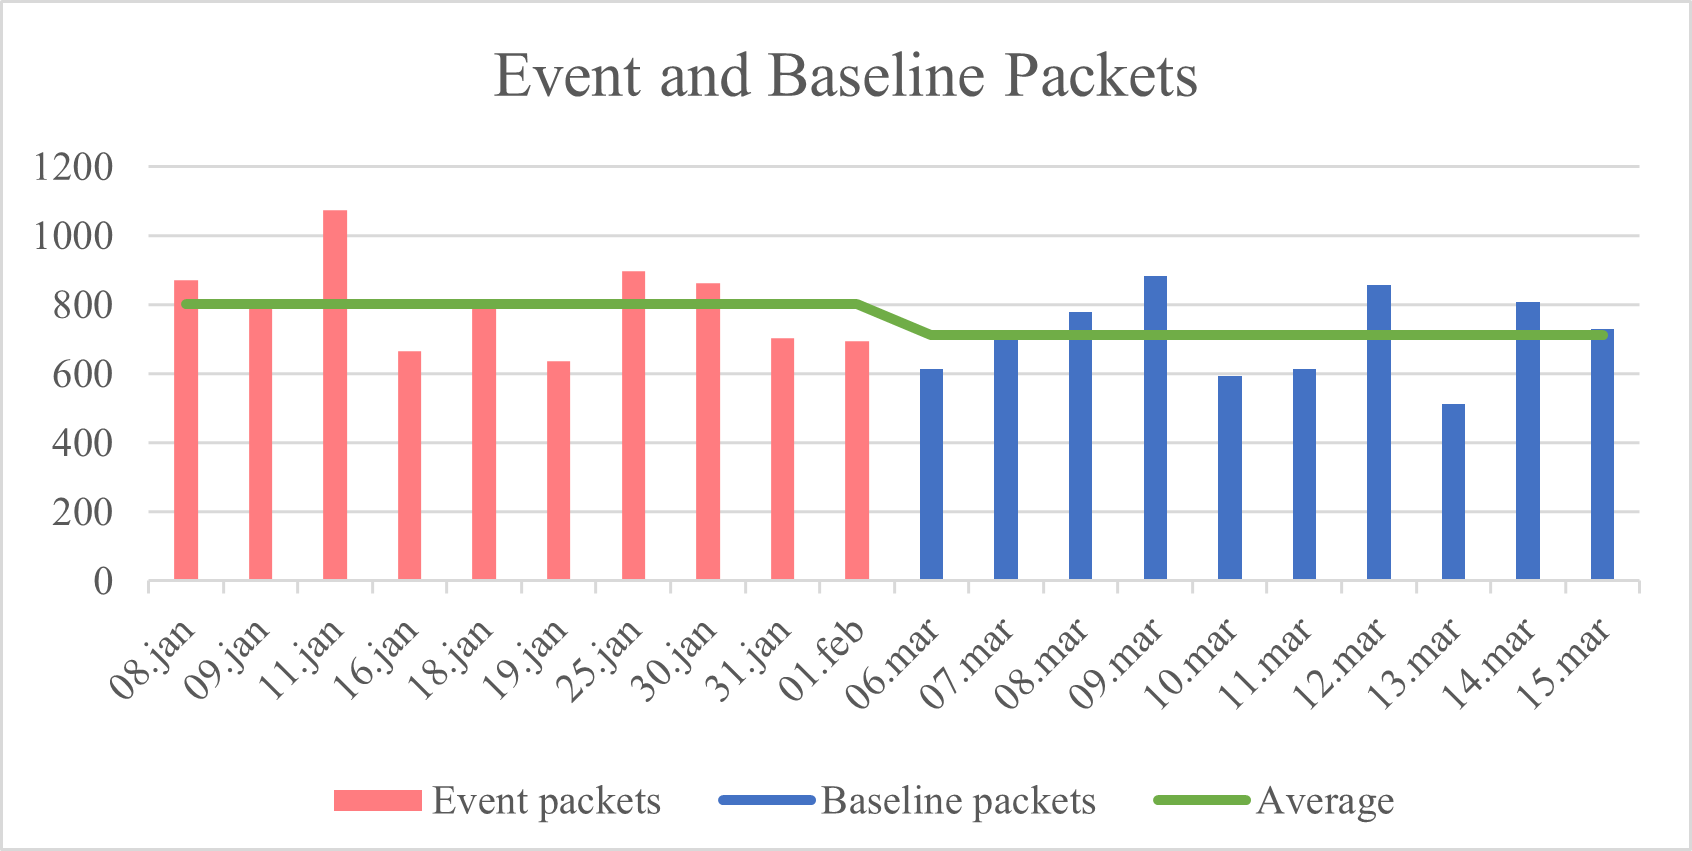
\includegraphics[width=1\hsize]{figures/Netatmo_Shower_Calculations_Packets.png} 
    \end{subfigure}
    \begin{subfigure}{0.49\textwidth}
        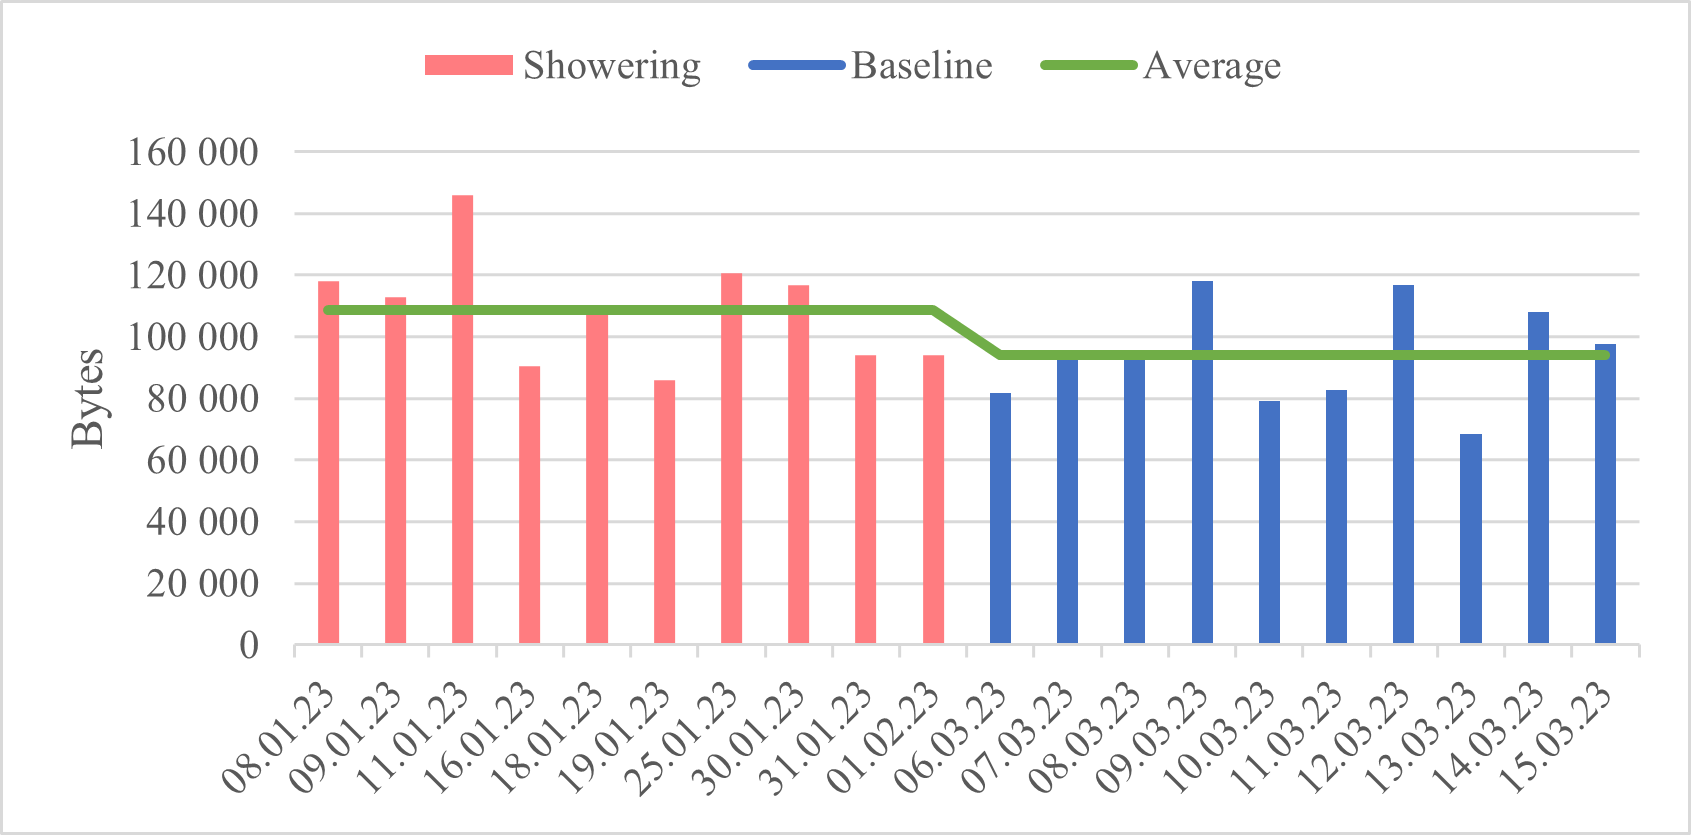
\includegraphics[width=1\hsize]{figures/Netatmo_Shower_Calculations_Bytes.png} 
    \end{subfigure}
    \caption{Graphical representation of packets and bytes with average values from Table \ref{tab:NetatmoShowerCalculations}}
    \label{fig:NetatmoShowerCalculations}
\end{figure}

\begin{figure}[H]
    \begin{subfigure}[b]{0.47\textwidth}
        \centering
        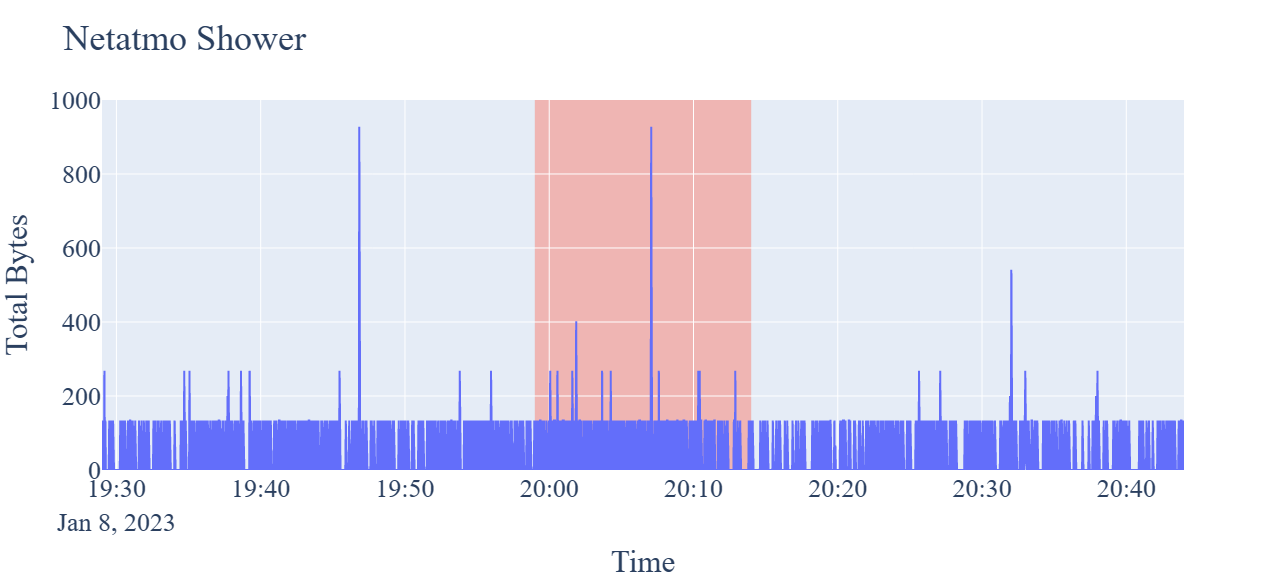
\includegraphics[width=1.2\hsize]{figures/Netatmo_Shower_Bytes_08.01.png}
    \end{subfigure}
    \begin{subfigure}[b]{0.47\textwidth}
        \centering
        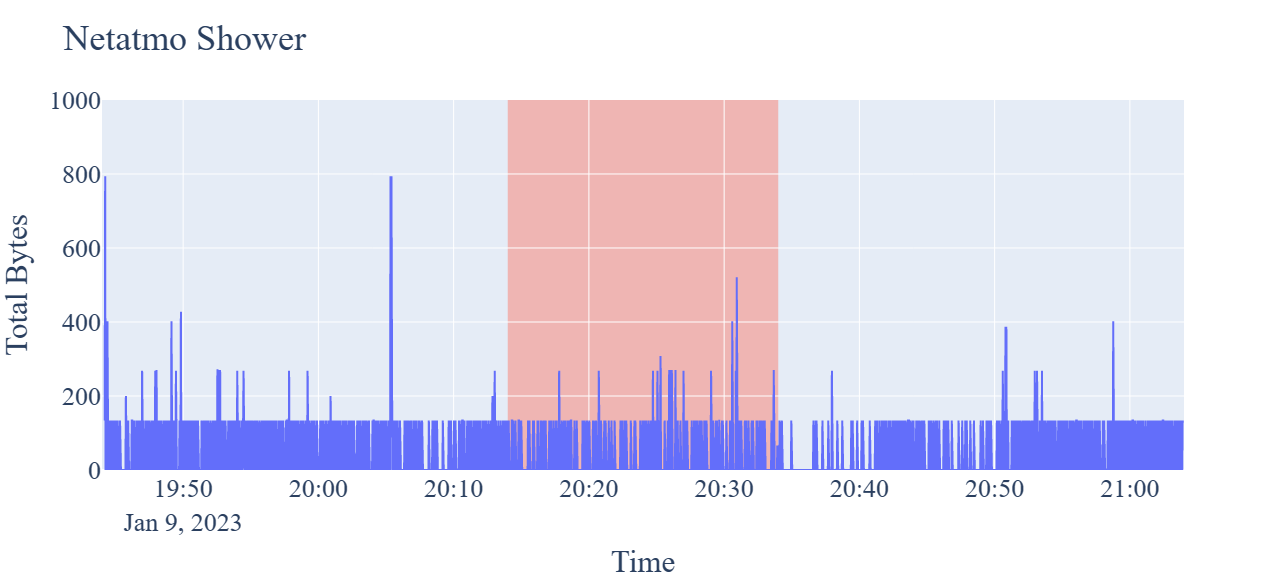
\includegraphics[width=1.2\hsize]{figures/Netatmo_Shower_Bytes_09.01.png}
    \end{subfigure}
    \begin{subfigure}[b]{0.47\textwidth}
        \centering
        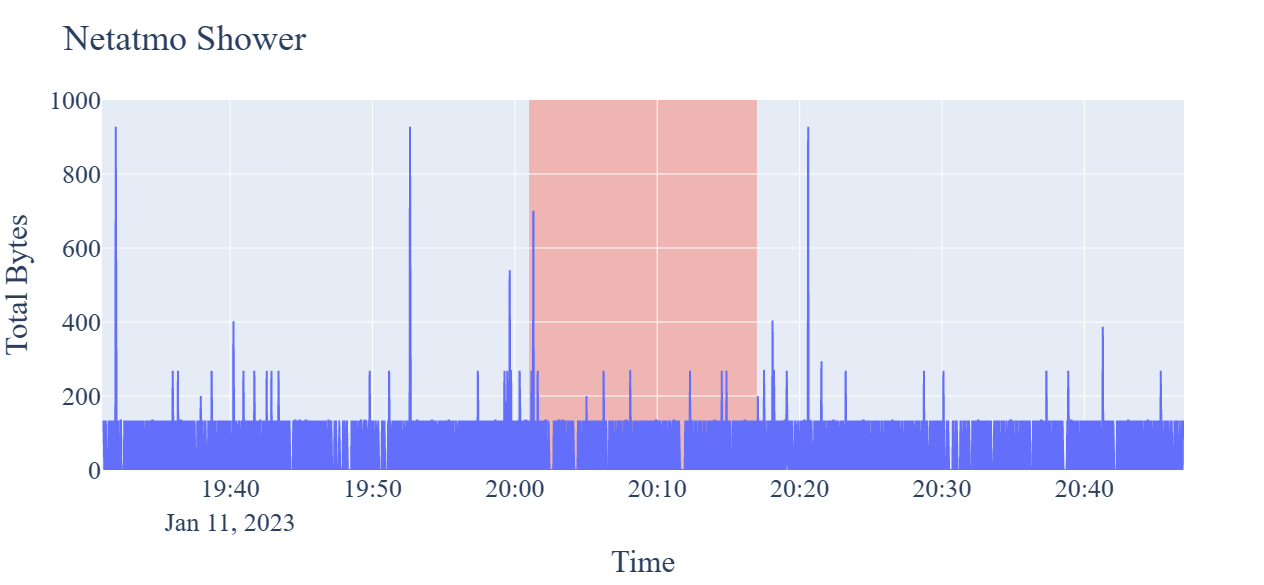
\includegraphics[width=1.2\hsize]{figures/Netatmo_Shower_Bytes_11.01.png}
    \end{subfigure}
    \begin{subfigure}[b]{0.47\textwidth}
        \centering
        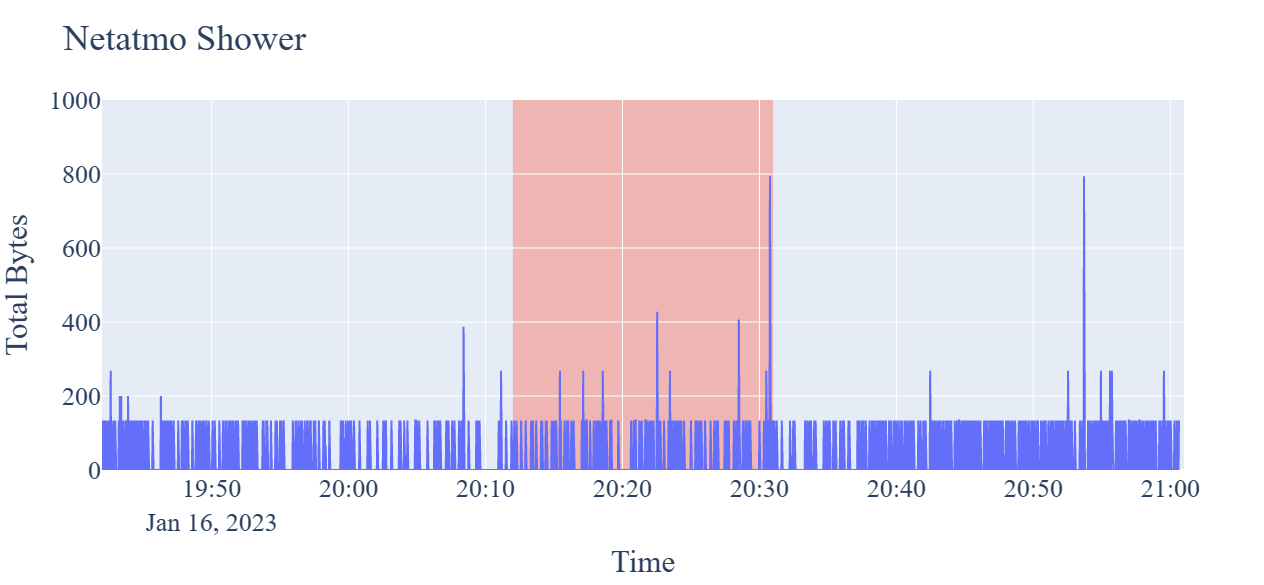
\includegraphics[width=1.2\hsize]{figures/Netatmo_Shower_Bytes_16.01.png}
    \end{subfigure}
    \begin{subfigure}[b]{0.47\textwidth}
        \centering
        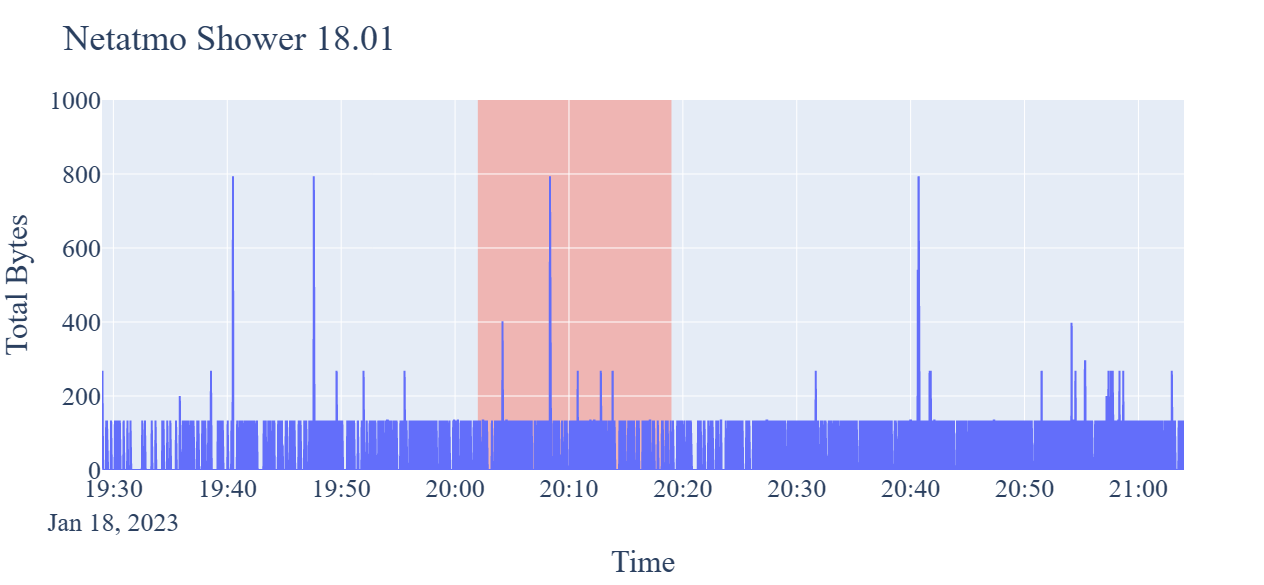
\includegraphics[width=1.2\hsize]{figures/Netatmo_Shower_Bytes_18.01.png}
    \end{subfigure}
    \begin{subfigure}[b]{0.47\textwidth}
        \centering
        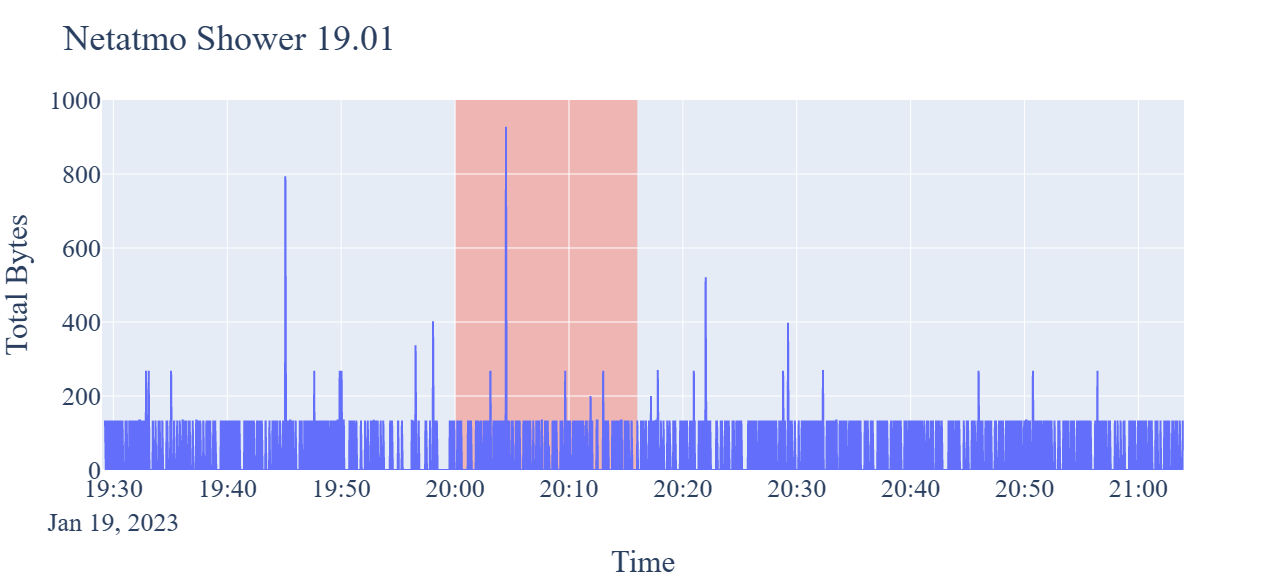
\includegraphics[width=1.2\hsize]{figures/Netatmo_Shower_Bytes_19.01.png}
    \end{subfigure}
    \begin{subfigure}[b]{0.47\textwidth}
        \centering
        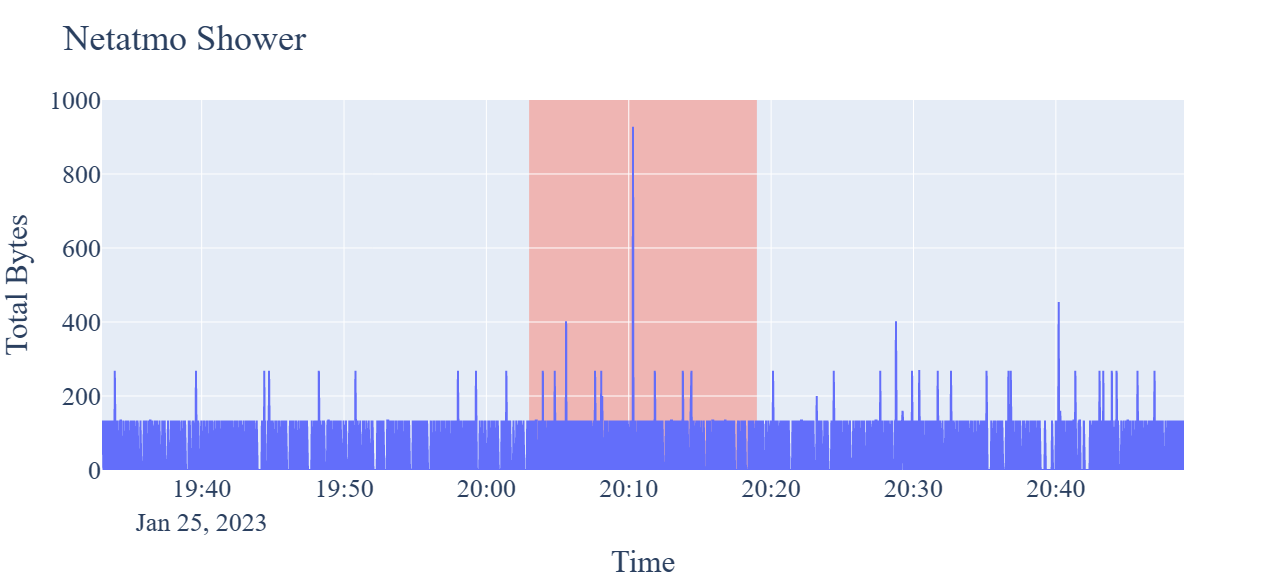
\includegraphics[width=1.2\hsize]{figures/Netatmo_Shower_Bytes_25.01.png}
    \end{subfigure}
    \begin{subfigure}[b]{0.47\textwidth}
        \centering
        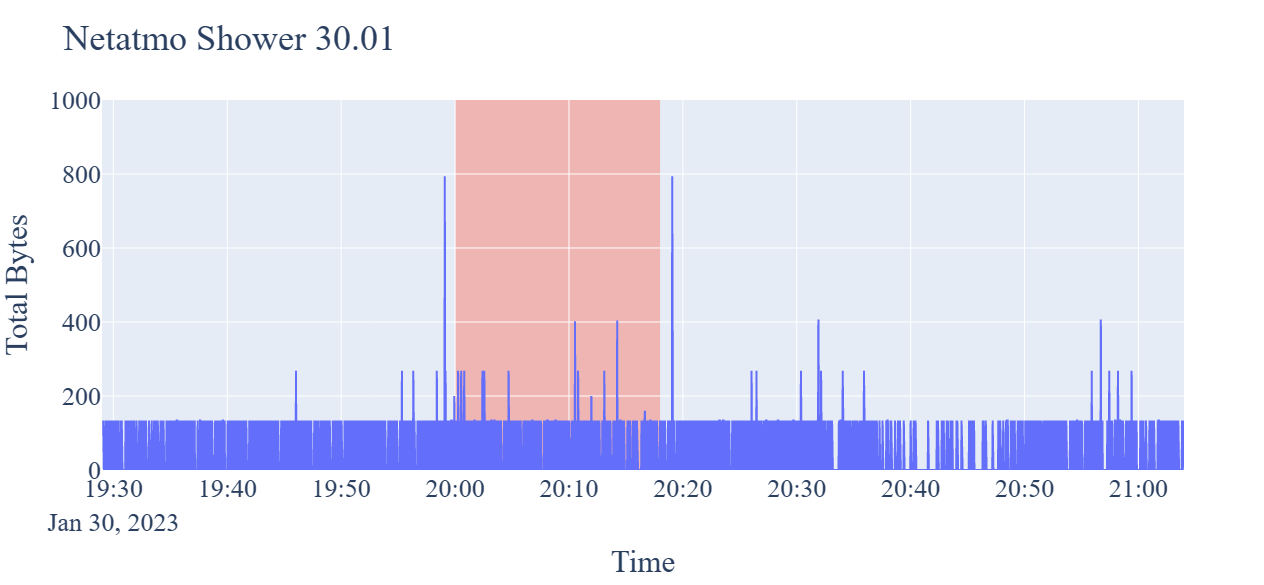
\includegraphics[width=1.2\hsize]{figures/Netatmo_Shower_Bytes_30.01.png}
    \end{subfigure}
    \begin{subfigure}[b]{0.47\textwidth}
        \centering
        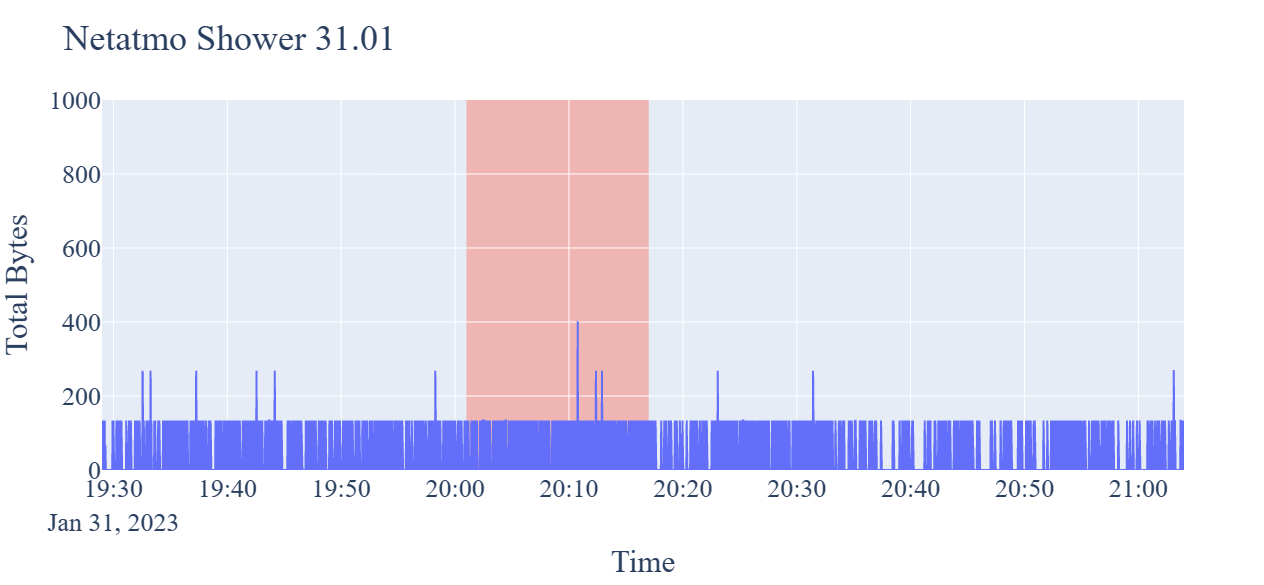
\includegraphics[width=1.2\hsize]{figures/Netatmo_Shower_Bytes_31.01.png}
    \end{subfigure}
    \hspace{0.6cm}
    \begin{subfigure}[b]{0.47\textwidth}
        \centering
        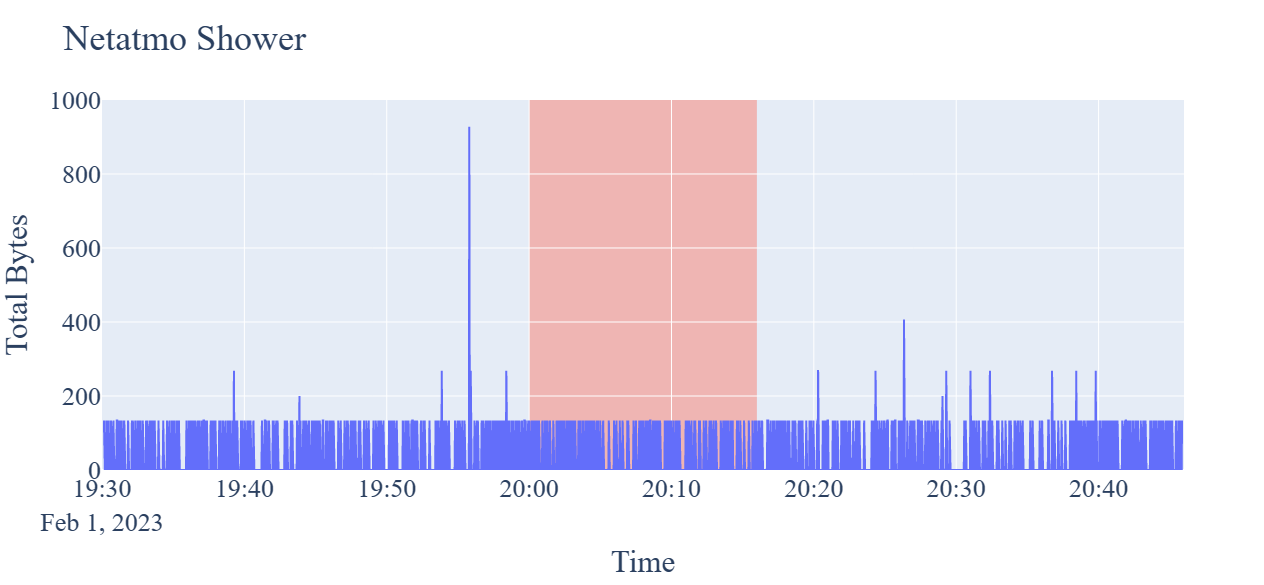
\includegraphics[width=1.2\hsize]{figures/Netatmo_Shower_Bytes_01.02.png}
    \end{subfigure}
    \caption{Netatmo Shower Events - Bytes}
    \label{fig:NetatmoShowerBytes}
\end{figure}

\begin{figure}[H]
    \begin{subfigure}[b]{0.47\textwidth}
        \centering
        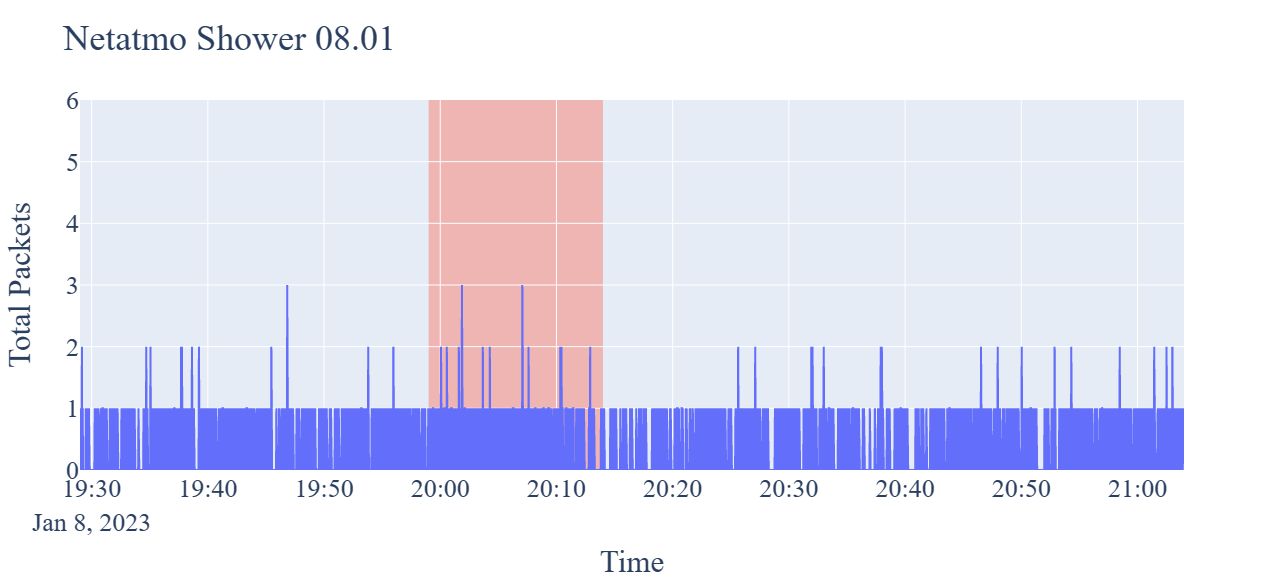
\includegraphics[width=1.2\hsize]{figures/Netatmo_Shower_Packets_08.01.png}
    \end{subfigure}
    \begin{subfigure}[b]{0.47\textwidth}
        \centering
        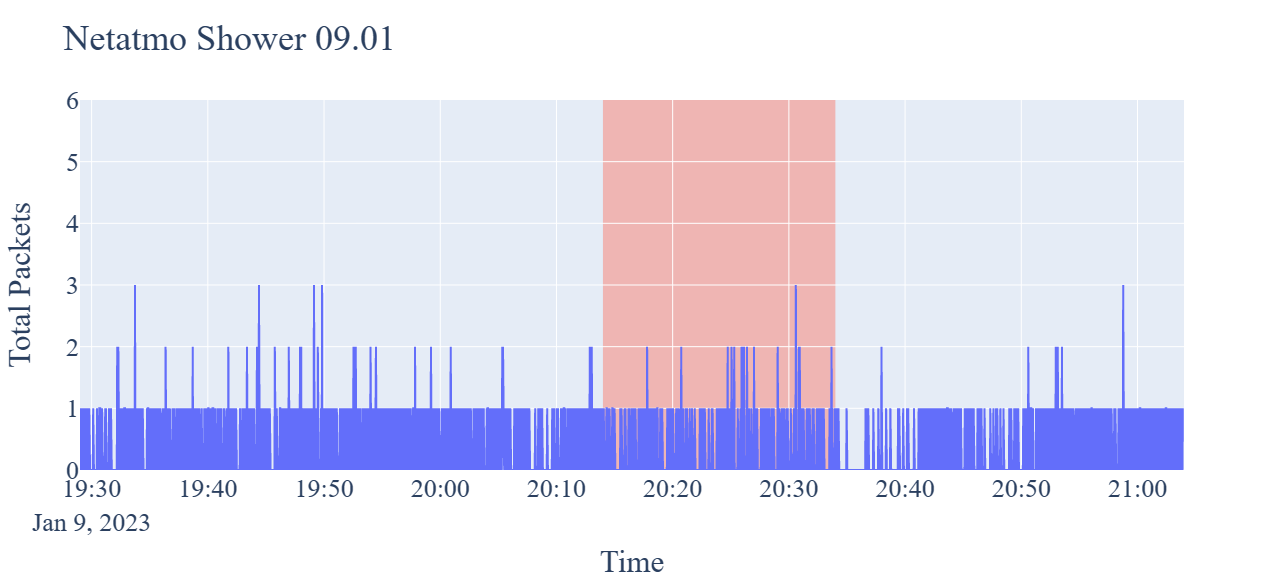
\includegraphics[width=1.2\hsize]{figures/Netatmo_Shower_Packets_09.01.png}
    \end{subfigure}
    \begin{subfigure}[b]{0.47\textwidth}
        \centering
        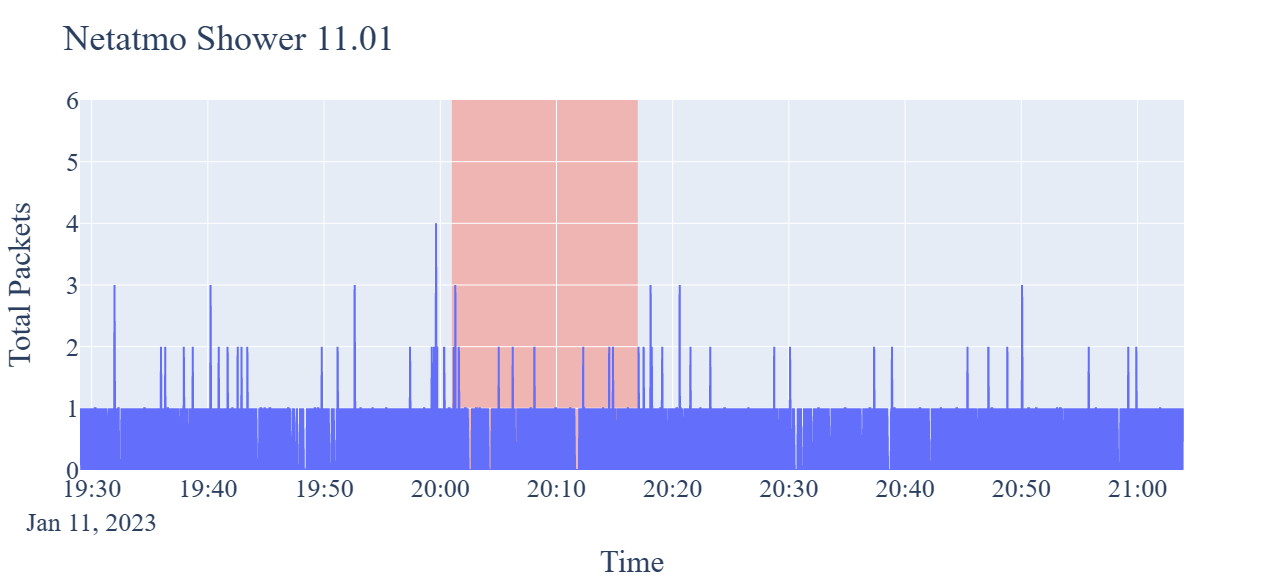
\includegraphics[width=1.2\hsize]{figures/Netatmo_Shower_Packets_11.01.png}
    \end{subfigure}
    \begin{subfigure}[b]{0.47\textwidth}
        \centering
        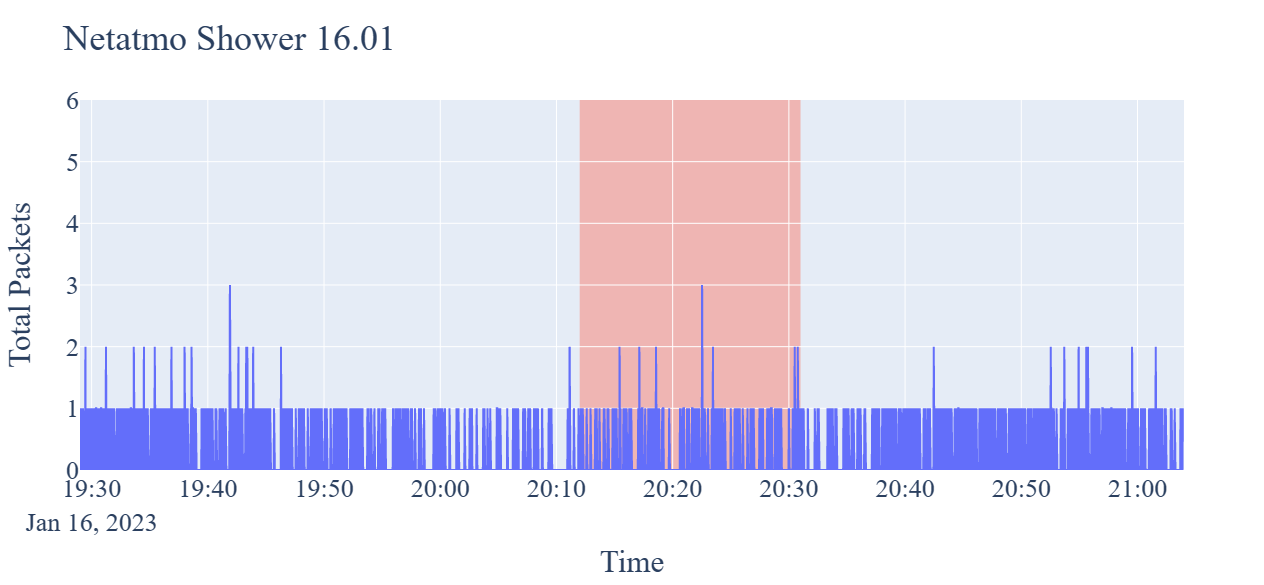
\includegraphics[width=1.2\hsize]{figures/Netatmo_Shower_Packets_16.01.png}
    \end{subfigure}
    \begin{subfigure}[b]{0.47\textwidth}
        \centering
        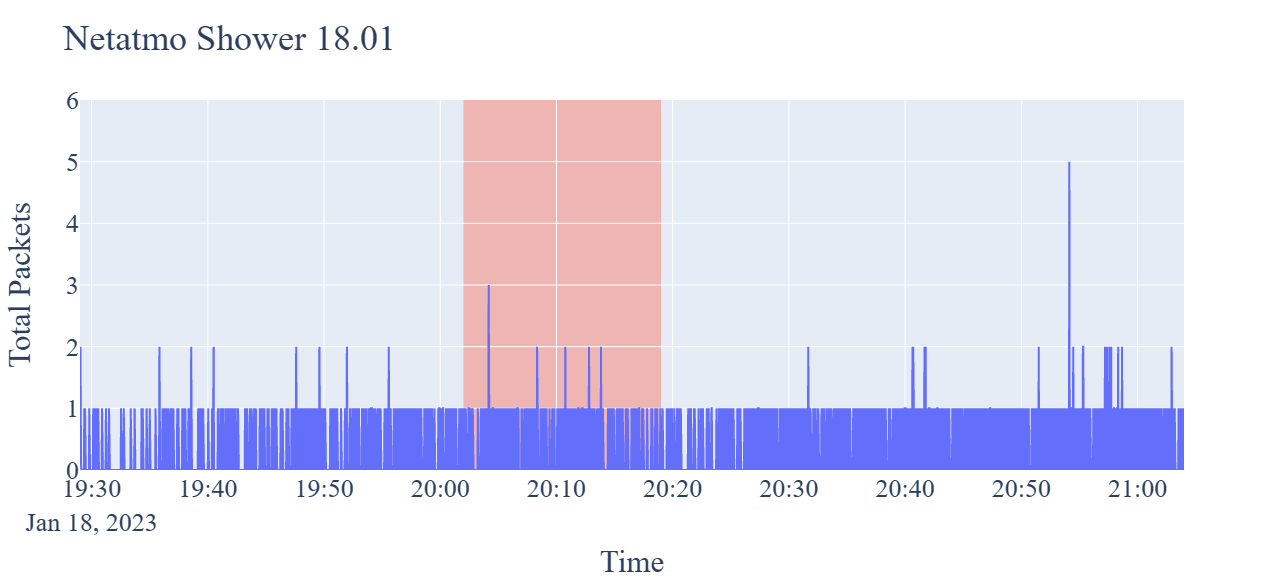
\includegraphics[width=1.2\hsize]{figures/Netatmo_Shower_Packets_18.01.png}
    \end{subfigure}
    \begin{subfigure}[b]{0.47\textwidth}
        \centering
        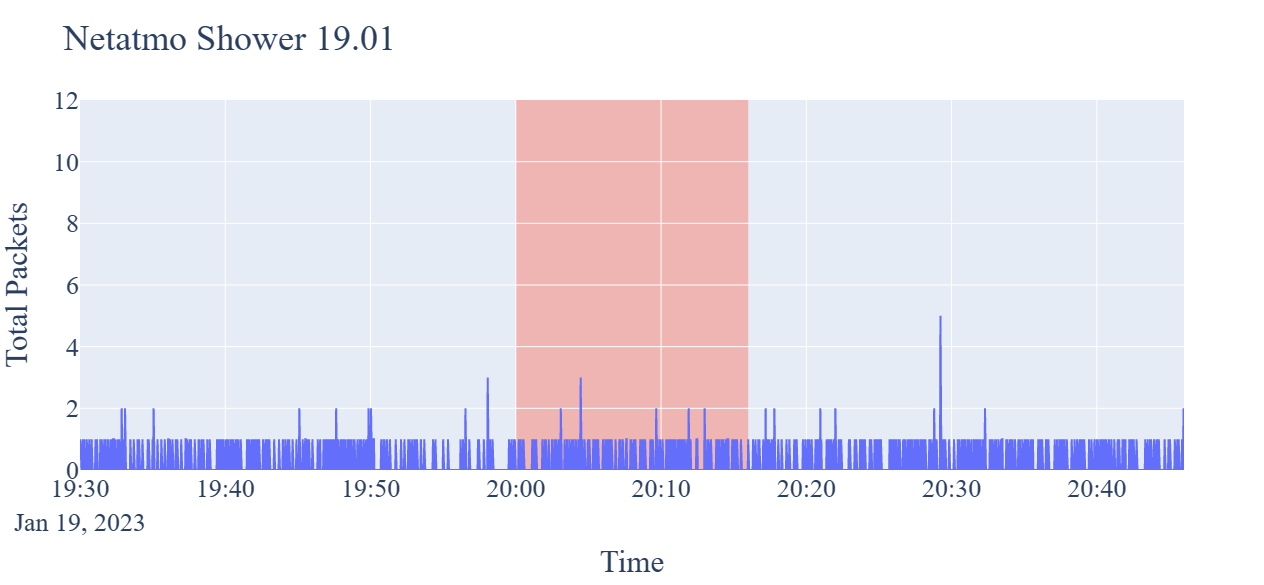
\includegraphics[width=1.2\hsize]{figures/Netatmo_Shower_Packets_19.01.png}
    \end{subfigure}
    \begin{subfigure}[b]{0.47\textwidth}
        \centering
        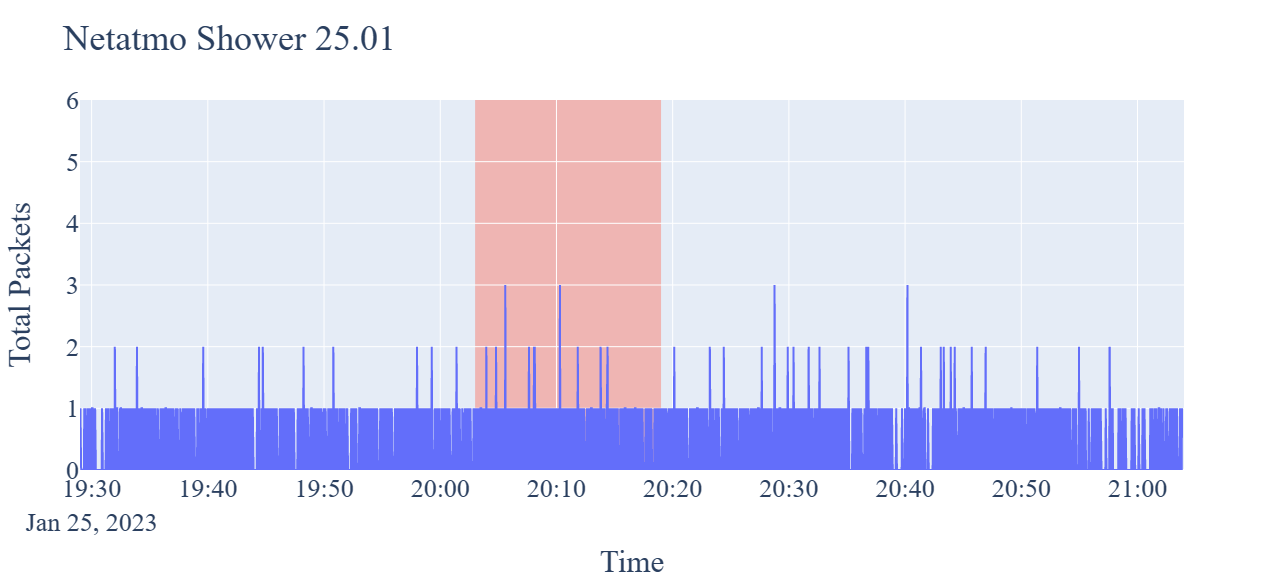
\includegraphics[width=1.2\hsize]{figures/Netatmo_Shower_Packets_25.01.png}
    \end{subfigure}
    \begin{subfigure}[b]{0.47\textwidth}
        \centering
        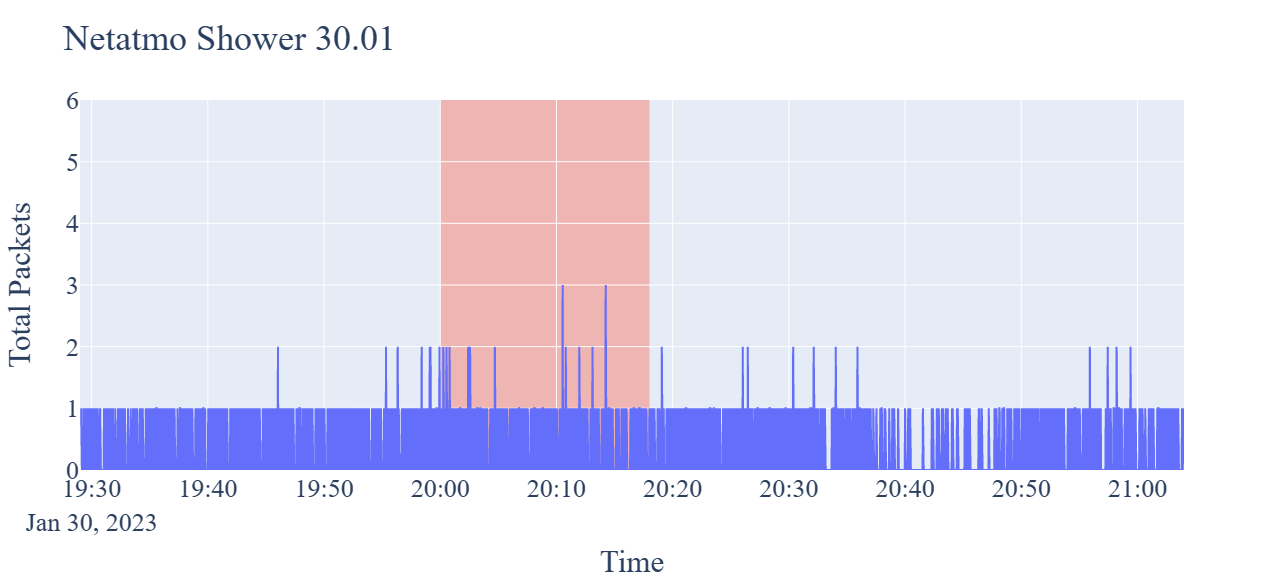
\includegraphics[width=1.2\hsize]{figures/Netatmo_Shower_Packets_30.01.png}
    \end{subfigure}
    \begin{subfigure}[b]{0.47\textwidth}
        \centering
        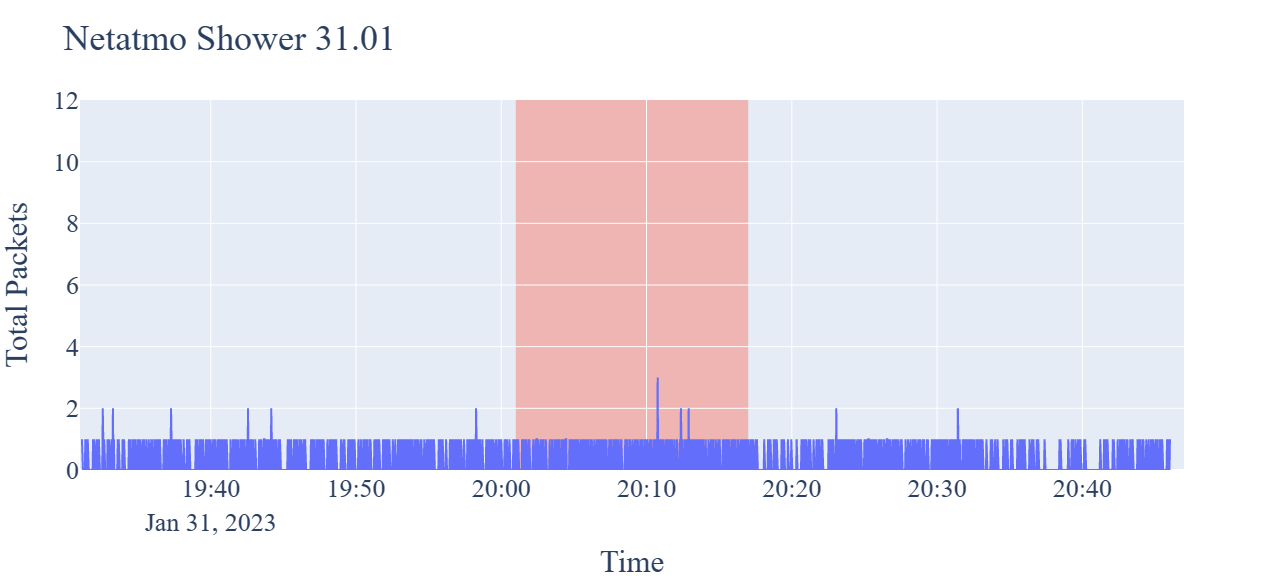
\includegraphics[width=1.2\hsize]{figures/Netatmo_Shower_Packets_31.01.png}
    \end{subfigure}
    \hspace{0.6cm}
    \begin{subfigure}[b]{0.47\textwidth}
        \centering
        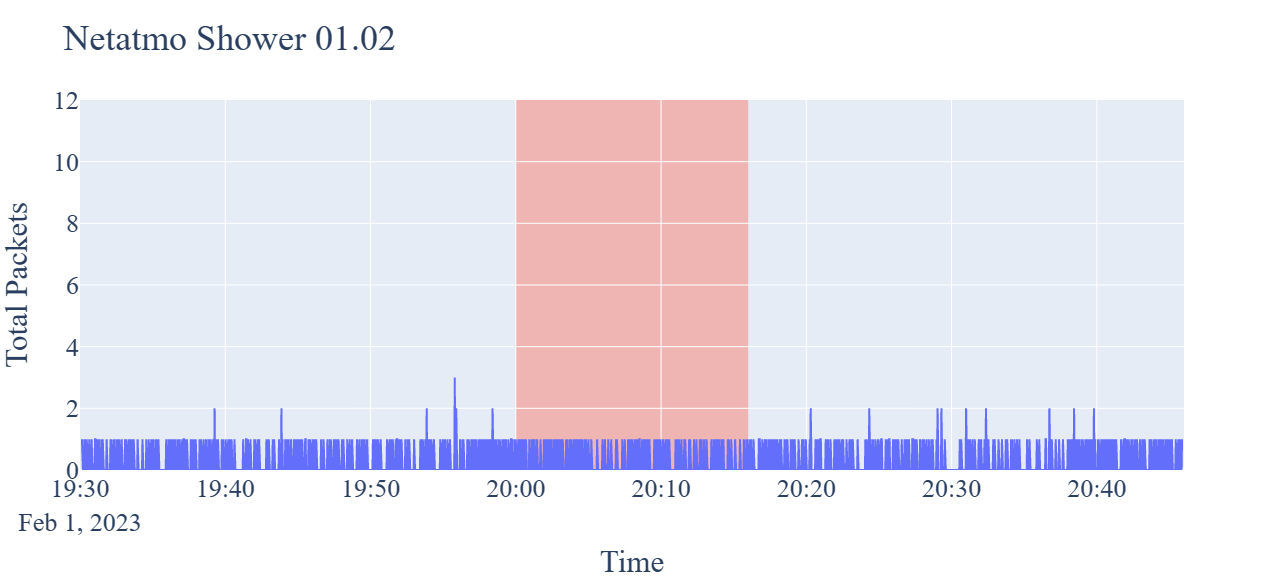
\includegraphics[width=1.2\hsize]{figures/Netatmo_Shower_Packets_01.02.png}
    \end{subfigure}
    \caption{Netatmo Shower Events - Packets}
    \label{fig:NetatmoShowerPackets}
\end{figure}

\begin{figure}[H] 
    \begin{subfigure}[b]{0.47\textwidth}
        \centering
        \tcbincludegraphics[size=fbox,width=1.1\hsize,colframe=red]{figures/Netatmo_Shower_Packets_08.01.png}
    \end{subfigure}
    \begin{subfigure}[b]{0.47\textwidth}
        \centering
        \tcbincludegraphics[size=fbox,width=1.1\hsize, colframe=blue]{figures/Netatmo_Shower_Baseline_Packets_06.03.png}
    \end{subfigure}
    \begin{subfigure}[b]{0.47\textwidth}
        \centering
        \tcbincludegraphics[size=fbox,width=1.1\hsize,colframe=red]{figures/Netatmo_Shower_Packets_09.01.png}
    \end{subfigure}
    \begin{subfigure}[b]{0.47\textwidth}
        \centering
        \tcbincludegraphics[size=fbox,width=1.1\hsize,colframe=blue]{figures/Netatmo_Shower_Baseline_Packets_07.03.png}
    \end{subfigure}
    \begin{subfigure}[b]{0.47\textwidth}
        \centering
        \tcbincludegraphics[size=fbox,width=1.1\hsize,colframe=red]{figures/Netatmo_Shower_Packets_11.01.png}
    \end{subfigure}
    \begin{subfigure}[b]{0.47\textwidth}
        \centering
        \tcbincludegraphics[size=fbox,width=1.1\hsize,colframe=blue]{figures/Netatmo_Shower_Baseline_Packets_08.03.png}
    \end{subfigure}
    \begin{subfigure}[b]{0.47\textwidth}
        \centering
        \tcbincludegraphics[size=fbox,width=1.1\hsize,colframe=red]{figures/Netatmo_Shower_Packets_16.01.png}
    \end{subfigure}
    \begin{subfigure}[b]{0.47\textwidth}
        \centering
        \tcbincludegraphics[size=fbox,width=1.1\hsize,colframe=blue]{figures/Netatmo_Shower_Baseline_Packets_09.03.png}
    \end{subfigure}
    \begin{subfigure}[b]{0.47\textwidth}
        \centering
        \tcbincludegraphics[size=fbox,width=1.1\hsize,colframe=red]{figures/Netatmo_Shower_Packets_18.01.png}
    \end{subfigure}
    \begin{subfigure}[b]{0.47\textwidth}
        \centering
        \tcbincludegraphics[size=fbox,width=1.1\hsize,colframe=blue]{figures/Netatmo_Shower_Baseline_Packets_10.03.png}
    \end{subfigure}
        \begin{subfigure}[b]{0.47\textwidth}
        \centering
        \tcbincludegraphics[size=fbox,width=1.1\hsize,colframe=red]{figures/Netatmo_Shower_Packets_19.01.png}
    \end{subfigure}
    \begin{subfigure}[b]{0.47\textwidth}
        \centering
        \tcbincludegraphics[size=fbox,width=1.1\hsize,colframe=blue]{figures/Netatmo_Shower_Baseline_Packets_11.03.png}
    \end{subfigure}
    \begin{subfigure}[b]{0.47\textwidth}
        \centering
        \tcbincludegraphics[size=fbox,width=1.1\hsize,colframe=red]{figures/Netatmo_Shower_Packets_25.01.png}
    \end{subfigure}
    \hspace{0.6cm}
    \begin{subfigure}[b]{0.47\textwidth}
        \centering
        \tcbincludegraphics[size=fbox,width=1.1\hsize,colframe=blue]{figures/Netatmo_Shower_Baseline_Packets_12.03.png}
    \end{subfigure}
    \caption{Comparing Events and Baseline Packets for Shower - Netatmo 1}
    \label{fig:NetatmoShowerComparingPackets1}
\end{figure}

\begin{figure}
   \begin{subfigure}[b]{0.47\textwidth}
        \centering
        \tcbincludegraphics[size=fbox,width=1.1\hsize,colframe=red]{figures/Netatmo_Shower_Packets_30.01.png}
    \end{subfigure}
    \begin{subfigure}[b]{0.47\textwidth}
        \centering
        \tcbincludegraphics[size=fbox,width=1.1\hsize,colframe=blue]{figures/Netatmo_Shower_Baseline_Packets_13.03.png}
    \end{subfigure}
        \begin{subfigure}[b]{0.47\textwidth}
        \centering
        \tcbincludegraphics[size=fbox,width=1.1\hsize,colframe=red]{figures/Netatmo_Shower_Packets_31.01.png}
    \end{subfigure}
    \begin{subfigure}[b]{0.47\textwidth}
        \centering
        \tcbincludegraphics[size=fbox,width=1.1\hsize,colframe=blue]{figures/Netatmo_Shower_Baseline_Packets_14.03.png}
    \end{subfigure}
    \begin{subfigure}[b]{0.47\textwidth}
        \centering
        \tcbincludegraphics[size=fbox,width=1.1\hsize,colframe=red]{figures/Netatmo_Shower_Packets_01.02.png}
    \end{subfigure}
    \hspace{0.6cm}
    \begin{subfigure}[b]{0.47\textwidth}
    \centering
        \tcbincludegraphics[size=fbox,width=1.1\hsize,colframe=blue]{figures/Netatmo_Shower_Baseline_Packets_15.03.png}
        \end{subfigure}
    \caption{Comparing Events and Baseline Packets for Shower - Netatmo 2}
    \label{fig:NetatmoShowerComparingPackets2}
\end{figure}

\begin{figure}[H]
    \begin{subfigure}[b]{0.47\textwidth}
        \centering
        \tcbincludegraphics[size=fbox,width=1.1\hsize,colframe=red]{figures/Netatmo_Shower_Bytes_08.01.png}
    \end{subfigure}
    \begin{subfigure}[b]{0.47\textwidth}
        \centering
        \tcbincludegraphics[size=fbox,width=1.1\hsize,colframe=blue]{figures/Netatmo_Shower_Baseline_Bytes_06.03.png}
    \end{subfigure}
    \begin{subfigure}[b]{0.47\textwidth}
        \centering
        \tcbincludegraphics[size=fbox,width=1.1\hsize,colframe=red]{figures/Netatmo_Shower_Bytes_09.01.png}
    \end{subfigure}
    \begin{subfigure}[b]{0.47\textwidth}
        \centering
        \tcbincludegraphics[size=fbox,width=1.1\hsize,colframe=blue]{figures/Netatmo_Shower_Baseline_Bytes_07.03.png}
    \end{subfigure}
    \begin{subfigure}[b]{0.47\textwidth}
        \centering
        \tcbincludegraphics[size=fbox,width=1.1\hsize,colframe=red]{figures/Netatmo_Shower_Bytes_11.01.png}
    \end{subfigure}
    \hspace{0.6cm}
    \begin{subfigure}[b]{0.47\textwidth}
        \centering
        \tcbincludegraphics[size=fbox,width=1.1\hsize,colframe=blue]{figures/Netatmo_Shower_Baseline_Bytes_08.03.png}
    \end{subfigure}
    \caption{Comparing Events and Baseline Bytes for Shower - Netatmo 1}
    \label{fig:NetatmoShowerComparingBytes 1}
\end{figure}

\begin{figure}[H]
 \begin{subfigure}[b]{0.47\textwidth}
        \centering
        \tcbincludegraphics[size=fbox,width=1.1\hsize,colframe=red]{figures/Netatmo_Shower_Bytes_16.01.png}
    \end{subfigure}
    \begin{subfigure}[b]{0.47\textwidth}
        \centering
        \tcbincludegraphics[size=fbox,width=1.1\hsize,colframe=blue]{figures/Netatmo_Shower_Baseline_Bytes_09.03.png}
    \end{subfigure}
    \begin{subfigure}[b]{0.47\textwidth}
        \centering
        \tcbincludegraphics[size=fbox,width=1.1\hsize,colframe=red]{figures/Netatmo_Shower_Bytes_18.01.png}
    \end{subfigure}
    \begin{subfigure}[b]{0.47\textwidth}
        \centering
        \tcbincludegraphics[size=fbox,width=1.1\hsize,colframe=blue]{figures/Netatmo_Shower_Baseline_Bytes_10.03.png}
    \end{subfigure}
        \begin{subfigure}[b]{0.47\textwidth}
        \centering
        \tcbincludegraphics[size=fbox,width=1.1\hsize,colframe=red]{figures/Netatmo_Shower_Bytes_19.01.png}
    \end{subfigure}
    \begin{subfigure}[b]{0.47\textwidth}
        \centering
        \tcbincludegraphics[size=fbox,width=1.1\hsize,colframe=blue]{figures/Netatmo_Shower_Baseline_Bytes_11.03.png}
    \end{subfigure}
    \begin{subfigure}[b]{0.47\textwidth}
        \centering
        \tcbincludegraphics[size=fbox,width=1.1\hsize,colframe=red]{figures/Netatmo_Shower_Bytes_25.01.png}
    \end{subfigure}
    \begin{subfigure}[b]{0.47\textwidth}
        \centering
        \tcbincludegraphics[size=fbox,width=1.1\hsize,colframe=blue]{figures/Netatmo_Shower_Baseline_Bytes_12.03.png}
    \end{subfigure}
        \begin{subfigure}[b]{0.47\textwidth}
        \centering
        \tcbincludegraphics[size=fbox,width=1.1\hsize,colframe=red]{figures/Netatmo_Shower_Bytes_30.01.png}
    \end{subfigure}
    \begin{subfigure}[b]{0.47\textwidth}
        \centering
        \tcbincludegraphics[size=fbox,width=1.1\hsize,colframe=blue]{figures/Netatmo_Shower_Baseline_Bytes_13.03.png}
    \end{subfigure}
        \begin{subfigure}[b]{0.47\textwidth}
        \centering
        \tcbincludegraphics[size=fbox,width=1.1\hsize,colframe=red]{figures/Netatmo_Shower_Bytes_31.01.png}
    \end{subfigure}
    \begin{subfigure}[b]{0.47\textwidth}
        \centering
        \tcbincludegraphics[size=fbox,width=1.1\hsize,colframe=blue]{figures/Netatmo_Shower_Baseline_Bytes_14.03.png}
    \end{subfigure}
        \begin{subfigure}[b]{0.47\textwidth}
        \centering
        \tcbincludegraphics[size=fbox,width=1.1\hsize,colframe=red]{figures/Netatmo_Shower_Bytes_01.02.png}
    \end{subfigure}
    \hspace{0.6cm}
    \begin{subfigure}[b]{0.47\textwidth}
        \centering
        \tcbincludegraphics[size=fbox,width=1.1\hsize,colframe=blue]{figures/Netatmo_Shower_Baseline_Bytes_15.03.png}
    \end{subfigure}
    \caption{Comparing Events and Baseline Bytes for Shower - Netatmo 2}
    \label{fig:NetatmoShowerComparingBytes2}
\end{figure}

\begin{table}[H]
    \centering
    \caption{Netatmo Baseline Shower Calculations}
    \begin{tabular}{|l|l|l|l|}
    \hline
        \textbf{Baseline} & \textbf{Packets} & \textbf{Bytes} & \textbf{Biggest   packet} \\ \hline
        06.mar            & 473              & 63,182          & 407 bytes                \\ \hline
        07.mar            & 572              & 76,172          & 136 bytes                \\ \hline
        08.mar            & 597              & 79,966          & 160 bytes                \\ \hline
        09.mar            & 740              & 98,888          & 134 bytes                \\ \hline
        10.mar            & 514              & 68,806          & 136 bytes                \\ \hline
        11.mar            & 510              & 68,594          & 407 bytes                \\ \hline
        12.mar            & 741              & 101,295         & 407 bytes                \\ \hline
        13.mar            & 422              & 56,142          & 136 bytes                \\ \hline
        14.mar            & 697              & 93,246          & 407 bytes                \\ \hline
        15.mar            & 600              & 80,128          & 134 bytes                \\ \hline
\textbf{Average}  & \textbf{587}     & \textbf{78,642} & \textbf{246 bytes}               \\ \hline
\textbf{Std dev}  & \textbf{111}     & \textbf{15,237} & \textbf{138 bytes}               \\ \hline
    \end{tabular}
    \label{tab:NetatmoBaselineShowerCalculations}
\end{table}

\begin{table}[H]
    \centering
    \caption{Comparing Shower and Baseline Calculations for Netatmo}
    \begin{tabular}{c|l|l|l|l|}
        \cline{2-5}
        \multicolumn{1}{l|}{} & \textbf{Type} & \textbf{Packets} & \textbf{Bytes} & \textbf{Biggest packet} \\ \hline
        \multicolumn{1}{|c|}{\multirow{2}{*}{\textbf{Average}}}  & Event & 674 & 91,663 & 390 bytes \\ \cline{2-5} 
        \multicolumn{1}{|c|}{}  & Baseline  & 587 & 78,642 & 246 bytes \\ \hline
        \multicolumn{1}{|c|}{\multirow{2}{*}{\textbf{Standard deviation}}} & Event & 170 & 23,072 & 70 bytes \\ \cline{2-5} 
        \multicolumn{1}{|c|}{} & Baseline & 111 & 15,237 & 138 bytes\\ \hline          
    \end{tabular}
    \label{tab:NetatmoComparingBaselineAndShowerCalculations}
\end{table}

\begin{figure}[H]
    \centering
    \begin{subfigure}{0.49\textwidth}
        \centering
        \includegraphics[width=1\hsize]{figures/Netatmo_Comparing_Shower_Calculations_Bytes.png} 
    \end{subfigure}
    \begin{subfigure}{0.49\textwidth}
        \centering
        \includegraphics[width=1\hsize]{figures/Netatmo_Comparing_Shower_Calculations_Packets.png} 
    \end{subfigure}
    \caption{Comparing Shower Calculations for Netatmo}
    \label{fig:NetatmoComparingShowerCalculations}
\end{figure}


\subsection{Mill Sense}
\subsection{Nedis}

\newpage
\section{Test Case 3: Window Open}
This chapter presents the results and analysis conducted on Test Case 3: Window Open. 
\subsection{General}
\begin{table}[!hbtp]
    \centering
    \caption{Date and time for Test Case 3: Window Open events}
    \begin{adjustbox}{width=1\textwidth} 
            \begin{tabular}{l|l|l|l|l|l|l|l|l|l|l|l|l|l|l|l|}
                \cline{2-16}
                & 08.01 & 09.01 & 10.01 & 11.01 & 12.01 & 16.01 & 18.01 & 19.01 & 23.01 & 24.01 & 25.01 & 30.01 & 31.01 & 01.02 & 02.02 \\ \hline
                \multicolumn{1}{|l|}{Started event}  & 23:00 & 23:00 & 23:00 & 22:50 & 23:00 & 23:10 & 23:15 & 23:02 & 22:59 & 22:59 & 22:59 & 23:00 & 22:59 & 22:59 & 22:59 \\ \hline
                \multicolumn{1}{|l|}{Finished event} & 07:00 & 07:00 & 07:00 & 07:00 & 07:00 & 06:56 & 07:09 & 06:59 & 06:55 & 06:57 & 06:55 & 06:56 & 07:00 & 06:59 & 06:59 \\ \hline
            \end{tabular}
    \end{adjustbox}
    \label{tab:WindowDates}
\end{table}
\subsection{Netatmo Home Coach}
\subsection{Mill Sense}
\subsection{Nedis}

\newpage
\newpage
\section{Test Case 4: Weekends}
This chapter presents the results and analysis conducted on Test Case 4: Weekends. 
\subsection{General}
Test Case 4: Weekends are tested over the course of 14 different weekends. 7 weekends when the environment was occupied and 7 when the environment were not occupied. The different dates are described in table \ref{tab:WeekendDates}. 
\begin{table}[H]
    \centering
    \caption{Dates for Test Case 4: Weekends}
    \begin{adjustbox}{width=0.5\textwidth} 
        \begin{tabular}{l|l|}
            \cline{2-2} & \textbf{Dates}\\ \hline
            \multicolumn{1}{|l|}{\textbf{Occupied (Home)}} & \begin{tabular}[c]{@{}l@{}}13.01.2023-15.01.2023\\ 27.01.2023-29.01.2023\\ 03.02.2023-05.02.2023\\ 17.02.2023-19.02.2023\\ 10.03.2023-12.03.2023\\ 28.03.2023-30.03.2023\\ 31.03.2023-01.04.2023\end{tabular} \\ \hline
            \multicolumn{1}{|l|}{\textbf{Not occupied (Gone)}} & \begin{tabular}[c]{@{}l@{}}23.12.2022-25.12.2022\\ 30.12.2022-01.01.2023\\ 20.01.2023-22.01.2023\\ 10.02.2023-12.02.2023\\ 24.02.2023-26.02.2023\\ 03.03.2023-05.03.2023\\ 17.03.2023-19.03.2023\end{tabular} \\ \hline
        \end{tabular}
    \end{adjustbox}
    \label{tab:WeekendDates}
\end{table}

The times for home and gone were from 16:00 at Friday to 22:00 at Sunday, which means that when a weekend gone were tested, the home was empty in those times. However, in a weekend were the home was occupied, it was variably occupied. Some weekends a lot of time were spent in the home and other weekends it was just occupied during evenings or daytime, but every occupied weekend were spent sleeping at night in the home. One weekend, 28.03.2023-30.03.2023, are actually Tuesday to Thursday, but are treated as Tuesday=Friday and Thursday=Sunday. 
\newpage
\subsection{Netatmo Home Coach}
For the weekend test for Netatmo, both calculations and graphs of the traffic are presented. The calculations for the weekends are listed in Table \ref{tab:NetatmoHomeWeekends} and \ref{tab:NetatmoGoneWeekends}. Table \ref{tab:NetatmoWeekends} compares the average and standard deviation for the weekends at home and gone. Graphs for packets are presented in Figure \ref{fig:NetatmoWeekendPackets} and bytes in Figure \ref{fig:NetatmoWeekendBytes}. In these two figures, the weekends when at home are framed with green and placed on the left side of the figure and the weekends when the home was not occupied are framed with orange and placed on the right side of the figure. All graphs the graphs in each figure have the same maximum value on the y-axis and have the same amount of time on the x-axis to be easily comparable. 

\begin{table}[H]
    \caption{Netatmo: Weekend Calculations for Home}
    \begin{tabular}{|l|l|l|l|l|l|}
    \hline
        \textbf{Date} & \textbf{Packets} & \textbf{Bytes}  & \textbf{Biggest src} & \textbf{Biggest dst} \\ \hline
        13.01-15.01   & 31,640           & 4,285,664       & 407 bytes            & 418 bytes            \\ \hline
        27.01-29.01   & 25,465           & 3,436,632       & 407 bytes            & 154 bytes            \\ \hline
        03.02-05.02   & 24,887           & 3,379,806       & 444 bytes            & 396 bytes            \\ \hline
        17.02-19.02   & 23,654           & 3,202,102       & 1,130 bytes          & 154 bytes            \\ \hline
        10.03-12.03   & 24,881           & 3,372,230       & 407 bytes            & 136 bytes            \\ \hline
        28.03-30.03   & 27,555           & 3,743,121       & 407 bytes            & 154 bytes            \\ \hline
        31.03-02.04   & 28,445           & 3,852,003       & 407 bytes            & 418 bytes            \\ \hline
    \end{tabular}
    \label{tab:NetatmoHomeWeekends}
\end{table}

\begin{table}[H]
    \caption{Netatmo: Weekend Calculations for Gone}
    \begin{tabular}{|l|l|l|l|l|l|}
    \hline
        \textbf{Date} & \textbf{Packets} & \textbf{Bytes} & \textbf{Biggest src} & \textbf{Biggest dst} \\ \hline
        23.12-25.12   & 22,367           & 2,987,324      & 134 bytes            & 136 bytes            \\ \hline
        30.12-01.01   & 22,553           & 3,012,868      & 134 bytes            & 136 bytes            \\ \hline
        20.01-22.01   & 24,631           & 3,288,842      & 134 bytes            & 154 bytes            \\ \hline
        10.02-12.02   & 20,320           & 2,715,486      & 134 bytes            & 136 bytes            \\ \hline
        24.02-26.02   & 21,332           & 2,849,186      & 134 bytes            & 136 bytes            \\ \hline
        03.03-05.03   & 19,023           & 2,538,937      & 134 bytes            & 136 bytes            \\ \hline
        17.03-19.03   & 23,905           & 3,191,924      & 134 bytes            & 136 bytes            \\ \hline
    \end{tabular}
    \label{tab:NetatmoGoneWeekends}
\end{table}

\begin{table}[H]
    \caption{Netatmo: Comparing Weekend Values}
    \begin{tabular}{ll|l|l|l|l|l|}
        \cline{3-7}
        &      & \textbf{Packets} & \textbf{Bytes} & \textbf{Biggest src} & \textbf{Biggest dst} \\ \hline
    \multicolumn{1}{|l|}{\multirow{2}{*}{\textbf{Avg}}} & Home & 26,647          & 3,610,223    & 516 bytes                 & 261 bytes                 \\ \cline{2-7} 
    \multicolumn{1}{|l|}{}                              & Gone & 22,019          & 2,940,652    & 134 bytes                    & 139 bytes                 \\ \hline
    \multicolumn{1}{|l|}{\multirow{2}{*}{\textbf{SD}}} & Home & 2,756            & 373,892      & 271 bytes                 & 140 bytes                 \\ \cline{2-7} 
    \multicolumn{1}{|l|}{}                             & Gone & 1,963            & 262,109      & 0 bytes                   & 7 bytes                   \\ \hline
    \end{tabular}
    \label{tab:NetatmoWeekends}
\end{table}

\begin{figure} [H]
    \begin{subfigure}[b]{0.47\textwidth}
    \centering
        \tcbincludegraphics[size=fbox,width=1.1\hsize,colframe=green]{figures/Netatmo_Weekend_Packets_13.01-15.01.png}
    \end{subfigure}
    \begin{subfigure}[b]{0.47\textwidth}
    \centering
        \tcbincludegraphics[size=fbox,width=1.1\hsize,colframe=orange]{figures/Netatmo_Weekend_Packets_23.12-25.12.png}
    \end{subfigure}
    \begin{subfigure}[b]{0.47\textwidth}
        \tcbincludegraphics[size=fbox,width=1.1\hsize,colframe=green]{figures/Netatmo_Weekend_Packets_27.01-29.01.png}
    \end{subfigure}
    \begin{subfigure}[b]{0.47\textwidth}
        \tcbincludegraphics[size=fbox,width=1.1\hsize,colframe=orange]{figures/Netatmo_Weekend_Packets_30.12-01.01.png}
    \end{subfigure}
    \begin{subfigure}[b]{0.47\textwidth}
        \tcbincludegraphics[size=fbox,width=1.1\hsize,colframe=green]{figures/Netatmo_Weekend_Packets_03.02-05.02.png}
    \end{subfigure}    
    \begin{subfigure}[b]{0.47\textwidth}
        \tcbincludegraphics[size=fbox,width=1.1\hsize,colframe=orange]{figures/Netatmo_Weekend_Packets_20.01-22.01.png}
    \end{subfigure}
    \begin{subfigure}[b]{0.47\textwidth}
        \tcbincludegraphics[size=fbox,width=1.1\hsize,colframe=green]{figures/Netatmo_Weekend_Packets_17.02-19.02.png}
    \end{subfigure}    
    \begin{subfigure}[b]{0.47\textwidth}
        \tcbincludegraphics[size=fbox,width=1.1\hsize,colframe=orange]{figures/Netatmo_Weekend_Packets_10.02-12.02.png}
    \end{subfigure}
    \begin{subfigure}[b]{0.47\textwidth}
        \tcbincludegraphics[size=fbox,width=1.1\hsize,colframe=green]{figures/Netatmo_Weekend_Packets_10.03-12.03.png}
    \end{subfigure}    
    \begin{subfigure}[b]{0.47\textwidth}
        \tcbincludegraphics[size=fbox,width=1.1\hsize,colframe=orange]{figures/Netatmo_Weekend_Packets_24.02-26.02.png}
    \end{subfigure}
    \begin{subfigure}[b]{0.47\textwidth}
        \tcbincludegraphics[size=fbox,width=1.1\hsize,colframe=green]{figures/Netatmo_Weekend_Packets_28.03-30.03.png}
    \end{subfigure}
    \begin{subfigure}[b]{0.47\textwidth}
        \tcbincludegraphics[size=fbox,width=1.1\hsize,colframe=orange]{figures/Netatmo_Weekend_Packets_03.03-05.03.png}
    \end{subfigure}
    \begin{subfigure}[b]{0.47\textwidth}
        \tcbincludegraphics[size=fbox,width=1.1\hsize,colframe=green]{figures/Netatmo_Weekend_Packets_31.03-02.04.png}
    \end{subfigure}
    \hspace{0.6cm}
    \begin{subfigure}[b]{0.47\textwidth}
        \tcbincludegraphics[size=fbox,width=1.1\hsize,colframe=orange]{figures/Netatmo_Weekend_Packets_17.03-19.03.png}
    \end{subfigure}
    \caption{Netatmo: Weekends at Home(green) and Gone(orange) Presented in Packets}
    \label{fig:NetatmoWeekendPackets}
\end{figure}

\begin{figure}[H]
    \begin{subfigure}[b]{0.47\textwidth}
    \centering
        \tcbincludegraphics[size=fbox,width=1.1\hsize,colframe=green]{figures/Netatmo_Weekend_Bytes_13.01-15.01.png}
    \end{subfigure}
    \begin{subfigure}[b]{0.47\textwidth}
    \centering
        \tcbincludegraphics[size=fbox,width=1.1\hsize,colframe=orange]{figures/Netatmo_Weekend_Bytes_23.12-25.12.png}
    \end{subfigure}
    \begin{subfigure}[b]{0.47\textwidth}
        \tcbincludegraphics[size=fbox,width=1.1\hsize,colframe=green]{figures/Netatmo_Weekend_Bytes_27.01-29.01.png}
    \end{subfigure}
    \begin{subfigure}[b]{0.47\textwidth}
        \tcbincludegraphics[size=fbox,width=1.1\hsize,colframe=orange]{figures/Netatmo_Weekend_Bytes_30.12-01.01.png}
    \end{subfigure}
    \begin{subfigure}[b]{0.47\textwidth}
        \tcbincludegraphics[size=fbox,width=1.1\hsize,colframe=green]{figures/Netatmo_Weekend_Bytes_03.02-05.02.png}
    \end{subfigure}
    \begin{subfigure}[b]{0.47\textwidth}
        \tcbincludegraphics[size=fbox,width=1.1\hsize,colframe=orange]{figures/Netatmo_Weekend_Bytes_20.01-22.01.png}
    \end{subfigure}
    \begin{subfigure}[b]{0.47\textwidth}
        \tcbincludegraphics[size=fbox,width=1.1\hsize,colframe=green]{figures/Netatmo_Weekend_Bytes_17.02-19.02.png}
    \end{subfigure}
    \begin{subfigure}[b]{0.47\textwidth}
        \tcbincludegraphics[size=fbox,width=1.1\hsize,colframe=orange]{figures/Netatmo_Weekend_Bytes_10.02-12.02.png}
    \end{subfigure}
    \begin{subfigure}[b]{0.47\textwidth}
        \tcbincludegraphics[size=fbox,width=1.1\hsize,colframe=green]{figures/Netatmo_Weekend_Bytes_10.03-12.03.png}
    \end{subfigure}
    \begin{subfigure}[b]{0.47\textwidth}
        \tcbincludegraphics[size=fbox,width=1.1\hsize,colframe=orange]{figures/Netatmo_Weekend_Bytes_24.02-26.02.png}
    \end{subfigure}
    \begin{subfigure}[b]{0.47\textwidth}
        \tcbincludegraphics[size=fbox,width=1.1\hsize,colframe=green]{figures/Netatmo_Weekend_Bytes_28.03-30.03.png}
    \end{subfigure}
    \begin{subfigure}[b]{0.47\textwidth}
        \tcbincludegraphics[size=fbox,width=1.1\hsize,colframe=orange]{figures/Netatmo_Weekend_Bytes_03.03-05.03.png}
    \end{subfigure}
   \begin{subfigure}[b]{0.47\textwidth}
        \tcbincludegraphics[size=fbox,width=1.1\hsize,colframe=green]{figures/Netatmo_Weekend_Bytes_31.03-02.04.png}
    \end{subfigure}
    \hspace{0.6cm}
    \begin{subfigure}[b]{0.47\textwidth}
        \tcbincludegraphics[size=fbox,width=1.1\hsize,colframe=orange]{figures/Netatmo_Weekend_Bytes_17.03-19.03.png}
    \end{subfigure}
    \caption{Netatmo: Weekends at Home(green) and Gone(orange) Presented in Bytes}
    \label{fig:NetatmoWeekendBytes}
\end{figure}

Firstly, the calculations for weekends shows a significant difference from when the home is occupied to when its not. Comparing the total packets between Table \ref{tab:NetatmoHomeWeekends} and \ref{tab:NetatmoGoneWeekends} does not show a big difference in 26,647 packets at home to 22,019 packets when gone in average. However, in bytes the difference is more significant. The difference when the home is occupied and not in an average value is nearly 500,000 bytes, as shown in Table \ref{tab:NetatmoWeekends}. Another difference is in the biggest packets sent. For the Gone-Weekends, in Table \ref{tab:NetatmoGoneWeekends}, the biggest packets sent are mainly 136 bytes with one exception of 154 bytes, but biggest source packet is always 134 bytes for the whole weekend. However, looking at the biggest packets sent in table \ref{tab:NetatmoHomeWeekends}, the biggest packets sent are always much larger than 136 bytes with a variation from 407 bytes to 1,130 bytes. This same occurs biggest source packet.
\\\\
The graphs in Figure \ref{fig:NetatmoWeekendPackets} shows some small differences in home and gone activity. The home graphs have more spikes, but there are also some graphs in gone that have small spikes and look similar to the home graphs. However, the graphs in Figure \ref{fig:NetatmoWeekendBytes} shows a clear difference to when the home is occupied or not. All the graphs marked in green shows a very different traffic pattern as to the graphs marked in orange. This corresponds to the findings from the calculations made in Table \ref{tab:NetatmoGoneWeekends} and \ref{tab:NetatmoHomeWeekends}.
\\\\
Since it is possible to see a difference in biggest packet during Home-Weekends and Gone-Weekends, it is also interesting to see if these bigger packets only occur a few times during the weekend or if it is sending larger packets during the whole weekend. Therefore, a new filter on the pcaps have been used to see how many packets during a Home-Weekend is actually bigger than the traffic sent on a Gone-Weekend. A filter filtering on only packets larger then 154 bytes have been applied to the pcaps. In Table \ref{tab:NetatmoBigPackets}, the results from the filtering is presented. 

\begin{table}[H]
    \centering
    \caption{Netatmo: Amount of Packets Bigger than 154 bytes sent on Home-Weekends}
    \begin{tabular}{|l|l|l|}
        \hline
        \textbf{Dates}   & \textbf{Packets} & \textbf{Percentage} \\ \hline
        13.01-15.01      & 251              & 0.8\%               \\ \hline
        27.01-29.01      & 194              & 0.8\%               \\ \hline
        03.02-05.02      & 271              & 1.1\%               \\ \hline
        17.02-19.02      & 171              & 0.7\%               \\ \hline
        10.03-12.03      & 224              & 0.9\%               \\ \hline
        28.03-30.03      & 446              & 1.6\%               \\ \hline
        31.03-02.04      & 275              & 1\%                 \\ \hline
        \textbf{Average} & \textbf{262}     & \textbf{0.99\%}     \\ \hline
        \textbf{Std dev} & \textbf{90}      & \textbf{0.30\%}     \\ \hline
    \end{tabular}
    \label{tab:NetatmoBigPackets}
\end{table}

The percentage of packets that are over 154 bytes in Table \ref{tab:NetatmoBigPackets} are very small. A graphical view is therefore presented in Figure \ref{fig:NetatmoBigPackets} to see if the amount is enough to see differences from the Gone-Weekends which does not have any packets over 154 bytes.

\begin{figure}[H]
    \begin{subfigure}[b]{0.47\textwidth}
    \centering
        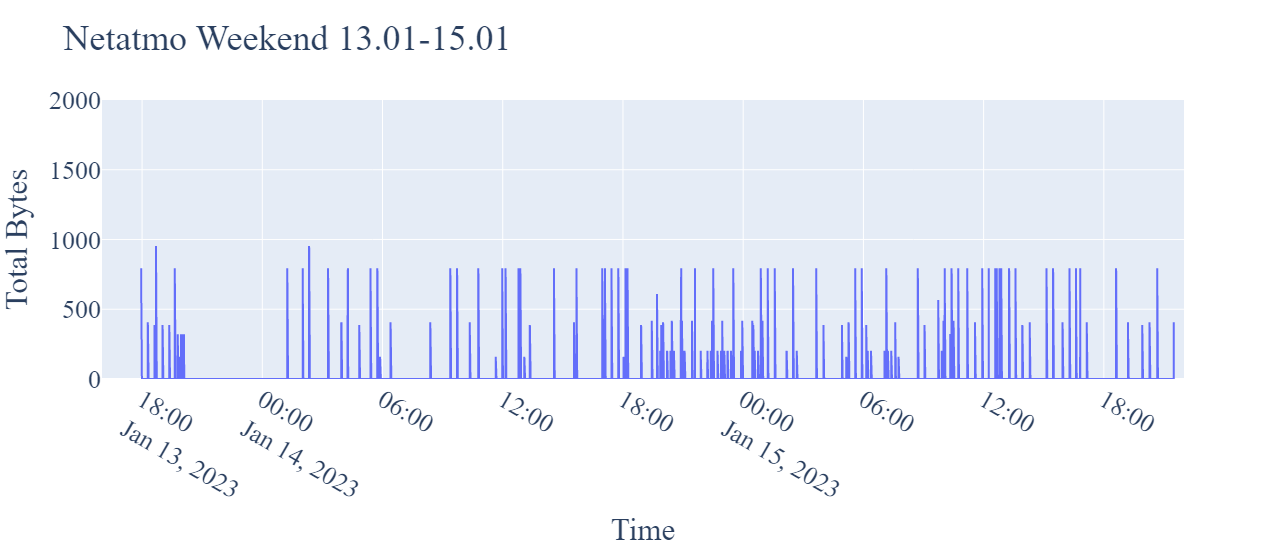
\includegraphics[width=1.1\hsize]{figures/Netatmo_Weekend_BigBytes_13.01-15.01.png}
    \end{subfigure}
    \begin{subfigure}[b]{0.47\textwidth}
        \includegraphics[width=1.1\hsize]{figures/Netatmo_Weekend_BigBytes_27.01-29.01.png}
    \end{subfigure}
    \begin{subfigure}[b]{0.47\textwidth}
        \includegraphics[width=1.1\hsize]{figures/Netatmo_Weekend_BigBytes_03.02-05.02.png}
    \end{subfigure}
    \begin{subfigure}[b]{0.47\textwidth}
        \includegraphics[width=1.1\hsize]{figures/Netatmo_Weekend_BigBytes_17.02-19.02.png}
    \end{subfigure}
    \begin{subfigure}[b]{0.47\textwidth}
        \includegraphics[width=1.1\hsize]{figures/Netatmo_Weekend_BigBytes_10.03-12.03.png}
    \end{subfigure}
    \begin{subfigure}[b]{0.47\textwidth}
        \includegraphics[width=1.1\hsize]{figures/Netatmo_Weekend_BigBytes_28.03-30.03.png}
    \end{subfigure}
    \begin{subfigure}[b]{0.47\textwidth}
        \includegraphics[width=1.1\hsize]{figures/Netatmo_Weekend_BigBytes_31.03-02.04.png}
    \end{subfigure}
    \caption{Netatmo: Home-Weekends with Only Packets over 154 Bytes}
    \label{fig:NetatmoBigPackets}
\end{figure}

The graphs in Figure \ref{fig:NetatmoBigPackets} shows that it is possible to see if a home is occupied by looking at the packet sizes that are sent. The last evaluation on Netatmo Weekend events are comparing the graphs for bytes in Figure \ref{fig:NetatmoWeekendBytes} against values from the application of the device. This is presented in Figure \ref{fig:NetatmoWeekendBytesAndApp1} and \ref{fig:NetatmoWeekendBytesandApp2}. The graphs extracted from the app, Netatmo Home Coach, and the sensor values are in \(CO_2\). The y-axis, which are in ppm are not equal for each of the graphs from the app, as this is not possible to change. The x-axis are in time. 
\\\\
The Figures in \ref{fig:NetatmoWeekendBytesandApp1} and \ref{fig:NetatmoWeekendBytesandApp2} shows the same pattern as for the bytes from the traffic captures on the left side of the figure. When the home is not occupied, the \(CO_2\) value are not affected which the corresponding traffic flow in the byte-graphs shows, and when the home is occupied, the \(CO_2\) levels varies a lot and the corresponding traffic flow also varies a lot. 

\begin{figure}[H]
    \begin{subfigure}[b]{0.47\textwidth}
    \centering
        \tcbincludegraphics[size=fbox,width=1.1\hsize,height=0.15\vsize,colframe=green]{figures/Netatmo_Weekend_Bytes_13.01-15.01.png}
    \end{subfigure}
    \begin{subfigure}[b]{0.47\textwidth}
    \centering
        \tcbincludegraphics[size=fbox,width=1.1\hsize,height=0.15\vsize,colframe=green]{figures/Netatmo_Weekend_App_13.01-15.01.png}
    \end{subfigure}
    \begin{subfigure}[b]{0.47\textwidth}
    \centering
        \tcbincludegraphics[size=fbox,width=1.1\hsize,height=0.15\vsize,colframe=orange]{figures/Netatmo_Weekend_Bytes_23.12-25.12.png}
    \end{subfigure}
    \begin{subfigure}[b]{0.47\textwidth}
    \centering
        \tcbincludegraphics[size=fbox,width=1.1\hsize,height=0.15\vsize,colframe=orange]{figures/Netatmo_Weekend_App_23.12-25.12.png}
    \end{subfigure}
    \begin{subfigure}[b]{0.47\textwidth}
        \tcbincludegraphics[size=fbox,width=1.1\hsize,height=0.15\vsize,colframe=green]{figures/Netatmo_Weekend_Bytes_27.01-29.01.png}
    \end{subfigure}
    \begin{subfigure}[b]{0.47\textwidth}
        \tcbincludegraphics[size=fbox,width=1.1\hsize,height=0.15\vsize,colframe=green]{figures/Netatmo_Weekend_App_27.01-29.01.png}
    \end{subfigure}
    \begin{subfigure}[b]{0.47\textwidth}
        \tcbincludegraphics[size=fbox,width=1.1\hsize,height=0.15\vsize,colframe=orange]{figures/Netatmo_Weekend_Bytes_30.12-01.01.png}
    \end{subfigure}
    \begin{subfigure}[b]{0.47\textwidth}
        \tcbincludegraphics[size=fbox,width=1.1\hsize,height=0.15\vsize,colframe=orange]{figures/Netatmo_Weekend_App_30.12-01.01.png}
    \end{subfigure}    
    \begin{subfigure}[b]{0.47\textwidth}
        \tcbincludegraphics[size=fbox,width=1.1\hsize,height=0.15\vsize,colframe=green]{figures/Netatmo_Weekend_Bytes_03.02-05.02.png}
    \end{subfigure}
    \begin{subfigure}[b]{0.47\textwidth}
        \tcbincludegraphics[size=fbox,width=1.1\hsize,height=0.15\vsize,colframe=green]{figures/Netatmo_Weekend_App_03.02-05.02.png}
    \end{subfigure}
    \begin{subfigure}[b]{0.47\textwidth}
        \tcbincludegraphics[size=fbox,width=1.1\hsize,height=0.15\vsize,colframe=orange]{figures/Netatmo_Weekend_Bytes_20.01-22.01.png}
    \end{subfigure}
    \begin{subfigure}[b]{0.47\textwidth}
        \tcbincludegraphics[size=fbox,width=1.1\hsize,height=0.15\vsize,colframe=orange]{figures/Netatmo_Weekend_App_20.01-22.01.png}
    \end{subfigure}    
    \begin{subfigure}[b]{0.47\textwidth}
        \tcbincludegraphics[size=fbox,width=1.1\hsize,height=0.15\vsize,colframe=green]{figures/Netatmo_Weekend_Bytes_17.02-19.02.png}
    \end{subfigure}
    \hspace{0.6cm}
    \begin{subfigure}[b]{0.47\textwidth}
        \tcbincludegraphics[size=fbox,width=1.1\hsize,height=0.15\vsize,colframe=green]{figures/Netatmo_Weekend_App_17.02-19.02.png}
    \end{subfigure}
    \caption{Netatmo: Weekends at Home(green) and Gone(orange) Presented in Bytes and Compared to Corresponding Dates in App 1}
    \label{fig:NetatmoWeekendBytesandApp1}
\end{figure} 
\begin{figure}[H]
    \begin{subfigure}[b]{0.47\textwidth}
        \tcbincludegraphics[size=fbox,width=1.1\hsize,height=0.15\vsize,colframe=orange]{figures/Netatmo_Weekend_Bytes_10.02-12.02.png}
    \end{subfigure}
    \begin{subfigure}[b]{0.47\textwidth}
        \tcbincludegraphics[size=fbox,width=1.1\hsize,height=0.15\vsize,colframe=orange]{figures/Netatmo_Weekend_App_10.02-12.02.png}
    \end{subfigure}
    \begin{subfigure}[b]{0.47\textwidth}
        \tcbincludegraphics[size=fbox,width=1.1\hsize,height=0.15\vsize,colframe=green]{figures/Netatmo_Weekend_Bytes_10.03-12.03.png}
    \end{subfigure}
    \begin{subfigure}[b]{0.47\textwidth}
        \tcbincludegraphics[size=fbox,width=1.1\hsize,height=0.15\vsize,colframe=green]{figures/Netatmo_Weekend_App_10.03-12.03.png}
    \end{subfigure}
    \begin{subfigure}[b]{0.47\textwidth}
        \tcbincludegraphics[size=fbox,width=1.1\hsize,height=0.15\vsize,colframe=orange]{figures/Netatmo_Weekend_Bytes_24.02-26.02.png}
    \end{subfigure}
    \begin{subfigure}[b]{0.47\textwidth}
        \tcbincludegraphics[size=fbox,width=1.1\hsize,height=0.15\vsize,colframe=orange]{figures/Netatmo_Weekend_App_24.02-26.02.png}
    \end{subfigure}
    \begin{subfigure}[b]{0.47\textwidth}
        \tcbincludegraphics[size=fbox,width=1.1\hsize,height=0.15\vsize,colframe=green]{figures/Netatmo_Weekend_Bytes_28.03-30.03.png}
    \end{subfigure}
    \begin{subfigure}[b]{0.47\textwidth}
        \tcbincludegraphics[size=fbox,width=1.1\hsize,height=0.15\vsize,colframe=green]{figures/Netatmo_Weekend_App_28.03-30.03.png}
    \end{subfigure}
    \begin{subfigure}[b]{0.47\textwidth}
        \tcbincludegraphics[size=fbox,width=1.1\hsize,height=0.15\vsize,colframe=orange]{figures/Netatmo_Weekend_Bytes_03.03-05.03.png}
    \end{subfigure}
    \begin{subfigure}[b]{0.47\textwidth}
        \tcbincludegraphics[size=fbox,width=1.1\hsize,height=0.15\vsize,colframe=orange]{figures/Netatmo_Weekend_App_03.03-05.03.png}
    \end{subfigure}
   \begin{subfigure}[b]{0.47\textwidth}
        \tcbincludegraphics[size=fbox,width=1.1\hsize,height=0.15\vsize,colframe=green]{figures/Netatmo_Weekend_Bytes_31.03-02.04.png}
    \end{subfigure}
    \begin{subfigure}[b]{0.47\textwidth}
        \tcbincludegraphics[size=fbox,width=1.1\hsize,height=0.15\vsize,colframe=green]{figures/Netatmo_Weekend_App_31.03-02.04.png}
    \end{subfigure}
    \begin{subfigure}[b]{0.47\textwidth}
        \tcbincludegraphics[size=fbox,width=1.1\hsize,height=0.15\vsize,colframe=orange]{figures/Netatmo_Weekend_Bytes_17.03-19.03.png}
    \end{subfigure}
    \hspace{0.6cm}
    \begin{subfigure}[b]{0.47\textwidth}
        \tcbincludegraphics[size=fbox,width=1.1\hsize,height=0.15\vsize,colframe=orange]{figures/Netatmo_Weekend_App_17.03-19.03.png}
    \end{subfigure}
    \caption{Netatmo: Weekends at Home(green) and Gone(orange) Presented in Bytes and Compared to Corresponding Dates in App 2}
    \label{fig:NetatmoWeekendBytesandApp2}
\end{figure}

\subsection{Mill Sense}
For weekend testing with the device, Mill Sense, Table \ref{tab:MillWeekendHome} and \ref{tab:MillWeekendGone} presents the calculations on the pcaps for respectively Home and Gone Weekends. Average and standard deviation values from the tables are combined and compared in Table \ref{tab:MillWeekends}. Graphs of traffic flow are presented in Figure \ref{fig:MillWeekendBytes} for bytes and in Figure \ref{fig:MillWeekendPackets} for packets. The graphs marked in green on the figures are Home Weekends and are placed on the left side of the figures, while the graphs marked in orange on the figures are Gone Weekends and placed on the right side of the figures. The graphs in the same figure all have the same maximum values for the y-axis so they are easily comparable.

\begin{table}[H]
    \centering
    \caption{Mill: Weekend Calculations for Home}
    \begin{tabular}{|l|l|l|l|l|}
        \hline
        \textbf{Date}    & \textbf{Total pkt} & \textbf{Total bytes} & \textbf{Biggest src} & \textbf{Biggest dst} \\ \hline
        13.01-15.01      & 285,543            & 33,269,620           & 456 bytes            & 1,593 bytes          \\ \hline
        27.01-29.01      & 240,434            & 29,179,764           & 456 bytes            & 1,593 bytes          \\ \hline
        03.02-05.02      & 223,095            & 28,543,539           & 456 bytes            & 1,593 bytes          \\ \hline
        17.02-19.02      & 237,964            & 25,637,948           & 456 bytes            & 1,583 bytes          \\ \hline
        10.03-12.03      & 295,395            & 31,161,679           & 456 bytes            & 1,593 bytes          \\ \hline
        28.03-30.03      & 342,001            & 39,951,155           & 456 bytes            & 421 bytes            \\ \hline
        31.03-02.04      & 275,456            & 30,155,191           & 456 bytes            & 421 bytes            \\ \hline
    \end{tabular}
    \label{tab:MillHomeWeekends}
\end{table}

\begin{table}[H]
    \centering
    \caption{Mill: Weekend Calculations for Gone}
    \begin{tabular}{|l|l|l|l|l|}
        \hline
        \textbf{Date}    & \textbf{Total pkt} & \textbf{Total bytes} & \textbf{Biggest src} & \textbf{Biggest dst} \\ \hline
        23.12-25.12      & 259,516            & 34,066,162           & 456 bytes            & 421 bytes            \\ \hline
        30.12-01.01      & 255,487            & 32,809,172           & 456 bytes            & 421 bytes            \\ \hline
        20.01-22.01      & 256,455            & 29,417,721           & 456 bytes            & 421 bytes            \\ \hline
        10.02-12.02      & 270,718            & 30,482,741           & 456 bytes            & 421 bytes            \\ \hline
        24.02-26.02      & 218,536            & 25,525,312           & 456 bytes            & 421 bytes            \\ \hline
        03.03-05.03      & 236,655            & 23,064,715           & 456 bytes            & 421 bytes            \\ \hline
        17.03-19.03      & 278,146            & 28,612,487           & 456 bytes            & 421 bytes            \\ \hline
    \end{tabular}
    \label{tab:MillGoneWeekends}
\end{table}

\begin{table}[H]
    \centering
    \caption{Mill: Comparing Weekend Values}
    \begin{tabular}{ll|l|l|l|l|}
        \cline{3-6}
        \textbf{}                                           & \textbf{} & \textbf{Packets} & \textbf{Bytes} & \textbf{Biggest src} & \textbf{Biggest dst} \\ \hline
        \multicolumn{1}{|l|}{\multirow{2}{*}{\textbf{Average}}} & Home      & 271,413          & 31,128,414      & 456 bytes            & 1,257 bytes          \\ \cline{2-7} 
        \multicolumn{1}{|l|}{}                              & Gone      & 253,645          & 29,139,759      & 456 bytes            & 421 bytes            \\ \hline
        \multicolumn{1}{|l|}{\multirow{2}{*}{\textbf{SD}}}  & Home      & 41,205           & 4,546,021      & 0 bytes              & 571 bytes            \\ \cline{2-7} 
        \multicolumn{1}{|l|}{}                              & Gone      & 20,224           & 3,870,041       & 0 bytes              & 0 bytes              \\ \hline
    \end{tabular}
    \label{tab:MillWeekends}
\end{table}

\begin{figure} [H]
    \begin{subfigure}[b]{0.47\textwidth}
    \centering
        \tcbincludegraphics[size=fbox,width=1.1\hsize,colframe=green]{figures/Mill_Weekend_Packets_13.01-15.01.png}    
    \end{subfigure}
    \begin{subfigure}[b]{0.47\textwidth}
    \centering
        \tcbincludegraphics[size=fbox,width=1.1\hsize,colframe=orange]{figures/Mill_Weekend_Packets_23.12-25.12.png}
    \end{subfigure}
    \begin{subfigure}[b]{0.47\textwidth}
        \tcbincludegraphics[size=fbox,width=1.1\hsize,colframe=green]{figures/Mill_Weekend_Packets_27.01-29.01.png}
    \end{subfigure}
    \begin{subfigure}[b]{0.47\textwidth}
        \tcbincludegraphics[size=fbox,width=1.1\hsize,colframe=orange]{figures/Mill_Weekend_Packets_30.12-01.01.png}
    \end{subfigure}
    \begin{subfigure}[b]{0.47\textwidth}
        \tcbincludegraphics[size=fbox,width=1.1\hsize,colframe=green]{figures/Mill_Weekend_Packets_03.02-05.02.png}
    \end{subfigure}    
    \begin{subfigure}[b]{0.47\textwidth}
        \tcbincludegraphics[size=fbox,width=1.1\hsize,colframe=orange]{figures/Mill_Weekend_Packets_20.01-22.01.png}
    \end{subfigure}
    \begin{subfigure}[b]{0.47\textwidth}
        \tcbincludegraphics[size=fbox,width=1.1\hsize,colframe=green]{figures/Mill_Weekend_Packets_17.02-19.02.png}
    \end{subfigure}    
    \begin{subfigure}[b]{0.47\textwidth}
        \tcbincludegraphics[size=fbox,width=1.1\hsize,colframe=orange]{figures/Mill_Weekend_Packets_10.02-12.02.png}
    \end{subfigure}
    \begin{subfigure}[b]{0.47\textwidth}
        \tcbincludegraphics[size=fbox,width=1.1\hsize,colframe=green]{figures/Mill_Weekend_Packets_10.03-12.03.png}
    \end{subfigure}    
    \begin{subfigure}[b]{0.47\textwidth}
        \tcbincludegraphics[size=fbox,width=1.1\hsize,colframe=orange]{figures/Mill_Weekend_Packets_24.02-26.02.png}
    \end{subfigure}
    \begin{subfigure}[b]{0.47\textwidth}
        \tcbincludegraphics[size=fbox,width=1.1\hsize,colframe=green]{figures/Mill_Weekend_Packets_28.03-30.03.png}
    \end{subfigure}
    \begin{subfigure}[b]{0.47\textwidth}
        \tcbincludegraphics[size=fbox,width=1.1\hsize,colframe=orange]{figures/Mill_Weekend_Packets_03.03-05.03.png}
    \end{subfigure}
    \begin{subfigure}[b]{0.47\textwidth}
        \tcbincludegraphics[size=fbox,width=1.1\hsize,colframe=green]{figures/Mill_Weekend_Packets_31.03-02.04.png}
    \end{subfigure}
    \hspace{0.6cm}
    \begin{subfigure}[b]{0.47\textwidth}
        \tcbincludegraphics[size=fbox,width=1.1\hsize,colframe=orange]{figures/Mill_Weekend_Packets_17.03-19.03.png}
    \end{subfigure}
    \caption{Mill: Weekends at Home(green) and Gone(orange) Presented in Packets}
    \label{fig:MillWeekendPackets}
\end{figure}

\begin{figure}[H]
    \begin{subfigure}[b]{0.47\textwidth}
    \centering
        \tcbincludegraphics[size=fbox,width=1.1\hsize,colframe=green]{figures/Mill_Weekend_Bytes_13.01-15.01.png}
    \end{subfigure}
    \begin{subfigure}[b]{0.47\textwidth}
    \centering
        \tcbincludegraphics[size=fbox,width=1.1\hsize,colframe=orange]{figures/Mill_Weekend_Bytes_23.12-25.12.png}
    \end{subfigure}
    \begin{subfigure}[b]{0.47\textwidth}
        \tcbincludegraphics[size=fbox,width=1.1\hsize,colframe=green]{figures/Mill_Weekend_Bytes_27.01-29.01.png}
    \end{subfigure}
    \begin{subfigure}[b]{0.47\textwidth}
        \tcbincludegraphics[size=fbox,width=1.1\hsize,colframe=orange]{figures/Mill_Weekend_Bytes_30.12-01.01.png}
    \end{subfigure}
    \begin{subfigure}[b]{0.47\textwidth}
        \tcbincludegraphics[size=fbox,width=1.1\hsize,colframe=green]{figures/Mill_Weekend_Bytes_03.02-05.02.png}
    \end{subfigure}
    \begin{subfigure}[b]{0.47\textwidth}
        \tcbincludegraphics[size=fbox,width=1.1\hsize,colframe=orange]{figures/Mill_Weekend_Bytes_20.01-22.01.png}
    \end{subfigure}
    \begin{subfigure}[b]{0.47\textwidth}
        \tcbincludegraphics[size=fbox,width=1.1\hsize,colframe=green]{figures/Mill_Weekend_Bytes_17.02-19.02.png}
    \end{subfigure}
    \begin{subfigure}[b]{0.47\textwidth}
        \tcbincludegraphics[size=fbox,width=1.1\hsize,colframe=orange]{figures/Mill_Weekend_Bytes_10.02-12.02.png}
    \end{subfigure}
    \begin{subfigure}[b]{0.47\textwidth}
        \tcbincludegraphics[size=fbox,width=1.1\hsize,colframe=green]{figures/Mill_Weekend_Bytes_10.03-12.03.png}
    \end{subfigure}
    \begin{subfigure}[b]{0.47\textwidth}
        \tcbincludegraphics[size=fbox,width=1.1\hsize,colframe=orange]{figures/Mill_Weekend_Bytes_24.02-26.02.png}
    \end{subfigure}
    \begin{subfigure}[b]{0.47\textwidth}
        \tcbincludegraphics[size=fbox,width=1.1\hsize,colframe=green]{figures/Mill_Weekend_Bytes_28.03-30.03.png}
    \end{subfigure}
    \begin{subfigure}[b]{0.47\textwidth}
        \tcbincludegraphics[size=fbox,width=1.1\hsize,colframe=orange]{figures/Mill_Weekend_Bytes_03.03-05.03.png}
    \end{subfigure}
   \begin{subfigure}[b]{0.47\textwidth}
        \tcbincludegraphics[size=fbox,width=1.1\hsize,colframe=green]{figures/Mill_Weekend_Bytes_31.03-02.04.png}
    \end{subfigure}
    \hspace{0.6cm}
    \begin{subfigure}[b]{0.47\textwidth}
        \tcbincludegraphics[size=fbox,width=1.1\hsize,colframe=orange]{figures/Mill_Weekend_Bytes_17.03-19.03.png}
    \end{subfigure}
    \caption{Mill: Weekends at Home(green) and Gone(orange) Presented in Bytes}
    \label{fig:MillWeekendBytes}
\end{figure}

Looking at the values in Table \ref{tab:MillHomeWeekends} and \ref{tab:MillGoneWeekends}, the total packets and bytes in the pcaps stay the same whether or not it's a Home or Gone Weekend. In regards of the largest packets, all the Gone-Weekends have the same size; 456 bytes for packets sent from the device and 421 bytes for packets sent to the device. For the first 5 Home-Weekends it looks like there's a pattern change that the device receives much bigger packets than in a Gone-Weekend with a size 1,583 an 1,593 bytes, but as the last two Home-Weekend shows their biggest packet is actually the same as for a Gone-Weekend. The graphs in Figure \ref{fig:MillWeekendPackets} and \ref{fig:MillWeekendBytes} the traffic pattern for Home and Gone Weekends look the same. There are variations in the same category, but not a constant same variation for Home or Gone. 

\newpage
\subsection{Nedis}
For Weekend testing on the device Nedis, both tables for calculations and figures for graphs are presented to analyze the traffic patterns during the tests. In Table \ref{tab:NedisHomeWeekends} and \ref{tab:NedisGoneWeekends} the calculations for the Home and Gone Weekends are presented. The values included are total amount of packets, total bytes sent and received from the device, the biggest packet sent in bytes and the biggest packet received in bytes. Table \ref{tab:NedisWeekends} compares the average and standard deviation values for respectively all the weekends home and all the weekends gone. Figure \ref{fig:NedisWeekendPackets} presents the graphs for weekend traffic in regards of packets and Figure \ref{fig:NedisWeekendBytes} presents the graphs for weekend traffic in regards of bytes. Both figures have the Home-Weekends placed on the left side of the figure framed in green and the Gone-Weekends placed on the right side of the figure framed in orange.  

\begin{table}[H]
    \caption{Nedis: Weekend Calculations for Home}
    \begin{tabular}{|l|l|l|l|l|l|}
        \hline
        \textbf{Date}    & \textbf{Total pkt} & \textbf{Total bytes} & \textbf{Biggest src} & \textbf{Biggest dst} \\ \hline
        13.01-15.01      & 565,380            & 66,062,682           & 485 bytes            & 522 bytes            \\ \hline
        27.01-29.01      & 546,269            & 58,677,501           & 424 bytes            & 522 bytes            \\ \hline
        03.02-05.02      & 501,936            & 62,219,835           & 485 bytes            &    522 bytes            \\ \hline
        17.02-19.02      & 501,747            & 64,037,197           & 485 bytes            & 522 bytes            \\ \hline
        10.03-12.03      & 482,205            & 60,333,999           & 485 bytes            & 522 bytes            \\ \hline
        28.03-30.03      & 578,033            & 65,159,251           & 424 bytes            & 426 bytes            \\ \hline
        31.03-02.04      & 621,200            & 81,810,849           & 485 bytes            & 458 bytes            \\ \hline
    \end{tabular}
    \label{tab:NedisHomeWeekends}
\end{table}

\begin{table}[H]
    \caption{Nedis: Weekend Calculations for Gone}
    \begin{tabular}{|l|l|l|l|l|l|}
        \hline
        \textbf{Date} & \textbf{Total pkt} & \textbf{Total bytes} & \textbf{Biggest src} & \textbf{Biggest dst} \\ \hline
        13.01-15.01   & 678,979            & 98,642,277           & 485 bytes            & 522 bytes            \\ \hline
        27.01-29.01   & 655,417            & 91,850,956           & 485 bytes            & 650 bytes            \\ \hline
        03.02-05.02   & 518,316            & 66,069,105           & 485 bytes            & 522 bytes            \\ \hline
        17.02-19.02   & 426,157            & 53,137,691           & 424 bytes            & 522 bytes            \\ \hline
        10.03-12.03   & 357,715            & 42,390,770           & 424 bytes            & 522 bytes            \\ \hline
        28.03-30.03   & 507,506            & 65,163,914           & 485 bytes            & 522 bytes            \\ \hline
        31.03-02.04   & 634,018            & 87,175,396           & 554 bytes            & 522 bytes            \\ \hline
    \end{tabular}
    \label{tab:NedisGoneWeekends}
\end{table}

\begin{table}[H]
    \centering
    \caption{Nedis: Comparing Weekend Values}
    \begin{tabular}{ll|l|l|l|l|}
        \cline{3-6}
        \textbf{}                                           & \textbf{} & \textbf{Packets} & \textbf{Bytes} & \textbf{Biggest src} & \textbf{Biggest dst} \\ \hline
        \multicolumn{1}{|l|}{\multirow{2}{*}{\textbf{AVG}}} & Home      & 542,396          & 65,471,616     & 470 bytes            & 522 bytes            \\ \cline{2-6} 
        \multicolumn{1}{|l|}{}                              & Gone      & 539,730          & 72,061,444     & 477 bytes            & 540 bytes            \\ \hline
        \multicolumn{1}{|l|}{\multirow{2}{*}{\textbf{SD}}}  & Home      & 49,893           & 7,665,988      & 30 bytes             & 40 bytes             \\ \cline{2-6} 
        \multicolumn{1}{|l|}{}                              & Gone      & 121,922          & 21,010,071     & 44 bytes             & 48 bytes             \\ \hline
    \end{tabular}
    \label{tab:NedisWeekends}
\end{table}

\begin{figure} [H]
    \begin{subfigure}[b]{0.47\textwidth}
    \centering
        \tcbincludegraphics[size=fbox,width=1.1\hsize,colframe=green]{figures/Nedis_Weekend_Packets_13.01-15.01.png}    
    \end{subfigure}
    \begin{subfigure}[b]{0.47\textwidth}
    \centering
        \tcbincludegraphics[size=fbox,width=1.1\hsize,colframe=orange]{figures/Nedis_Weekend_Packets_23.12-25.12.png}
    \end{subfigure}
    \begin{subfigure}[b]{0.47\textwidth}
        \tcbincludegraphics[size=fbox,width=1.1\hsize,colframe=green]{figures/Nedis_Weekend_Packets_27.01-29.01.png}
    \end{subfigure}
    \begin{subfigure}[b]{0.47\textwidth}
        \tcbincludegraphics[size=fbox,width=1.1\hsize,colframe=orange]{figures/Nedis_Weekend_Packets_30.12-01.01.png}
    \end{subfigure}
    \begin{subfigure}[b]{0.47\textwidth}
        \tcbincludegraphics[size=fbox,width=1.1\hsize,colframe=green]{figures/Nedis_Weekend_Packets_03.02-05.02.png}
    \end{subfigure}    
    \begin{subfigure}[b]{0.47\textwidth}
        \tcbincludegraphics[size=fbox,width=1.1\hsize,colframe=orange]{figures/Nedis_Weekend_Packets_20.01-22.01.png}
    \end{subfigure}
    \begin{subfigure}[b]{0.47\textwidth}
        \tcbincludegraphics[size=fbox,width=1.1\hsize,colframe=green]{figures/Nedis_Weekend_Packets_17.02-19.02.png}
    \end{subfigure}    
    \begin{subfigure}[b]{0.47\textwidth}
        \tcbincludegraphics[size=fbox,width=1.1\hsize,colframe=orange]{figures/Nedis_Weekend_Packets_10.02-12.02.png}
    \end{subfigure}
    \begin{subfigure}[b]{0.47\textwidth}
        \tcbincludegraphics[size=fbox,width=1.1\hsize,colframe=green]{figures/Nedis_Weekend_Packets_10.03-12.03.png}
    \end{subfigure}    
    \begin{subfigure}[b]{0.47\textwidth}
        \tcbincludegraphics[size=fbox,width=1.1\hsize,colframe=orange]{figures/Nedis_Weekend_Packets_24.02-26.02.png}
    \end{subfigure}
    \begin{subfigure}[b]{0.47\textwidth}
        \tcbincludegraphics[size=fbox,width=1.1\hsize,colframe=green]{figures/Nedis_Weekend_Packets_28.03-30.03.png}
    \end{subfigure}
    \begin{subfigure}[b]{0.47\textwidth}
        \tcbincludegraphics[size=fbox,width=1.1\hsize,colframe=orange]{figures/Nedis_Weekend_Packets_03.03-05.03.png}
    \end{subfigure}
    \begin{subfigure}[b]{0.47\textwidth}
        \tcbincludegraphics[size=fbox,width=1.1\hsize,colframe=green]{figures/Nedis_Weekend_Packets_31.03-02.04.png}
    \end{subfigure}
    \hspace{0.6cm}
    \begin{subfigure}[b]{0.47\textwidth}
        \tcbincludegraphics[size=fbox,width=1.1\hsize,colframe=orange]{figures/Nedis_Weekend_Packets_17.03-19.03.png}
    \end{subfigure}
    \caption{Nedis: Weekends at Home(green) and Gone(orange) Presented in Packets}
    \label{fig:NedisWeekendPackets}
\end{figure}

\begin{figure}[H]
    \begin{subfigure}[b]{0.47\textwidth}
    \centering
        \tcbincludegraphics[size=fbox,width=1.1\hsize,colframe=green]{figures/Nedis_Weekend_Bytes_13.01-15.01.png}
    \end{subfigure}
    \begin{subfigure}[b]{0.47\textwidth}
    \centering
        \tcbincludegraphics[size=fbox,width=1.1\hsize,colframe=orange]{figures/Nedis_Weekend_Bytes_23.12-25.12.png}
    \end{subfigure}
    \begin{subfigure}[b]{0.47\textwidth}
        \tcbincludegraphics[size=fbox,width=1.1\hsize,colframe=green]{figures/Nedis_Weekend_Bytes_27.01-29.01.png}
    \end{subfigure}
    \begin{subfigure}[b]{0.47\textwidth}
        \tcbincludegraphics[size=fbox,width=1.1\hsize,colframe=orange]{figures/Nedis_Weekend_Bytes_30.12-01.01.png}
    \end{subfigure}
    \begin{subfigure}[b]{0.47\textwidth}
        \tcbincludegraphics[size=fbox,width=1.1\hsize,colframe=green]{figures/Nedis_Weekend_Bytes_03.02-05.02.png}
    \end{subfigure}
    \begin{subfigure}[b]{0.47\textwidth}
        \tcbincludegraphics[size=fbox,width=1.1\hsize,colframe=orange]{figures/Nedis_Weekend_Bytes_20.01-22.01.png}
    \end{subfigure}
    \begin{subfigure}[b]{0.47\textwidth}
        \tcbincludegraphics[size=fbox,width=1.1\hsize,colframe=green]{figures/Nedis_Weekend_Bytes_17.02-19.02.png}
    \end{subfigure}
    \begin{subfigure}[b]{0.47\textwidth}
        \tcbincludegraphics[size=fbox,width=1.1\hsize,colframe=orange]{figures/Nedis_Weekend_Bytes_10.02-12.02.png}
    \end{subfigure}
    \begin{subfigure}[b]{0.47\textwidth}
        \tcbincludegraphics[size=fbox,width=1.1\hsize,colframe=green]{figures/Nedis_Weekend_Bytes_10.03-12.03.png}
    \end{subfigure}
    \begin{subfigure}[b]{0.47\textwidth}
        \tcbincludegraphics[size=fbox,width=1.1\hsize,colframe=orange]{figures/Nedis_Weekend_Bytes_24.02-26.02.png}
    \end{subfigure}
    \begin{subfigure}[b]{0.47\textwidth}
        \tcbincludegraphics[size=fbox,width=1.1\hsize,colframe=green]{figures/Nedis_Weekend_Bytes_28.03-30.03.png}
    \end{subfigure}
    \begin{subfigure}[b]{0.47\textwidth}
        \tcbincludegraphics[size=fbox,width=1.1\hsize,colframe=orange]{figures/Nedis_Weekend_Bytes_03.03-05.03.png}
    \end{subfigure}
   \begin{subfigure}[b]{0.47\textwidth}
        \tcbincludegraphics[size=fbox,width=1.1\hsize,colframe=green]{figures/Nedis_Weekend_Bytes_31.03-02.04.png}
    \end{subfigure}
    \hspace{0.6cm}
    \begin{subfigure}[b]{0.47\textwidth}
        \tcbincludegraphics[size=fbox,width=1.1\hsize,colframe=orange]{figures/Nedis_Weekend_Bytes_17.03-19.03.png}
    \end{subfigure}
    \caption{Nedis: Weekends at Home(green) and Gone(orange) Presented in Bytes}
    \label{fig:NedisWeekendBytes}
\end{figure}

The results in Table \ref{tab:NedisHomeWeekends} and \ref{tab:NedisGoneWeekends} shows that the amount of packets does not change whether the home is occupied or not. Both tables shows that there are sent and received around 500,000 to 600,000 packets regardless if the user is home or not. The amount of bytes received and sent varies a lot in both the tables from 58,677,501 bytes to 81,810,849 bytes for the Home-Weekends and from 42,390,770 bytes to 98,642,277 bytes for the Gone-Weekends. Also looking at the biggest packets received and sent are very similar in both Home and Gone Weekends. Table \ref{tab:NedisWeekends} also shows the same results as discussed earlier. Neither average values for packets, bytes or biggest packets received or sent differs significantly from one another. The standard deviation for Gone-Weekends are some higher than Home-Weekends which means that the values differ more from each other, but since the average is similar and the values differ both higher and lower than the average, it is still not possible to see any differences here.  